%-------------------------------------------------------%
%       Snakemake-Intro for HPC Users                   %
%-------------------------------------------------------%


% this code will compile the document as handout with
% $ pdflatex -synctex=1 -interaction=nonstopmode "\def\ishandout{1} \input{Snakemake_HPC_Users.tex}"
\ifdefined\ishandout
\PassOptionsToClass{handout}{beamer}
\fi

\documentclass[english,xcolor=pdftex,dvipsnames,aspectratio=<+++ if course.aspectratio is defined +++><++course.aspectratio++><+++else+++>43<+++endif+++>]{beamer} 

% to typeset only a few slide sets, set them here during development
%\includeonly{Why_Workflows}

\usepackage{etoolbox}
%\setbeamertemplate{mini frames}[box]
\usepackage{babel}
\usepackage[utf8]{inputenc}
\usepackage[T1]{fontenc}
\usepackage{amsfonts,amsmath,amssymb}
\usepackage{textgreek}
\usepackage{wrapfig}

\usepackage[load-configurations=binary,binary-units=true]{siunitx}
\usepackage[normalem]{ulem} % for strikethrough with \sout

\usepackage{color,colortbl}
\usepackage{upquote}

\usepackage{pifont}

\definecolor{pblue}{RGB}{45,106,148}
\definecolor{pdarkblue}{RGB}{35,71,100}
\definecolor{plightblue}{RGB}{90,159,212}
\definecolor{pyellow}{RGB}{255,212,59}
\definecolor{pdarkyellow}{RGB}{255,188,41}
\definecolor{orange}{RGB}{255,165,0}
\definecolor{plightyellow}{RGB}{255,232,115}
\definecolor{pdarkgrey}{RGB}{100,100,100}
\definecolor{pgrey}{RGB}{153,153,153}
\definecolor{plightgrey}{RGB}{233,233,233}
\definecolor{plightgrey2}{RGB}{247,247,247}
\definecolor{pnavy}{RGB}{0,0,170}
\definecolor{BrickRed}{RGB}{150,22,11}
\definecolor{BlueViolet}{RGB}{138, 43, 226}
\definecolor{PineGreen}{RGB}{0, 51, 0}
\definecolor{light-gray}{gray}{0.95}

\definecolor{UniRot}{RGB}{193,0,42}
\definecolor{UniDunkelGrau}{RGB}{99,99,99}
\definecolor{UniHellGrau}{RGB}{172,172,172}

\definecolor{UrlColor}{rgb}{0,0.08,0.45}
\definecolor{links}{rgb}{0,0,0}

\usetheme{<++layout.theme++>} % Pittsburgh, CambridgeUS
\usecolortheme{<++layout.colortheme++>} %wolverine | crane | beaver | seahorse
\useinnertheme{rounded} 
\useoutertheme{default}
\usefonttheme{default}
%\setbeamercovered{transparent}
\setbeamertemplate{footline}[frame number]

% remove the navigation symbols
\setbeamertemplate{navigation symbols}{}

% side margins
\setbeamersize{text margin left=0.5cm, text margin right=0.5cm}

\setbeamercolor{structure}{<++layout.beamercolor_structure++>}% to modify  immediately all palettes
\setbeamercolor{title}{<++layout.beamercolor_title++>}
\setbeamercolor{title in head/foot}{<++layout.beamercolor_title_head++>}

\setbeamercolor{block title}{<++layout.beamercolor_block_title++>}
\setbeamercolor{block body}{<++layout.beamercolor_block_body++>}

% \setbeamercolor{block title}{fg=white,bg=orange}
\setbeamercolor{block title alerted}{<++layout.beamercolor_block_title++>}
\setbeamercolor{block title example}{<++layout.beamercolor_block_title++>}

% saved commas in options
\newcommand{\safeopt}[1]{{{#1}}}

% enables two line cols in tabular envs
\newcommand{\specialcell}[2][c]{%
  \begin{tabular}[#1]{@{}c@{}}#2\end{tabular}}
\usepackage{subfig}
\usepackage{tikz}
\usetikzlibrary{arrows,shapes,snakes,backgrounds,positioning,shadows,decorations,trees,decorations.pathreplacing, graphs}
\usepackage{tkz-graph}

%\usepackage{tikzpeople}
\usepackage{smartdiagram}
\usesmartdiagramlibrary{additions}

%\usepackage{mdframed}

\usepackage{adjustbox} % to adjust tikzpictures within slides


\addtobeamertemplate{footline}{}{%
\begin{tikzpicture}[remember picture,overlay]
\node[anchor=south west,yshift=2pt] at (current page.south west) {\includegraphics[height=0.8cm]{../images/logos/zdv_logo.png}};
\end{tikzpicture}}

\usepackage[tikz]{bclogo}
\newenvironment{task}[1][Task]{\bclogo[arrondi=0.1,logo=\bcoutil]{#1}}{\endbclogo}
\newenvironment{docs}[1][Documentation]{\bclogo[arrondi=0.1,logo=\bcplume]{#1}}{\endbclogo}
\newenvironment{hint}[1][Hint]{\bclogo[arrondi=0.1,logo=\bcinfo]{#1}}{\endbclogo}
\newenvironment{warning}[1][Warning]{\bclogo[arrondi=0.1,logo=\bcattention]{#1}}{\endbclogo}
% ``d/Definition'' is already defined ;-)
\newenvironment{explanation}[1][Definition]{\bclogo[arrondi=0.1,logo=\bcplume]{#1}}{\endbclogo}
\newenvironment{question}[1][Question]{\bclogo[arrondi=0.1,logo=\bcquestion]{#1}}{\endbclogo}


%%%%%%%%%%%%%%%%%
%% PLEASE NOTE %%
%%%%%%%%%%%%%%%%%
% frames containing ``Hand Out'' or ``Interlude'' should be started:

% \setcounter{preframe_handson}{\value{handson}}
% \begin{frame}[fragile]
%   \setcounter{handson}{\value{preframe_handson}}
%   \frametitle{\HandsOn{Using \texttt{find}}}

% or

% \setcounter{preframe_interlude}{\value{interlude}}
% \begin{frame}[fragile]
%   \setcounter{interlude}{\value{preframe_interlude}}
%   \frametitle{Interlude -- Parameter Extension}

% respectively.

\newcounter{handson}
\setcounter{handson}{1}
\newcounter{preframe_handson}
\setcounter{preframe_handson}{1}
\newcommand{\HandsOn}[1]{Hands On \Roman{handson} -- #1 \addtocounter{handson}{1}}
%\newcommand{\HandsOn}[1]{Hands On -- #1}

%TODO: Merge ``HandsOn'' && ``Excercise''
\newcounter{exercise}
\setcounter{exercise}{1}
% \newcommand{\Exercise}{\theexercise . Excercise \addtocounter{exercise}{1}}

% Bugfix of the Exercise command: avoid the annoying counter
\newcommand{\Exercise}{\theexercise . Excercise \addtocounter{exercise}{1}}

\newcounter{interlude}
\setcounter{interlude}{1}
\newcounter{preframe_interlude}
\setcounter{preframe_interlude}{1}

%\newcommand{\Interlude}[1]{Interlude \Roman{interlude} -- #1 \addtocounter{interlude}{1}}

% Bugfix of the Interlude command: avoid the annoying counter!
\newcommand{\Interlude}[1]{Interlude -- #1}

\usepackage{marvosym}
\usepackage{multicol}

\usepackage{hhline}

\usepackage{times}

% will decrease the font size for one frame
\newcommand\Fontvi{\fontsize{6}{7.2}\selectfont}
% 
\usepackage{dirtree,float} % for directory tree listings
\usepackage[nodisplayskipstretch]{setspace}


\usepackage{verbatim}
\usepackage{listings}

\newcommand\YAMLcolonstyle{\color{red}\mdseries}
\newcommand\YAMLkeystyle{\color{black}\bfseries}
\newcommand\YAMLvaluestyle{\color{blue}\mdseries}

\makeatletter

% here is a macro expanding to the name of the language
% (handy if you decide to change it further down the road)
\newcommand\language@yaml{yaml}

\expandafter\expandafter\expandafter\lstdefinelanguage
\expandafter{\language@yaml}
{
	keywords={true,false,null,y,n},
	keywordstyle=\color{darkgray}\bfseries,
	basicstyle=\YAMLkeystyle,                                 % assuming a key comes first
	sensitive=false,
	comment=[l]{\#},
	morecomment=[s]{/*}{*/},
	commentstyle=\color{purple}\ttfamily,
	stringstyle=\YAMLvaluestyle\ttfamily,
	moredelim=[l][\color{orange}]{\&},
	moredelim=[l][\color{magenta}]{*},
	moredelim=**[il][\YAMLcolonstyle{:}\YAMLvaluestyle]{:},   % switch to value style at :
	morestring=[b]',
	morestring=[b]",
	literate =    {---}{{\ProcessThreeDashes}}3
	{>}{{\textcolor{red}\textgreater}}1     
	{|}{{\textcolor{red}\textbar}}1 
	{\ -\ }{{\mdseries\ -\ }}3,
}

% switch to key style at EOL
\lst@AddToHook{EveryLine}{\ifx\lst@language\language@yaml\YAMLkeystyle\fi}
\makeatother

\newcommand\ProcessThreeDashes{\llap{\color{cyan}\mdseries-{-}-}}


\makeatletter
\newcommand\applyCurrentFontsize
{%
	% we first save the current fontsize, baseline-skip,
	% and listings' basicstyle
	\let\f@sizeS@ved\f@size%
	\let\f@baselineskipS@ved\f@baselineskip%
	\let\basicstyleS@ved\lst@basicstyle%
	% we now change the fontsize of listings' basicstyle
	\renewcommand\lst@basicstyle%
	{%
		\basicstyleS@ved%
		\fontsize{\f@sizeS@ved}{\f@baselineskipS@ved}%
		\selectfont%
	}%
}
\makeatother

\newcommand{\altverb}[2][{}]{\colorbox{plightgrey}{\applyCurrentFontsize \lstinline[language={#1}]{#2}}}



\lstloadlanguages{Python,bash,C++}
\lstset{showspaces=false,
basicstyle=\small,
showstringspaces=false}

\lstdefinestyle{tree}{
    literate=
    {├}{{smash{raisebox{-1ex}{rule{1pt}{baselineskip}}}raisebox{0.5ex}{rule{1ex}{1pt}}}}1 
    {─}{{raisebox{0.5ex}{rule{1.5ex}{1pt}}}}1 
    {└}{{smash{raisebox{0.5ex}{rule{1pt}{dimexprbaselineskip-1.5ex}}}raisebox{0.5ex}{rule{1ex}{1pt}}}}1 
  }

%default python listings:
\lstdefinestyle{Python}
{
  language=Python,
  basicstyle=\small,
  showstringspaces=false,
  stepnumber=5,
  numberstyle=\tiny,
  numbersep=5pt,
  showspaces=false,
  frame=single,
  framerule=0.4pt,
  rulecolor=\color{pgrey},
  backgroundcolor=\color{white},
  stringstyle=\color{BrickRed},
  keywordstyle=\color{BlueViolet}\bfseries,
  commentstyle=\color{PineGreen}\bfseries,
  identifierstyle={},
  emph={[10]self}, emphstyle={[10]\color{pblue}},
  emph={[11]yield}, emphstyle={[11]\color{pblue}},
  moredelim=**[is][\bfseries\color{red}]{@}{@},
  literate={\\@}{{\makeatletter @ \makeatother}}1
}

\lstdefinestyle{R}
{
  language=R,
  basicstyle=\small,
  showstringspaces=false,
  stepnumber=5,
  numberstyle=\tiny,
  numbersep=5pt,
  showspaces=false,
  frame=single,
  framerule=0.4pt,
  rulecolor=\color{pgrey},
  backgroundcolor=\color{white},
  stringstyle=\color{BrickRed},
  keywordstyle=\color{BlueViolet}\bfseries,
  commentstyle=\color{PineGreen}\bfseries,
  identifierstyle={},
  emph={[10]self}, emphstyle={[10]\color{pblue}},
  emph={[11]yield}, emphstyle={[11]\color{pblue}},
}

%default python listings:
\lstdefinestyle{C++}
{
  language=C++,
  basicstyle=\small,
  showstringspaces=false,
  stepnumber=5,
  numberstyle=\tiny,
  numbersep=5pt,
  showspaces=false,
  frame=single,
  framerule=0.4pt,
  rulecolor=\color{pgrey},
  backgroundcolor=\color{white},
  stringstyle=\color{BrickRed},
  keywordstyle=\color{BlueViolet}\bfseries,
  commentstyle=\color{PineGreen}\bfseries,
  identifierstyle={},
  emph={[10]self}, emphstyle={[10]\color{pblue}},
  emph={[11]yield}, emphstyle={[11]\color{pblue}},
}

\newcommand{\CC}{C\nolinebreak\hspace{-.05em}\raisebox{1ex}{\tiny\bf +}\nolinebreak\hspace{-.10em}\raisebox{1ex}{\tiny\bf +}}

%default shell listings:
\lstdefinestyle{Shell}
{
  language=Bash,
  basicstyle=\ttfamily\small,
  showstringspaces=false,
  frame=single,
  framerule=0.4pt,
  rulecolor=\color{pgrey},
  backgroundcolor=\color{plightgrey2},
  stringstyle=\color{BrickRed},
  keywordstyle=\color{BlueViolet},
  commentstyle=\color{PineGreen}\bfseries,
  identifierstyle=\color{black},
  emph={[10]\$,>>>}, emphstyle={[10]\color{pblue}},
  moredelim=**[is][\bfseries\color{red}]{@}{@},
  literate={\\@}{{\makeatletter @ \makeatother}}1
}

%default plain listings (e.g. for config files):https://www.google.com/search?client=firefox-b-e&q=conrad
\lstdefinestyle{Plain}
{ 
  stepnumber=5,
  numberstyle=\tiny,
  numbersep=5pt,
  language=Bash,
  basicstyle=\ttfamily\small,
  showstringspaces=false,
  frame=single,
  framerule=0.4pt,
  rulecolor=\color{pgrey},
  backgroundcolor=\color{plightgrey2},
  stringstyle=\color{black},
  keywordstyle=\color{black},
  commentstyle=\color{blue}\bfseries,
  identifierstyle=\color{black},
  breaklines=true,
  emph={[10]\$,>>>}, emphstyle={[10]\color{pblue}}
}

\lstdefinelanguage{XML}
{
  frame=single,
  framerule=0.4pt,
  rulecolor=\color{pgrey},
  backgroundcolor=\color{plightgrey2},
  stringstyle=\color{black},
  keywordstyle=\color{black},
  commentstyle=\color{blue}\bfseries,
  identifierstyle=\color{black},
  emph={[10]\$,>>>}, emphstyle={[10]\color{pblue}}
  morestring=[b]",
  morestring=[s]{>}{<},
  morecomment=[s]{<?}{?>},
  morekeywords={xmlns,version,type}% list your attributes here
}

\newcommand{\bibtex}{\textsc{Bib}\TeX}

%%% https://tex.stackexchange.com/questions/99316/symbol-for-external-links
\newcommand{\LinkSymbol}{%
  \tikz[x=1.2ex, y=1.2ex, baseline=-0.05ex]{% 
    \begin{scope}[x=1ex, y=1ex]
      \clip (-0.1,-0.1) 
      --++ (-0, 1.2) 
      --++ (0.6, 0) 
      --++ (0, -0.6) 
      --++ (0.6, 0) 
      --++ (0, -1);
      \path[draw, 
      line width = 0.5, 
      rounded corners=0.5] 
      (0,0) rectangle (1,1);
    \end{scope}
    \path[draw, line width = 0.5] (0.5, 0.5) 
    -- (1, 1);
    \path[draw, line width = 0.5] (0.6, 1) 
    -- (1, 1) -- (1, 0.6);
  }
}
\newcommand{\lhref}[2]{\href{#1}{#2\,\LinkSymbol}}

%%%% shortcuts for uniform appearance of common strings %%%%
\newcommand{\slurm}{\textsc{slurm}~}
\makeatletter
\newcommand{\rmnum}[1]{\romannumeral #1}
\newcommand{\Rmnum}[1]{\expandafter\@slowromancap\romannumeral #1@}
\makeatother

%%%% nicer typesetting the snakemake project
\newcommand{\Snakemake}{\mbox{
	\begingroup\normalfont
	\includegraphics[height=\texorpdfstring{\fontcharht\font`\B}{1.2ex}]{logos/Snakemake.png}
	\textbf{Snakemake}
    \endgroup}
}


%\newcommand{\pathtoexercise}[1]{\path{/lustre/project/m2_jgu-ngstraing/workflows/#1}}
%\newcommand{\pathtoexercise}[1]{\path{ \DTLfetch{data}{thekey}{#1}{thevalue}   }}
\newcommand{\pathtoclozure}[1]{\path{workflows/tutorial/#1}}
\newcommand{\pathtosolutions}[1]{\path{/lustre/project/hpckurs/solutions/#1}}

\setcounter{tocdepth}{1}

% this allows turning of footlines for particular slides
\setbeamertemplate{footline}[frame number]
% to use it, perform:

% \begin{frame}
% normal frame
% \end{frame}
% 
% \begingroup
% \setbeamertemplate{footline}{}
% \begin{frame}
% without footline
% \end{frame}
% \endgroup

%--------------------%
% Meta-Info 
%--------------------%


\author[Snakemake Teaching Alliance]{The "Snakemake Teaching Alliance"}
\date{<++course.date++>}

\hypersetup{colorlinks,linkcolor=,urlcolor=links}

\graphicspath{{../images/}{../logos}}


% Passe captions an
\setbeamertemplate{caption}{\insertcaption}
% \setbeamerfont{caption}{size=\scriptsize}
\setlength\abovecaptionskip{-2.5pt}
\setlength\belowcaptionskip{0pt}



% For every picture that defines or uses external nodes, you'll have to
% apply the 'remember picture' style. To avoid some typing, we'll apply
% the style to all pictures.
\tikzstyle{every picture}+=[remember picture]
\tikzstyle{na} = [baseline=-.5ex]

% Add an include hook to error when a file is missing,
% to be able to recognize missing \include files on the
% CI.
% from: https://tex.stackexchange.com/questions/620515/how-to-force-latex-to-error-when-an-include-file-is-missing-misspelled
\makeatletter
\def\mkfilename#1{%
  \if\relax\detokenize\expandafter{#1}\relax\else#1/\fi}
\AddToHook{include/before}%
  {\IfFileExists{\mkfilename\CurrentFilePath\CurrentFile}{}
     {\GenericError{}{Error: File \mkfilename\CurrentFilePath\CurrentFile.tex not found!}{\@gobble}{}}}
\makeatother


\title[<++course.shorttitle++>]{<+++ if course.title is defined +++><++course.tittle++><+++else+++>An Introduction to Nanopub Reports with \Snakemake<+++endif+++>} 

\subtitle{<+++ if course.subtitle is defined +++><++course.subtitle++><+++else+++>Software Provenance with Nanopubs<+++endif+++> - <++course.edition++>\newline by <++instructor.name++>} 

\ifdefined\ishandout
\AddToHook{shipout/foreground}{
	\begin{tikzpicture}[remember picture,overlay]
		\node[red,rotate=10,scale=1,opacity=0.7] at (current page.center) {\footnotesize Handout from Snakemake Report generation with the Snakemake Nanopub Plugin <++instructor.name++>}; 
	\end{tikzpicture}
}
\fi

%%%%%%%%%%%%%%%%%%%%%%%%%%%%%%%%%%%%%%%%%%%%%%%%%%%%%%%%%%%%%%%%%%%%%%%%%%%%%%%%
%%%%%%%%%%%%%%%%%%%%%%%%%%%%%%%%%%%%%%%%%%%%%%%%%%%%%%%%%%%%%%%%%%%%%%%%%%%%%%%%
\begin{document}
%%%%%%%%%%%%%%%%%%%%%%%%%%%%%%%%%%%%%%%%%%%%%%%%%%%%%%%%%%%%%%%%%%%%%%%%%%%%%%%%
%%%%%%%%%%%%%%%%%%%%%%%%%%%%%%%%%%%%%%%%%%%%%%%%%%%%%%%%%%%%%%%%%%%%%%%%%%%%%%%%

% attempts a better type setting for hboxes (might result in less overful warnings)
\sloppy

%%%%%%%%%%%%%%%%%%%%%%%%%%%%%%%%%%%%%%%%%%%%%%%%%%%%%%%%%%%%%%%%%%%%%%%%%%%%%%%% 
\begin{frame}[plain] % plain erzeugt Titelseite ohne Kopf- und Fußzeile
  \titlepage
\end{frame}

%%%%%%%%%%%%%%%%%%%%%%%%%%%%%%%%%%%%%%%%%%%%%%%%%%%%%%%%%%%%%%%%%%%%%%%%%%%%%%%%
%%%%%%%%%%%%%%%%%%%%%%%%%%%%%%%%%%%%%%%%%%%%%%%%%%%%%%%%%%%%%%%%%%%%%%%%%%%%%%%%
\section{Why Workflows}
{   
	\usebackgroundtemplate{
		\vbox to \paperheight{\vfil\hbox to \paperwidth{\hfil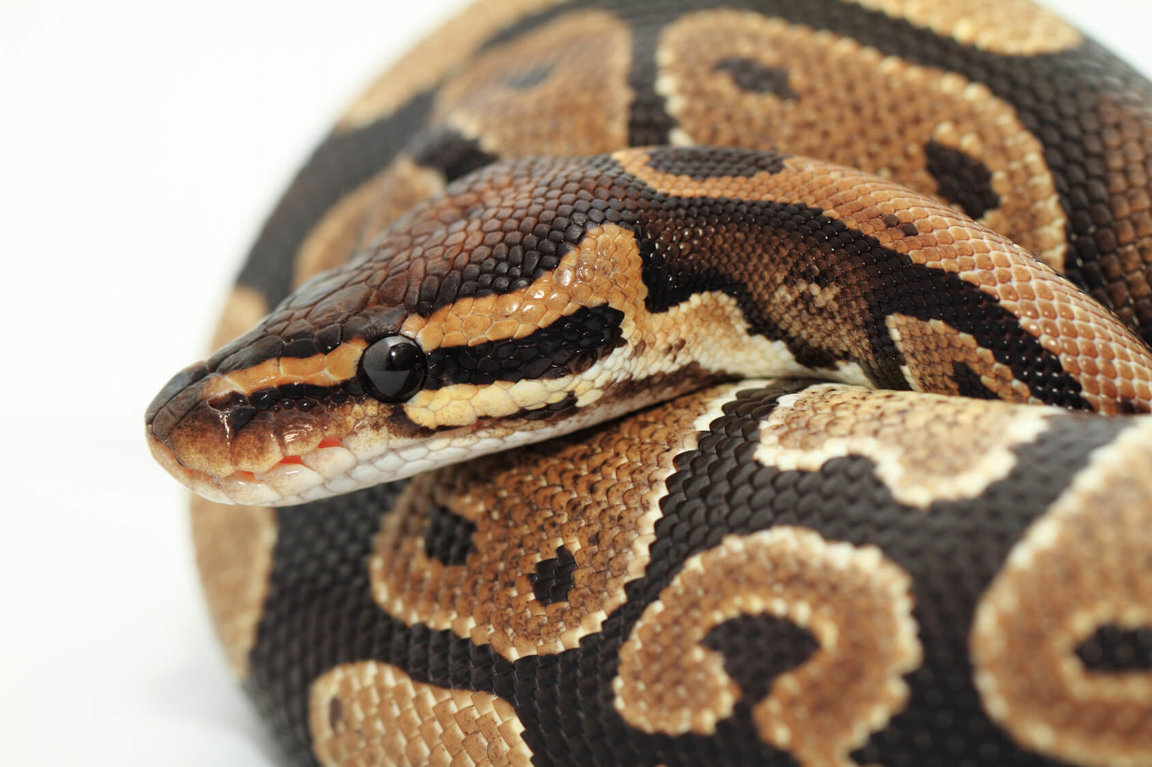
\includegraphics[height=\paperheight]{logos/Wild_Python.jpg}\hfil}\vfil}
	}
	\frame{
		\frametitle{Why use Workflow Managers?}
		\begin{mdframed}[tikzsetting={draw=white,fill=white,fill opacity=0.8,
				line width=0pt},backgroundcolor=none,leftmargin=0,
			rightmargin=150,innertopmargin=4pt,roundcorner=10pt]
			\tableofcontents[currentsection,sections={1-4},hideothersubsections]
		\end{mdframed}
	    \vfill\vspace{12mm}\hfil \hfill{\tiny own creating with Stable Diffusion}
	}
}

%%%%%%%%%%%%%%%%%%%%%%%%%%%%%%%%%%%%%%%%%%%%%%%%%%%%%%%%%%%%%%%%%%%%%%%%%%%%%%%%
\begin{frame}
  \frametitle{What is this about?}
   \begin{question}[Questions]
   	 \begin{itemize}
        \item I can code everything! Can I?
        \item What is the benefit of a workflow system?
        \item What distinguishes a workflow system from a ``pipeline''?
     \end{itemize}
   \end{question}
   \begin{docs}[Objectives]
   	  \begin{enumerate}
         \item Introducing workflow management sytems -- particularly \Snakemake!
      \end{enumerate}
   \end{docs}
\end{frame}  

%%%%%%%%%%%%%%%%%%%%%%%%%%%%%%%%%%%%%%%%%%%%%%%%%%%%%%%%%%%%%%%%%%%%%%%%%%%%%%%%
\begin{frame}
  \frametitle{Data Analysis}
  \centering
  \begin{onlyenv}<1| handout:0>
    \begin{tikzpicture}
      \path[use as bounding box] (0.7,0) rectangle (12,8);
      \node[inner sep=0pt] (analysis_1) at (5,5.5)
         {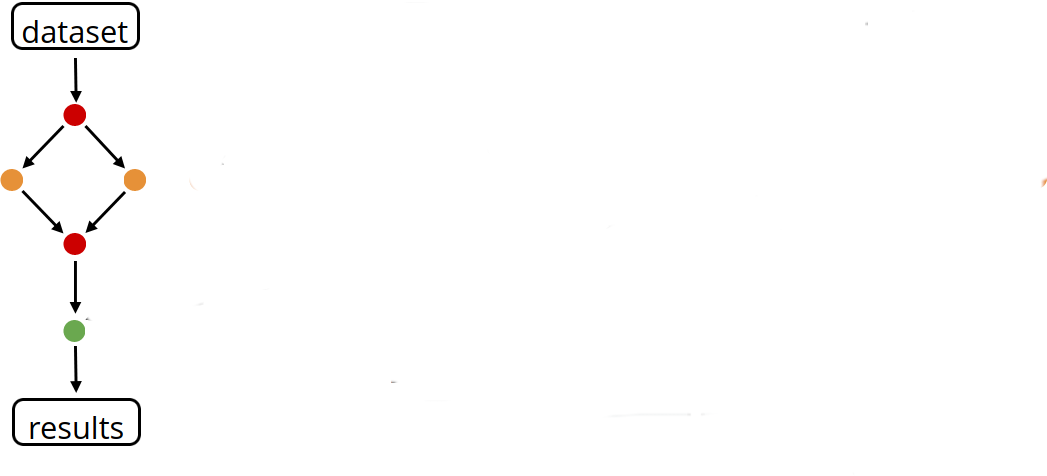
\includegraphics[width=0.7\textwidth]{Snakemake/analysis_1.png}};   
      \node at (7, 3.5) %[below=-0.4cm of analysis_1, xshift=2.7cm] at (current page.center)
         {
\includegraphics[width=0.45\textwidth]{Snakemake/phd_left.png}};
      \node at (6, 1) {\begin{minipage}{0.75\textwidth}\footnotesize
                        Idea from the official \lhref{https://slides.com/johanneskoester/snakemake-tutorial}{\Snakemake} course (with permission), image from \lhref{https://phdcomics.com/comics.php}{PhD comics}.
                       \end{minipage}
      };
    \end{tikzpicture}    
  \end{onlyenv}
  
  \begin{onlyenv}<2| handout:1>
    \begin{tikzpicture}
      \path[use as bounding box] (0.7,0) rectangle (12,8);
      \node[inner sep=0pt] (analysis_full) at (5,5.5)
         {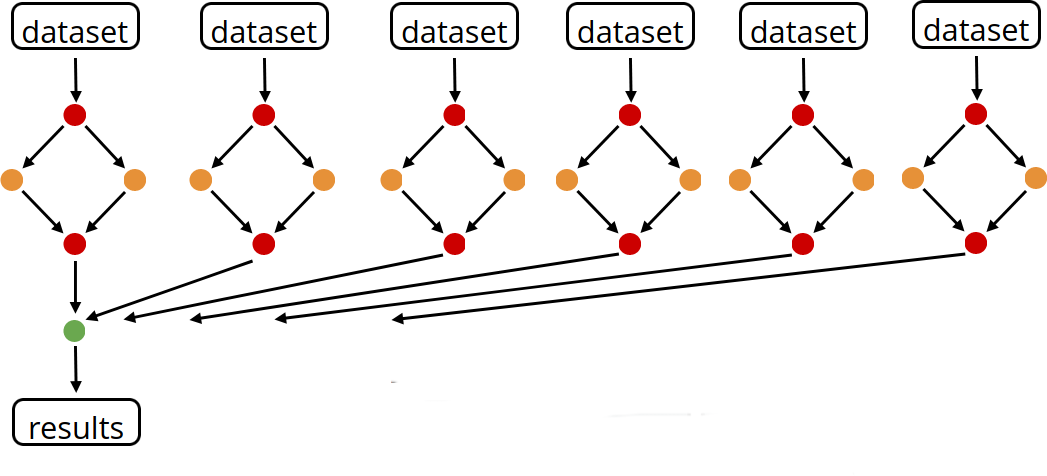
\includegraphics[width=0.7\textwidth]{Snakemake/analysis_full.png}};   
      \node at (7,3.5) % [below=-0.4cm of analysis_full, xshift=2.7cm]
         {
\includegraphics[width=0.45\textwidth]{Snakemake/phd_full.png}};
      \node at (6, 1) {\begin{minipage}{0.75\textwidth}\footnotesize
                        Idea from the official \lhref{https://slides.com/johanneskoester/snakemake-tutorial}{\Snakemake} course (with permission), image from \lhref{https://phdcomics.com/comics.php}{PhD comics}.
                       \end{minipage}
      };
    \end{tikzpicture}
  \end{onlyenv}
\end{frame}

%%%%%%%%%%%%%%%%%%%%%%%%%%%%%%%%%%%%%%%%%%%%%%%%%%%%%%%%%%%%%%%%%%%%%%%%%%%%%%%%
\begin{frame}
  \frametitle{Goals of Reproducibility}
  \Huge
  \begin{enumerate}
   \item Dispel Doubts
   \item Facilitate Further Experimentation
  \end{enumerate}
  \vfill
  \footnotesize{Idea from \lhref{https://elephly.net/downies/2023-dfn-slides.pdf}{DFN slides}.}
\end{frame}

%%%%%%%%%%%%%%%%%%%%%%%%%%%%%%%%%%%%%%%%%%%%%%%%%%%%%%%%%%%%%%%%%%%%%%%%%%%%%%%%
\begin{frame}
  \frametitle{Reproducible Data Analysis}
  \centering
  \begin{onlyenv}<1| handout:0>
    \begin{tikzpicture}
      \path[use as bounding box] (0.7,0) rectangle (12,8);
      \node at (5.5, 5) {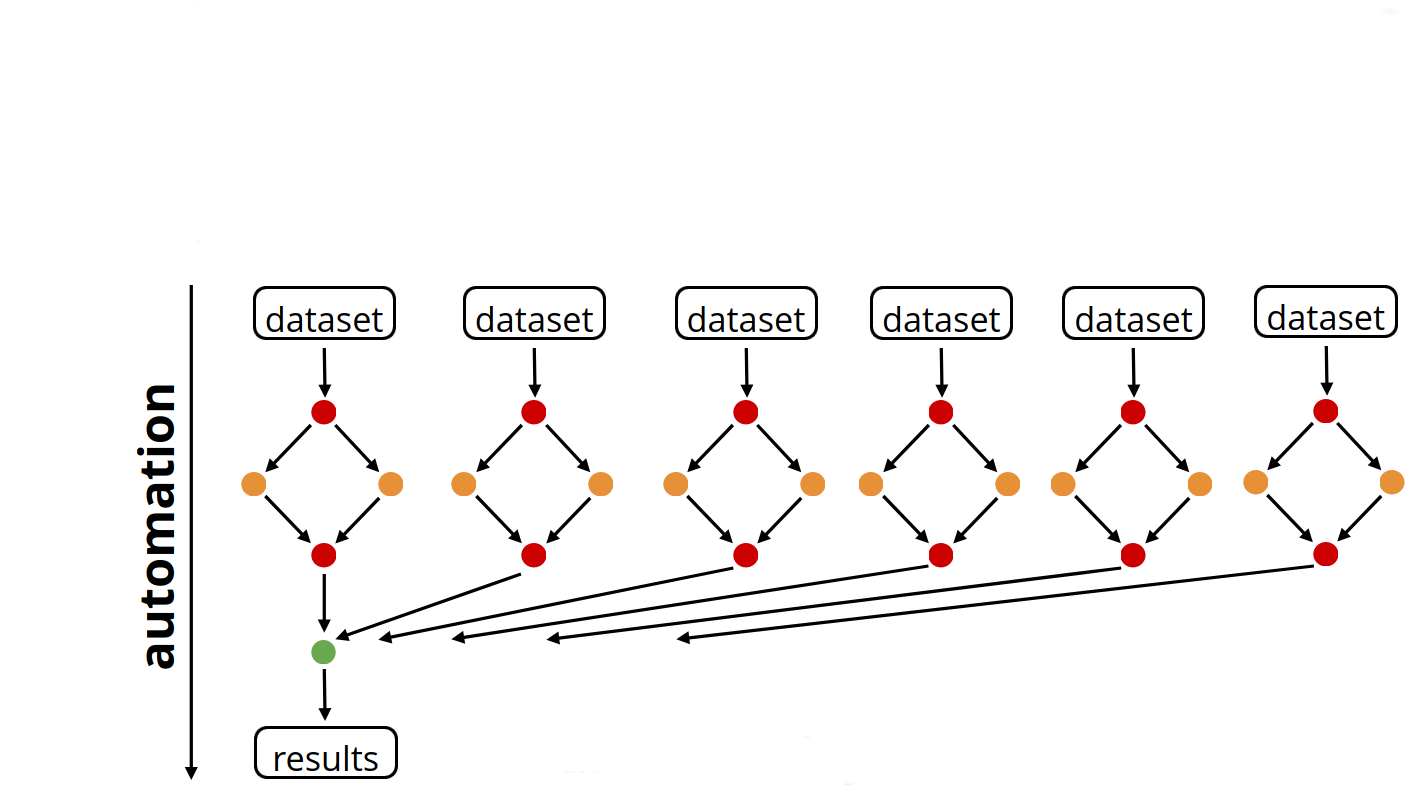
\includegraphics[width=0.7\textwidth]{Snakemake/automation.png}};
      \node at (8.5, 2) {\begin{minipage}{0.65\textwidth}
                             \textbf{From raw data to final figures:}
                             \begin{itemize}
                                \item \textbf{document} parameters, tools, versions
                                \item \textbf{execute} without manual intervention
                              \end{itemize}
                           \end{minipage}
                           };
    \end{tikzpicture}
  \end{onlyenv}
  \begin{onlyenv}<2| handout:0>
    \begin{tikzpicture}
      \path[use as bounding box] (0.7,0) rectangle (12,8);
      \node at (5.5, 5) {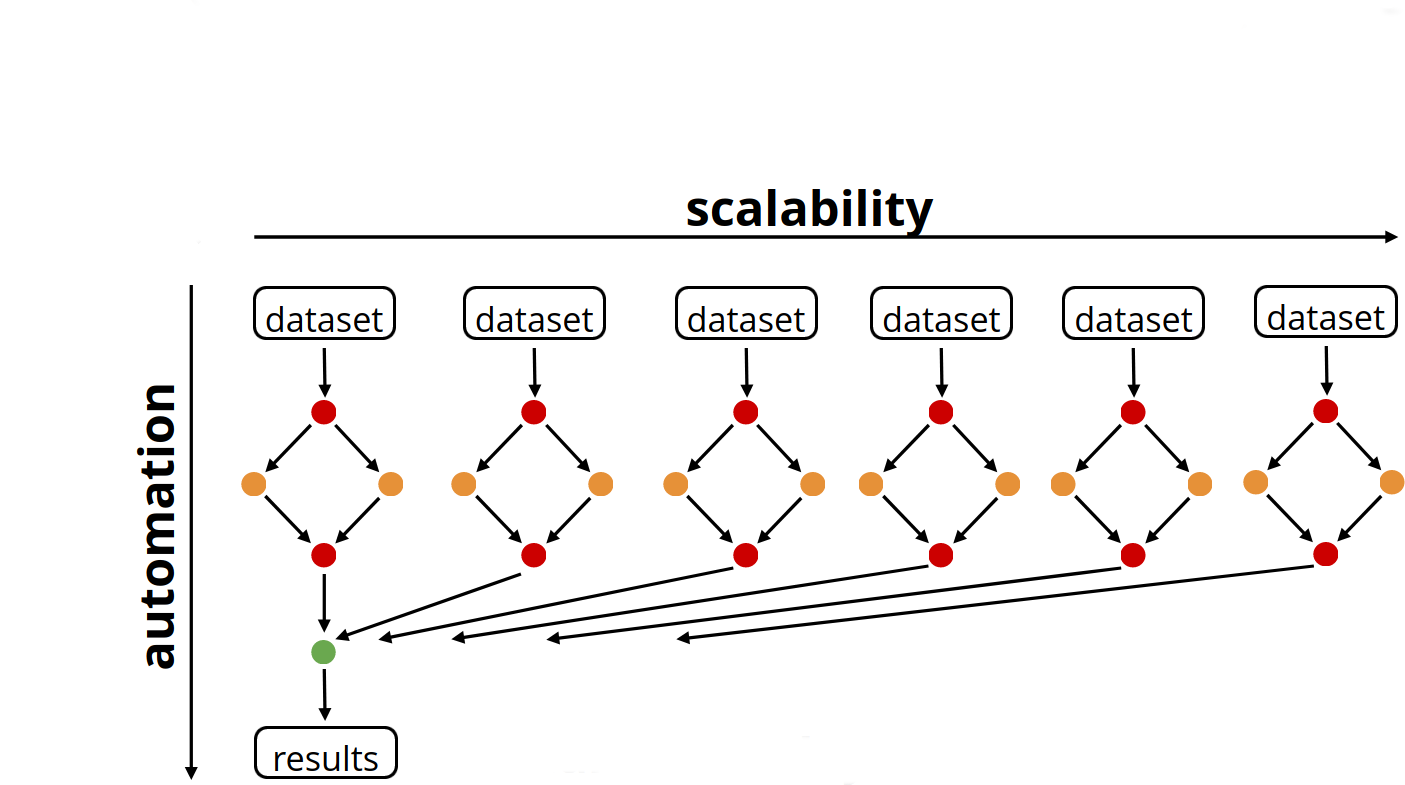
\includegraphics[width=0.7\textwidth]{Snakemake/scalability.png}};
      \node at (8.5, 2) {\begin{minipage}{0.65\textwidth}
                             \textbf{Handle parallelization:}
                             \begin{itemize}
                                \item execute for tens of thousands of datasets
                                \item efficiently use any computing platform
                              \end{itemize}
                           \end{minipage}
                           };
    \end{tikzpicture}
  \end{onlyenv}
  \begin{onlyenv}<3| handout:1>
    \begin{tikzpicture}
      \path[use as bounding box] (0.7,0) rectangle (12,8);
      \node at (5.5, 5) {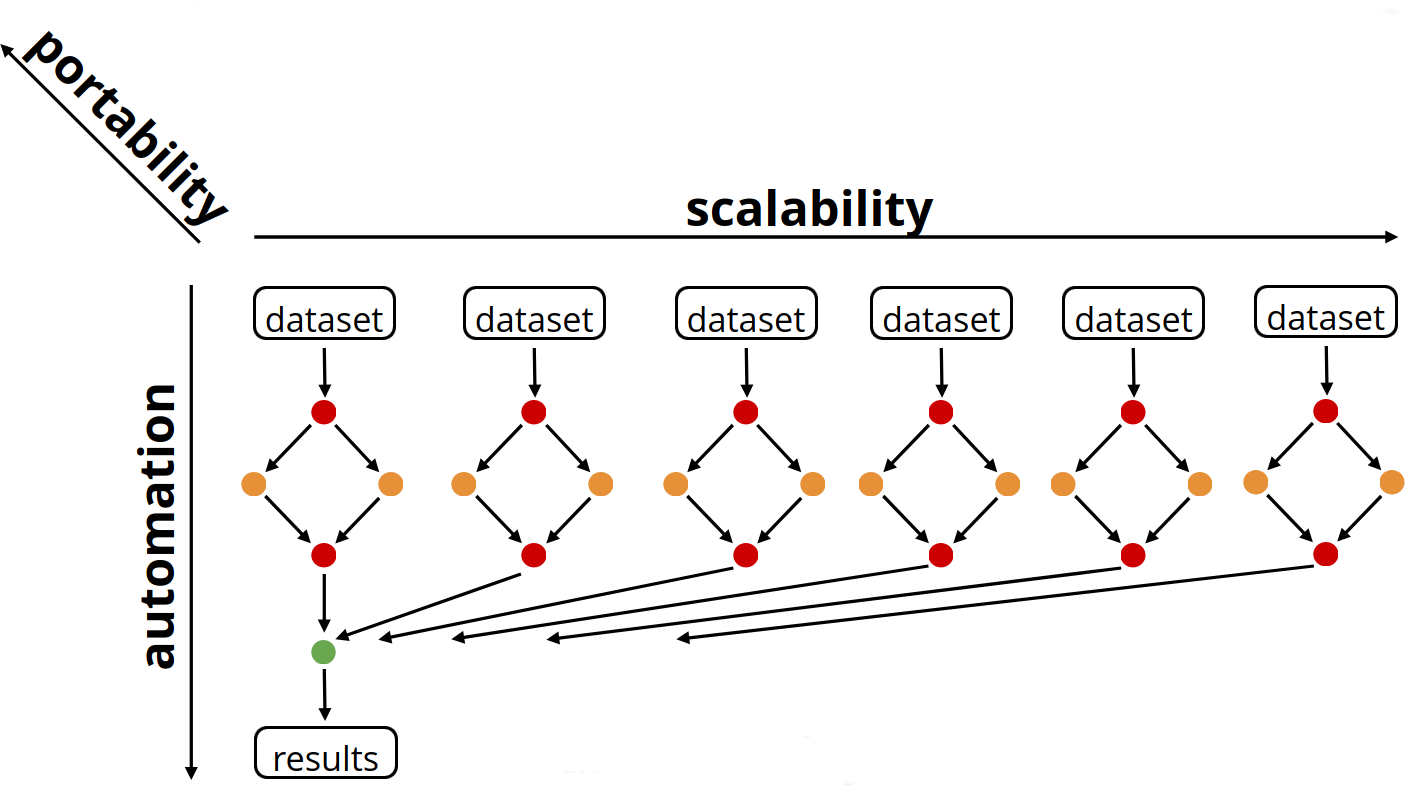
\includegraphics[width=0.7\textwidth]{Snakemake/portability.png}};
      \node at (8.5, 2) {\begin{minipage}{0.65\textwidth}
                             \textbf{Handle deployment:}\newline
                             be able to easily execute analyses on a different system/platform/infrastructure
                           \end{minipage}
                           };
    \end{tikzpicture}
  \end{onlyenv}
\end{frame}

%%%%%%%%%%%%%%%%%%%%%%%%%%%%%%%%%%%%%%%%%%%%%%%%%%%%%%%%%%%%%%%%%%%%%%%%%%%%%%%%
\begin{frame}
  \frametitle{Beyond Reproducibility}
  \begin{onlyenv}<1| handout:0>
    \begin{figure}
      \centering
      
\includegraphics[width=0.85\textwidth]{Snakemake/reproducibility_only.png}
    \end{figure}
  \end{onlyenv}
  \begin{onlyenv}<2| handout:0>
    \begin{figure}
      \centering
      
\includegraphics[width=0.85\textwidth]{Snakemake/reproducibility_empty.png}
    \end{figure}
  \end{onlyenv}
  \begin{onlyenv}<3| handout:0>
    \begin{figure}
      \centering
      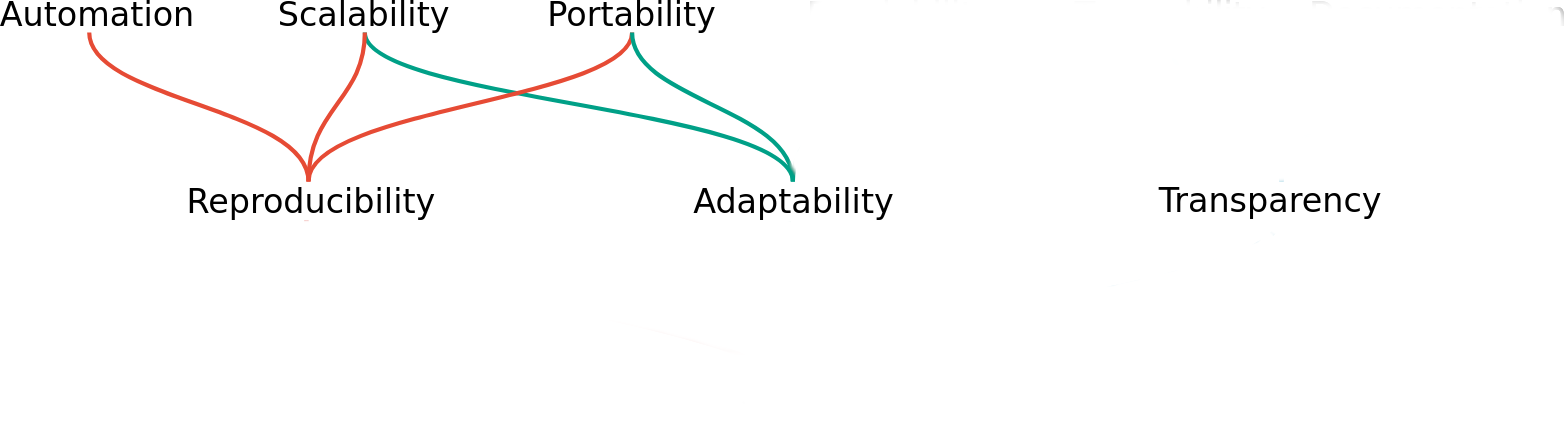
\includegraphics[width=0.85\textwidth]{Snakemake/reproducibility_left.png}
    \end{figure}
  \end{onlyenv}
    \begin{onlyenv}<4| handout:1>
      \begin{figure}
        \centering
        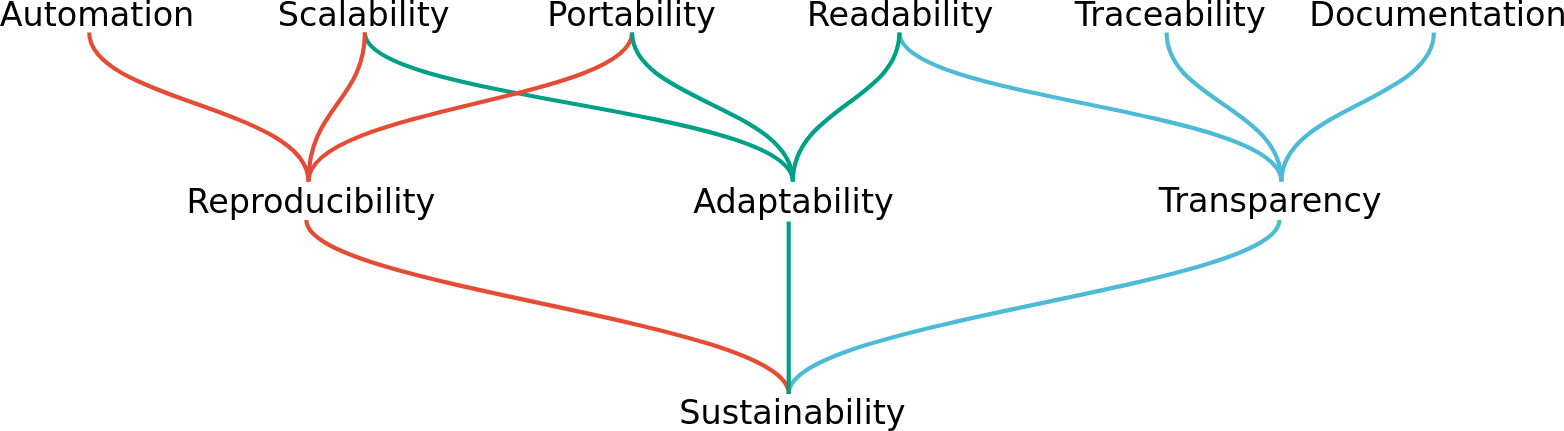
\includegraphics[width=0.85\textwidth]{Snakemake/reproducibility_full.png}
      \end{figure}
  \end{onlyenv}
  \footnotesize{\lhref{https://doi.org/10.12688/f1000research.29032.2}{From the official \Snakemake-paper.}}
\end{frame}

%%%%%%%%%%%%%%%%%%%%%%%%%%%%%%%%%%%%%%%%%%%%%%%%%%%%%%%%%%%%%%%%%%%%%%%%%%%%%%%%
\begin{frame}
    \frametitle{\Snakemake}
    \begin{figure}
        \centering
        \caption*{\textbf{>1.2e6} downloads since 2015\newline
            \textbf{>14} citations per week}
        
\includegraphics[width=0.6\textwidth]{Snakemake/paper_wall.png}
    \end{figure}
\end{frame}

%%%%%%%%%%%%%%%%%%%%%%%%%%%%%%%%%%%%%%%%%%%%%%%%%%%%%%%%%%%%%%%%%%%%%%%%%%%%%%%%
\begin{frame}
    \frametitle{The \Snakemake{} Catalogue}
    \begin{columns}
        \begin{column}{0.5\textwidth}
            \begin{itemize}[<+->]
                \item Extremely feature rich: \lhref{https://snakemake.github.io/snakemake-workflow-catalog/}{over 2000 workflows}
                \item Almost 400 standardized workflows ready to use (meaning: well documented and with automatic deployment)
                \item Cluster batch systems are supported (and support for various cloud systems, too)
            \end{itemize}
        \end{column}
        \begin{column}{0.5\textwidth}
            \begin{figure}
                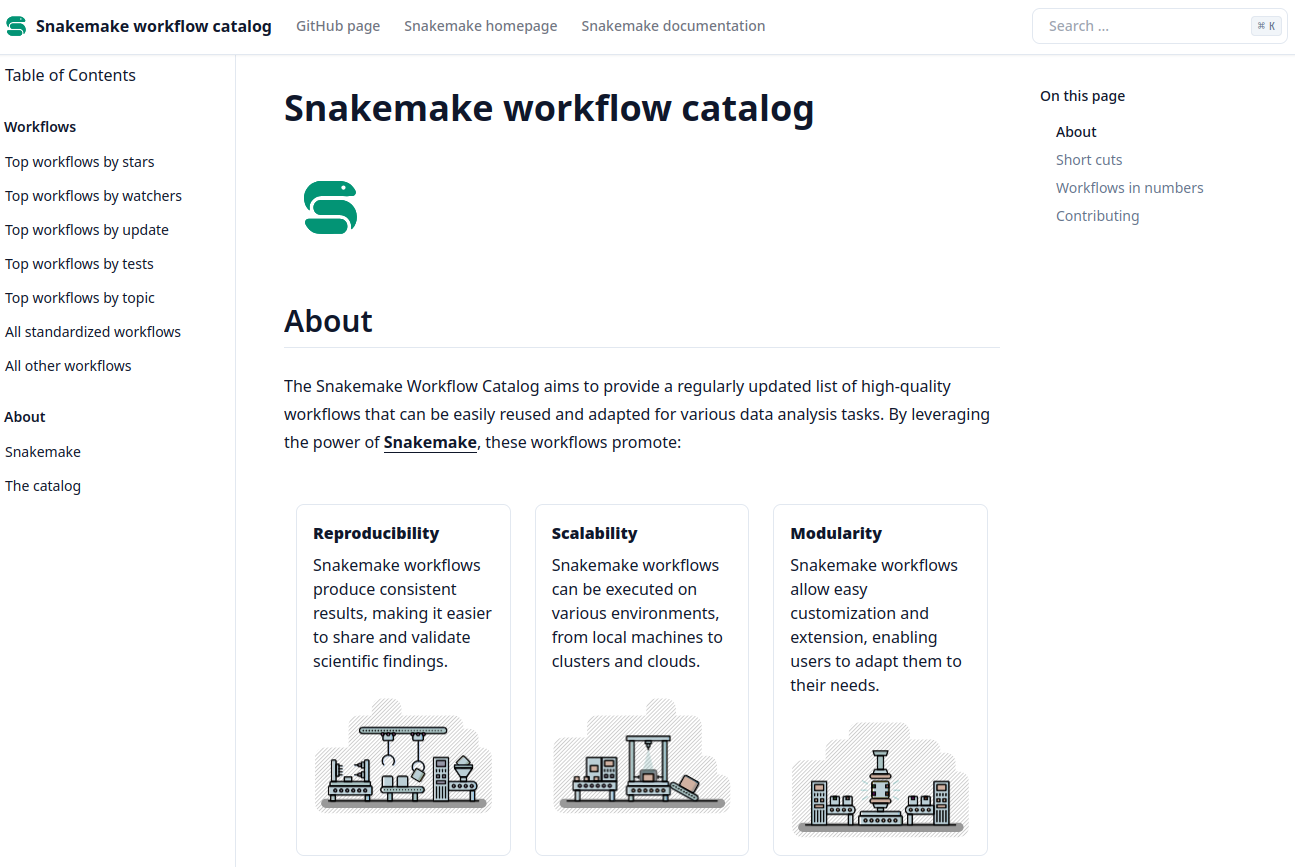
\includegraphics[width=\textwidth]{Snakemake/Snakemake_Workflow_Catalog.png}
                \caption*{Screenshot of the Workflow Catalogue}
            \end{figure}
        \end{column}
    \end{columns}
\end{frame}

%%%%%%%%%%%%%%%%%%%%%%%%%%%%%%%%%%%%%%%%%%%%%%%%%%%%%%%%%%%%%%%%%%%%%%%%%%%%%%%%
\begin{frame}
	\frametitle{A simple real-life Workflow}
	\begin{onlyenv}<1| handout:0>
	\begin{figure}
		\centering
		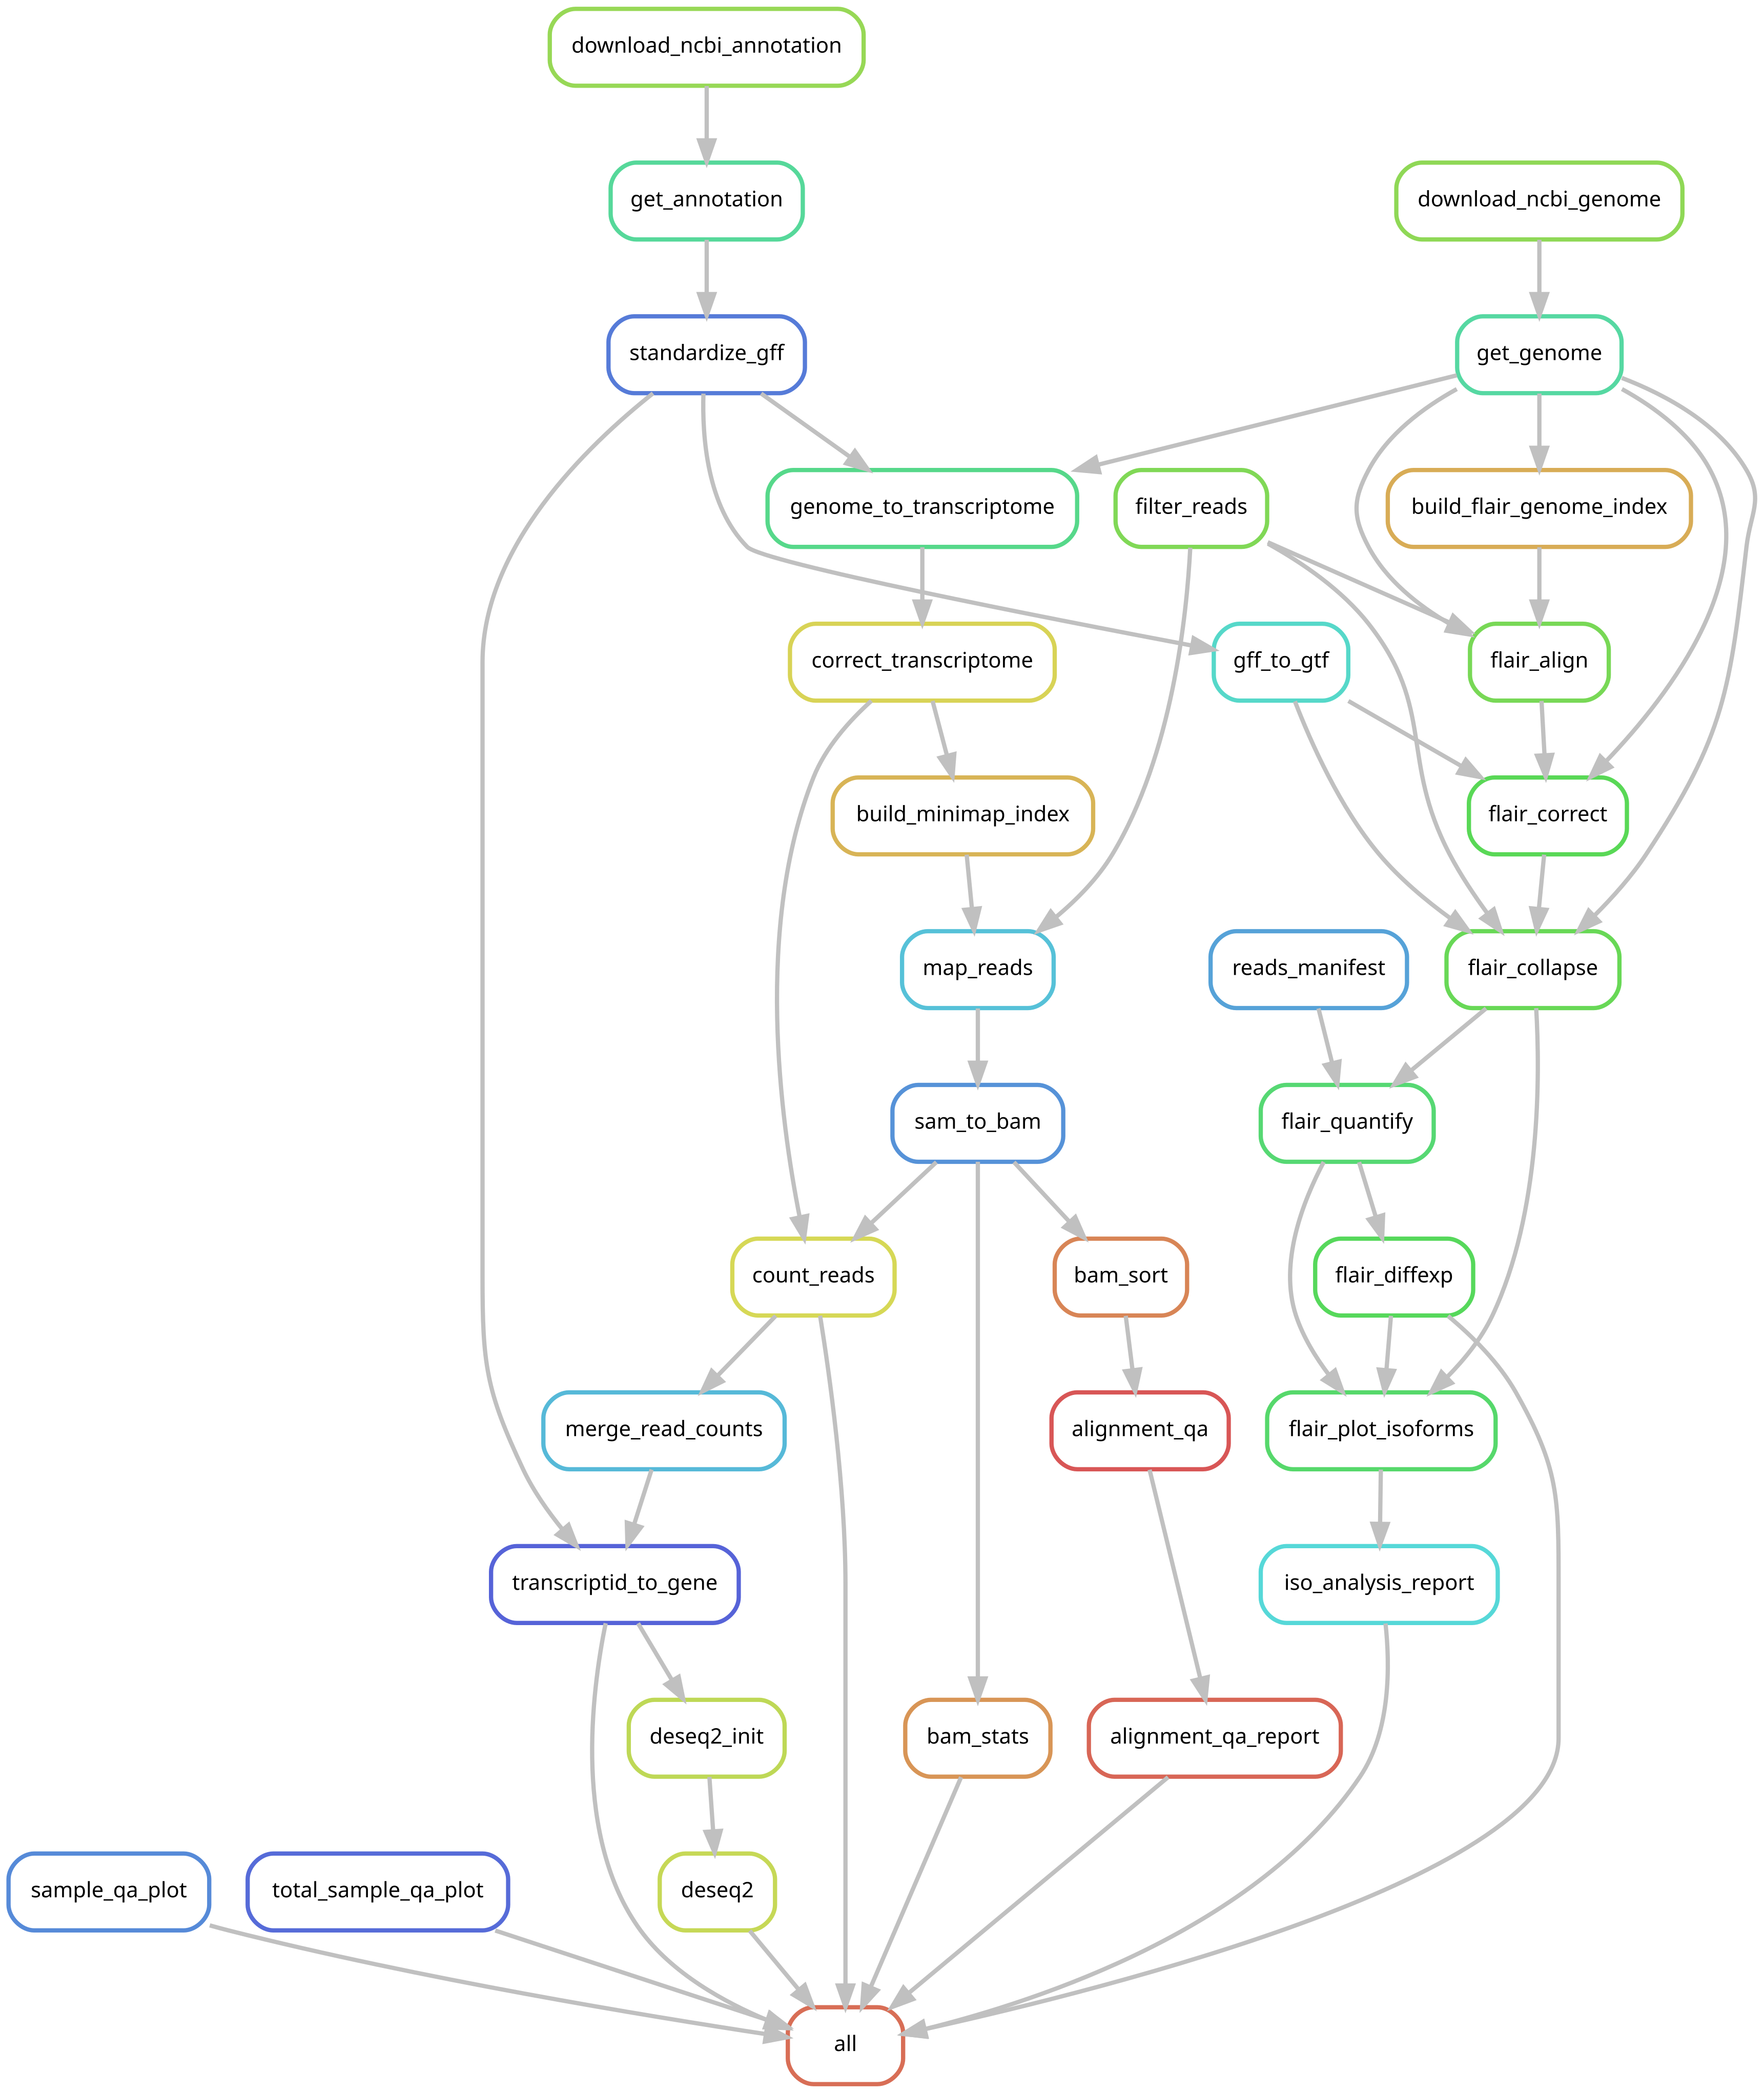
\includegraphics[width=0.5\textwidth]{workflows/rulegraph.png}
		The "rulegraph"
	\end{figure}
	\end{onlyenv}
	\begin{onlyenv}<2| handout:0>
	\begin{figure}
		\centering
		
\includegraphics[width=0.85\textwidth]{workflows/dag.png}\\
		The "DAG" (directed acyclic graph) incl. all sample rules
	\end{figure}
	\end{onlyenv}
\end{frame}

%%%%%%%%%%%%%%%%%%%%%%%%%%%%%%%%%%%%%%%%%%%%%%%%%%%%%%%%%%%%%%%%%%%%%%%%%%%%%%%%
\begin{frame}
	\frametitle{The Tutorial Workflow}
	\begin{columns}
		\begin{column}{0.5\textwidth}
			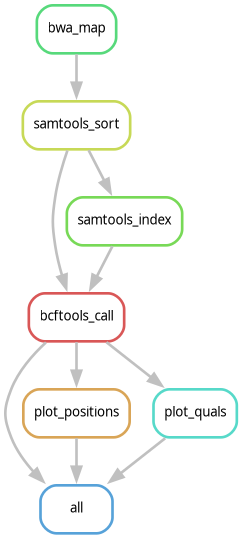
\includegraphics[width=0.45\textwidth]{workflows/rulegraph_lifescience.png}\\
			The full tutorial rulegraph.
		\end{column}
		\begin{column}{0.5\textwidth}
			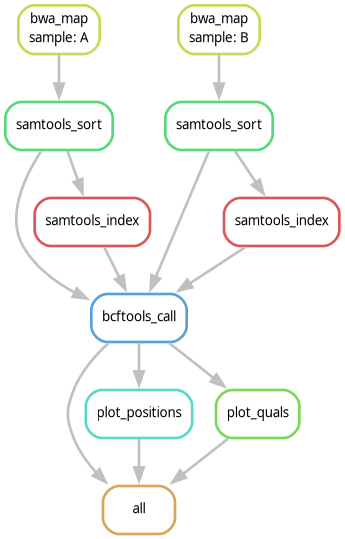
\includegraphics[width=0.65\textwidth]{workflows/dag_full_lifescience.png}\\
			The full tutorial DAG.
		\end{column}
	\end{columns}
\end{frame}

%%%%%%%%%%%%%%%%%%%%%%%%%%%%%%%%%%%%%%%%%%%%%%%%%%%%%%%%%%%%%%%%%%%%%%%%%%%%%%%%
\begin{frame}
	\centering
    Here followed\newline
	{\Huge A DEMO}\newline
    of the tutorial workflow.\newline\\
    Requiring some imagination of what a BIG workflow might be capable of.
\end{frame}

%%%%%%%%%%%%%%%%%%%%%%%%%%%%%%%%%%%%%%%%%%%%%%%%%%%%%%%%%%%%%%%%%%%%%%%%%%%%%%%%
%%%%%%%%%%%%%%%%%%%%%%%%%%%%%%%%%%%%%%%%%%%%%%%%%%%%%%%%%%%%%%%%%%%%%%%%%%%%%%%%%
\section{Snakemake  Reports}
{   
    \usebackgroundtemplate{
        \vbox to \paperheight{\vfil\hbox to \paperwidth{\hfil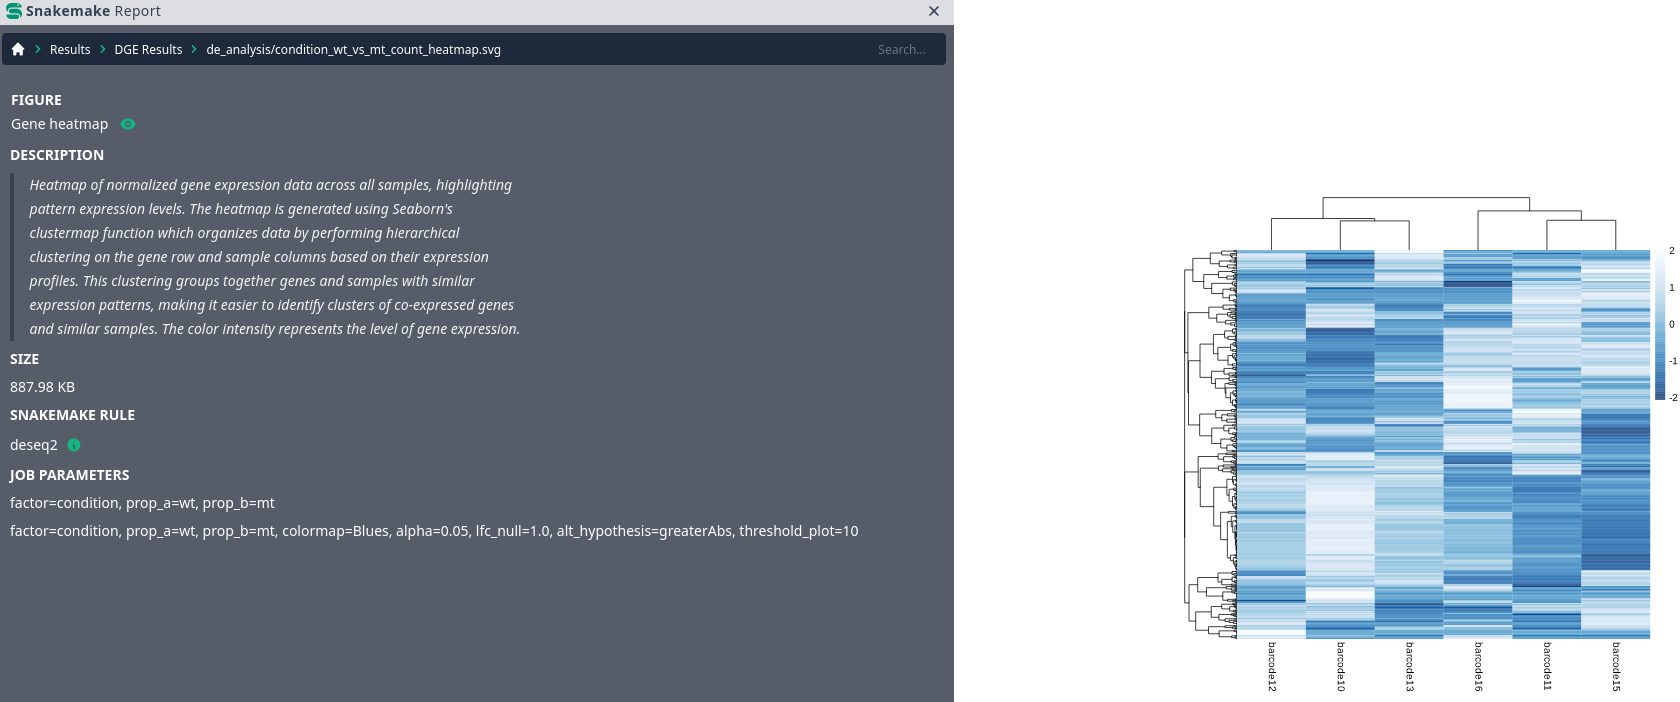
\includegraphics[width=\paperwidth]{reports/snakemake_html_workflow_report.png}\hfil}\vfil}
    }
    \frame{
        \frametitle{\Snakemake Reports}
        \begin{mdframed}[tikzsetting={draw=white,fill=white,fill opacity=0.8,
                line width=0pt},backgroundcolor=none,leftmargin=0,
            rightmargin=150,innertopmargin=4pt,roundcorner=10pt]
            \tableofcontents[currentsection,sections={1-4},hideothersubsections]
        \end{mdframed}
        \vfill\vspace{16mm}\hfil \hfill{\tiny Screenshot --of a \Snakemake HTML report}
    }
}


%%%%%%%%%%%%%%%%%%%%%%%%%%%%%%%%%%%%%%%%%%%%%%%%%%%%%%%%%%%%%%%%%%%%%%%%%%%%%%%%
\begin{frame}[fragile]
	\frametitle{How does a \Snakemake Report look like?}
    \begin{figure}[c]
        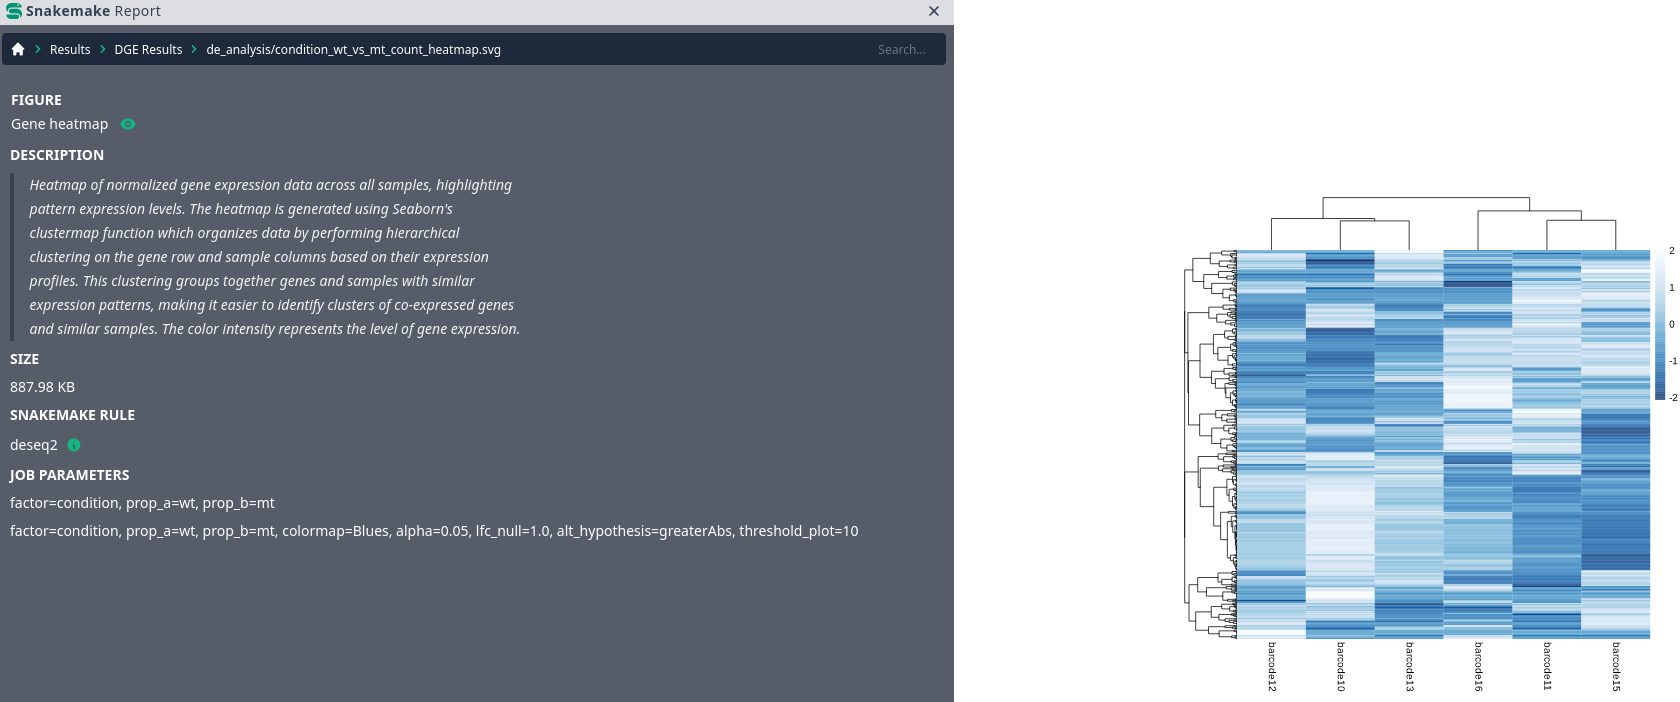
\includegraphics[width=0.9\textwidth]{reports/snakemake_html_workflow_report.png}
        \caption*{
            \\ This is a HTML report of the workflow presented earlier. Designed for teaching. Download from \url{https://doi.org/10.5281/zenodo.18860872}. (The nanopub for it is \lhref{https://w3id.org/np/RApK8IUY9KJJkFoasvMJhPQQtT8VvN0IQ__hAxKOeeIuk}{\altverb{RApK8IUY9KJJkFoasvMJhPQQtT8VvN0IQ__hAxKOeeIuk}}.)\\
            \Snakemake's HTML reports are designed to give all meta-information and publication-ready figures!
        }
    \end{figure}
\end{frame}

%%%%%%%%%%%%%%%%%%%%%%%%%%%%%%%%%%%%%%%%%%%%%%%%%%%%%%%%%%%%%%%%%%%%%%%%%%%%%%%%
\begin{frame}
    \centering
    {\Huge A DEMO of Reports}
    \newline Here, we did a little demo of workflow reports.
    \\
    Participants were asked to download and browse the html report.
\end{frame}

%%%%%%%%%%%%%%%%%%%%%%%%%%%%%%%%%%%%%%%%%%%%%%%%%%%%%%%%%%%%%%%%%%%%%%%%%%%%%%%%
\begin{frame}[fragile]
	\frametitle{Snakemake Reports}
	To create a html report
	\begin{lstlisting}[language=Bash, style=Shell]
snakemake ... --report
    \end{lstlisting}
    \begin{block}
        This gives you a HTML report like the one we have seen (if the workflow is programmed to do so, else just a basic HTML report). To 
    \end{block}
\end{frame}

%%%%%%%%%%%%%%%%%%%%%%%%%%%%%%%%%%%%%%%%%%%%%%%%%%%%%%%%%%%%%%%%%%%%%%%%%%%%%%%%
\begin{frame}
    \frametitle{Steps needed to register Workflow MetaData}
    To create a nanopub report:
    \begin{itemize}[<+->]
        \item First install the plugin (next).
        \item Register with the Nanopub framework (next).
        \item Register your workflow with Nanopubs using the \Snakemake nanopub reporter plugin, \textit{because only then a full connection between workflow and report can be made} (our hands on part - the end).
        \item Learn how to create a knowledge graph including the \textbf{workflow}, its \textbf{configuration}, the \textbf{dataset} you have been working with, and the final \textbf{report} (our hands on part - the very end) 
    \end{itemize}
\end{frame}



%%%%%%%%%%%%%%%%%%%%%%%%%%%%%%%%%%%%%%%%%%%%%%%%%%%%%%%%%%%%%%%%%%%%%%%%%%%%%%%%
%%%%%%%%%%%%%%%%%%%%%%%%%%%%%%%%%%%%%%%%%%%%%%%%%%%%%%%%%%%%%%%%%%%%%%%%%%%%%%%%%
\section{Nanopub Onboarding}
{   
	\usebackgroundtemplate{
		\vbox to \paperheight{\vfil\hbox to \paperwidth{\hfil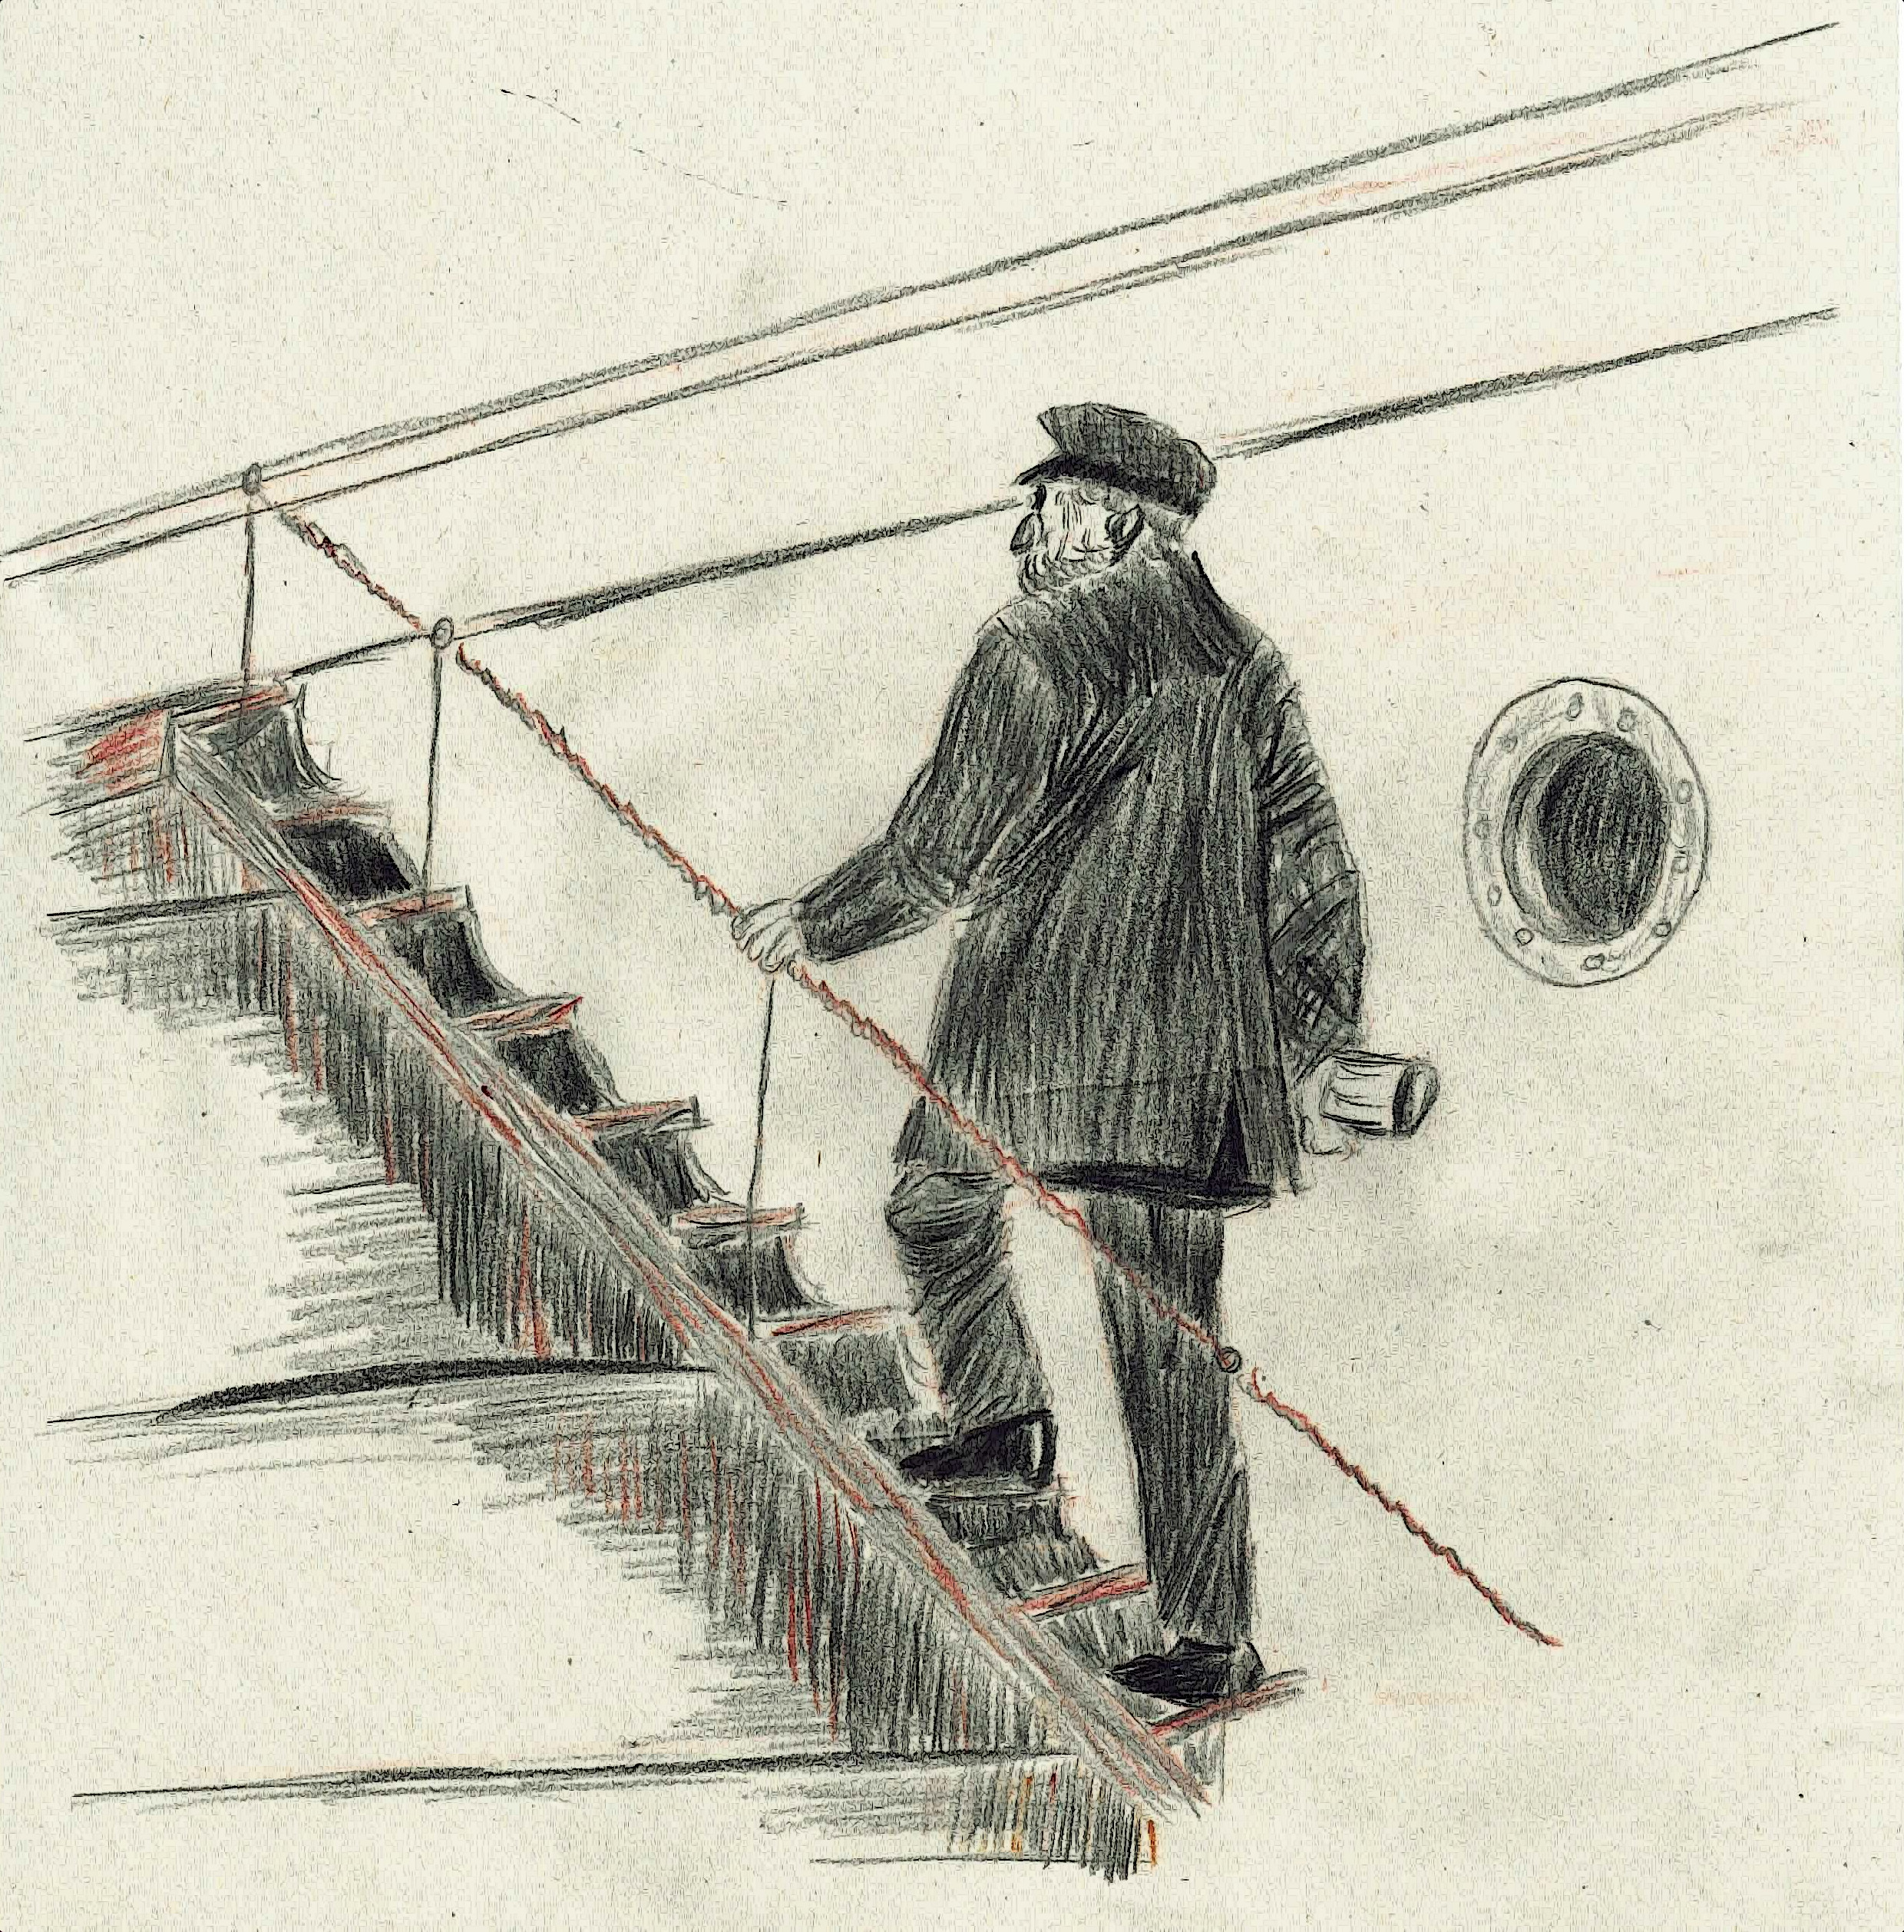
\includegraphics[width=\paperwidth]{humor/onboarding_cartoon.jpg}\hfil}\vfil}
	}
	\frame{
		\frametitle{Register with the Nanopub}
		\begin{mdframed}[tikzsetting={draw=white,fill=white,fill opacity=0.8,
				line width=0pt},backgroundcolor=none,leftmargin=0,
			rightmargin=150,innertopmargin=4pt,roundcorner=10pt]
			\tableofcontents[currentsection,sections={1-4},hideothersubsections]
		\end{mdframed}
		\vfill\vspace{18mm}\hfil \hfill{\tiny own sketch after "Dropping the Pilot" -- CC-BY-4.0}
	}
}

%%%%%%%%%%%%%%%%%%%%%%%%%%%%%%%%%%%%%%%%%%%%%%%%%%%%%%%%%%%%%%%%%%%%%%%%%%%%%%%% 
\frame{
  \frametitle{What is a Nanopub?}
  \begin{columns}[T]
    \column{0.3\textwidth}
       \centering
       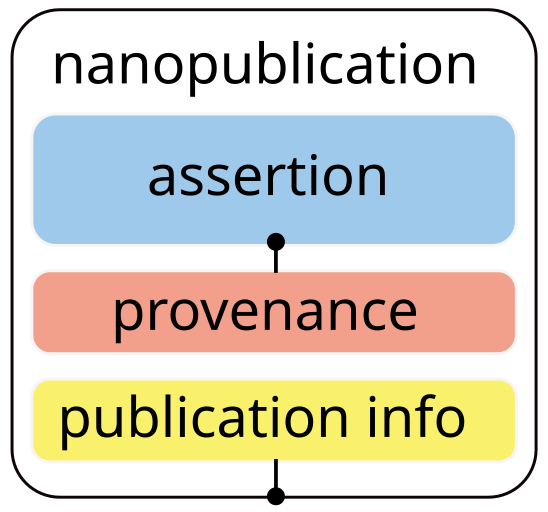
\includegraphics[width=\linewidth]{nanopub_logo.png} \\
       Think of a Nanopub as a little knowledge container.
    \column{0.7\textwidth}
       \centering
       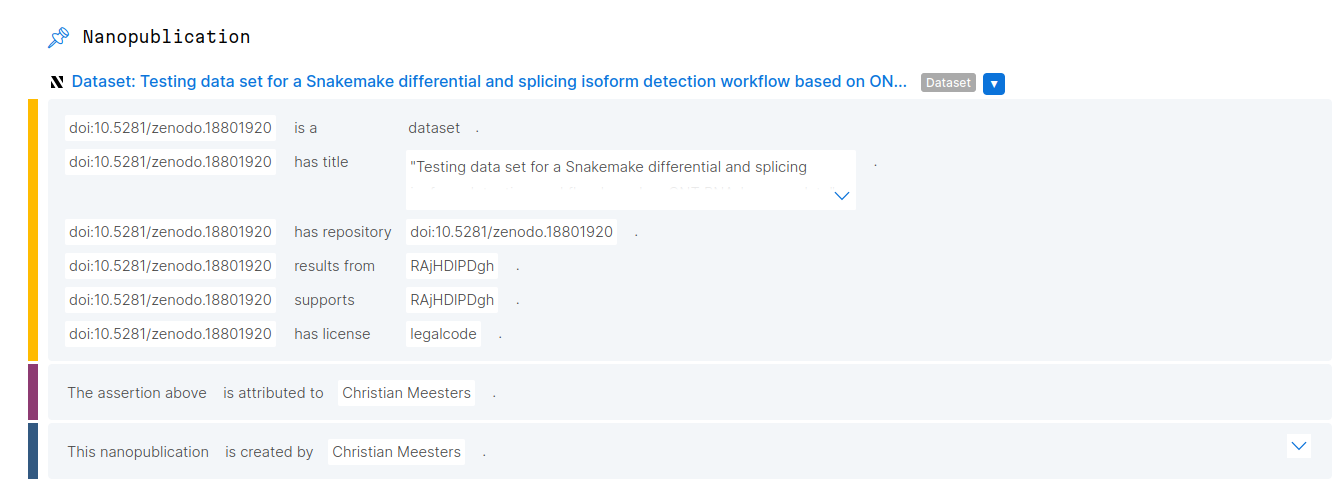
\includegraphics[width=\linewidth]{example_nanopub_dataset.png} \\
       This is an example Nanopub, a dataset description.
   \end{columns}
}
    
%%%%%%%%%%%%%%%%%%%%%%%%%%%%%%%%%%%%%%%%%%%%%%%%%%%%%%%%%%%%%%%%%%%%%%%%%%%%%%%% 
\frame{
  \frametitle{Register your account}
  \begin{columns}
      \begin{column}{0.5\textwidth}
          If you don't have an account yet, please register at
          \href{https://nanodash.knowledgepixels.com}{nanodash} using your ORCID iD.
      \end{column}
      \begin{column}{0.5\textwidth}
         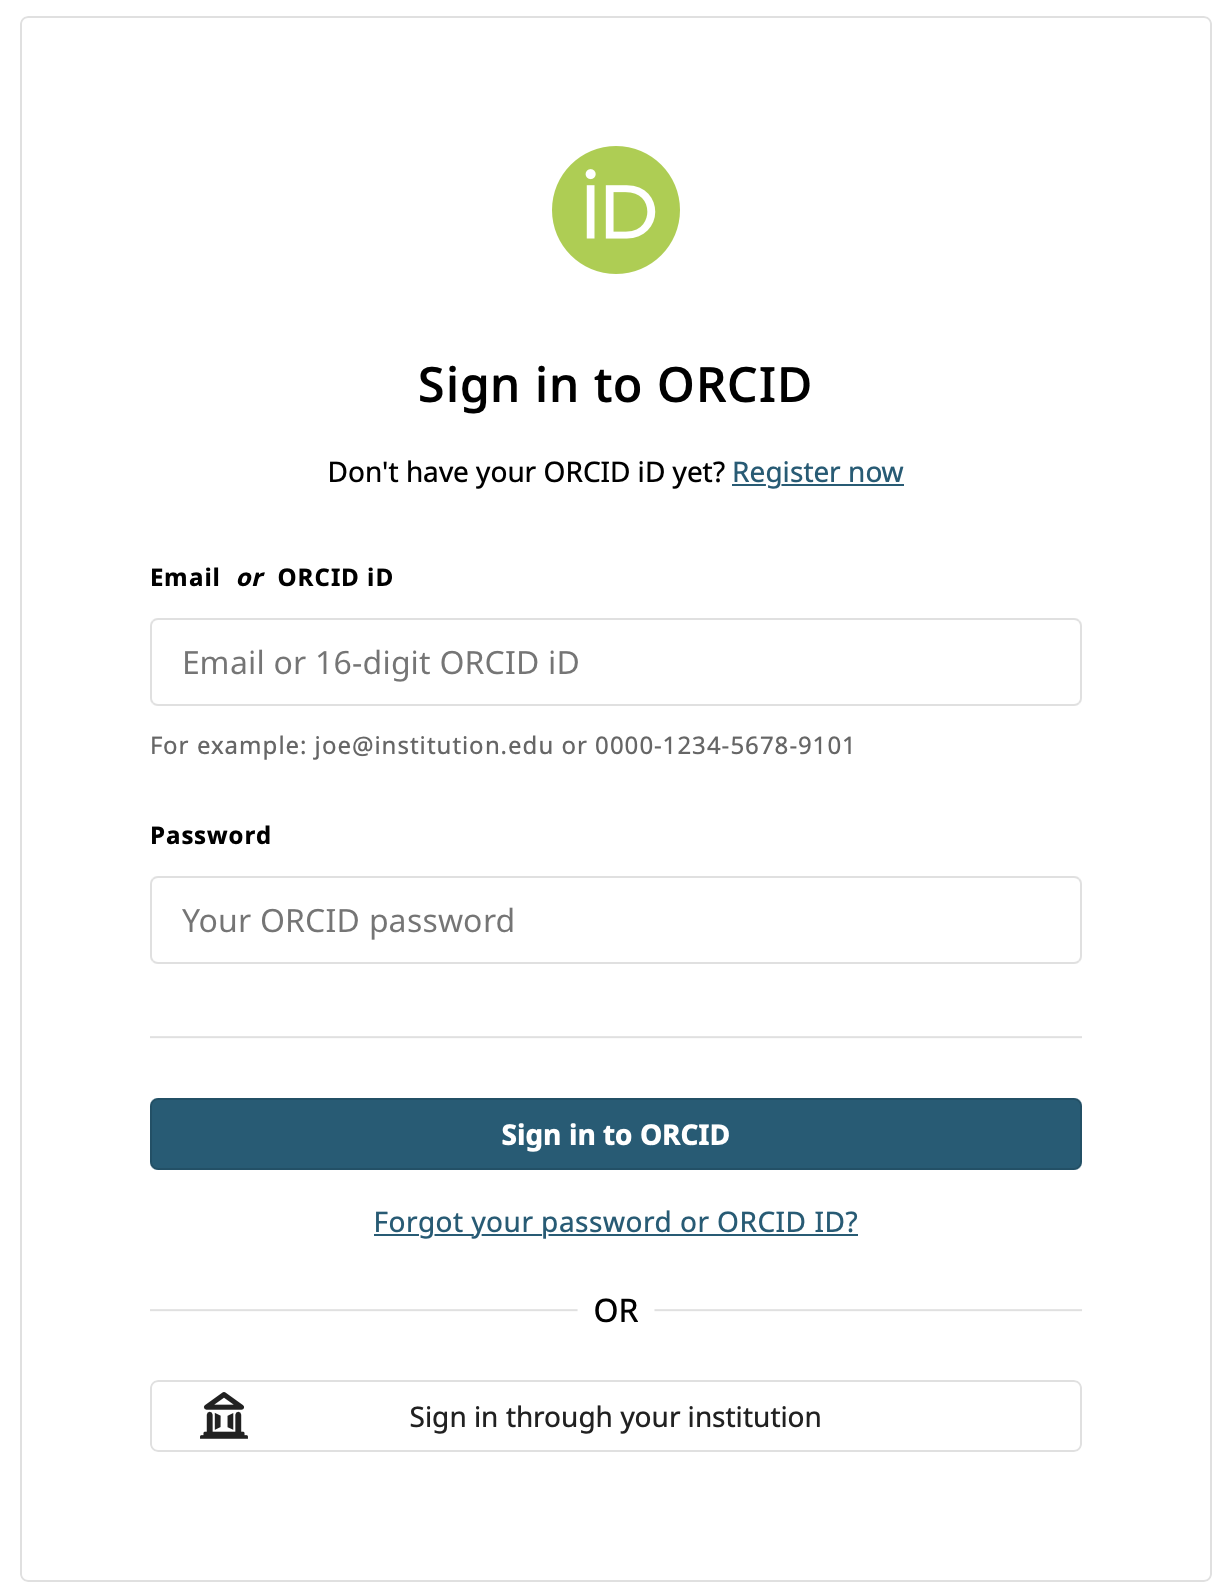
\includegraphics[width=0.9\linewidth]{register.png}
      \end{column}
  \end{columns}


  
}

%%%%%%%%%%%%%%%%%%%%%%%%%%%%%%%%%%%%%%%%%%%%%%%%%%%%%%%%%%%%%%%%%%%%%%%%%%%%%%%%  
\frame{
  \frametitle{Interlude: What is an ORCID?}
  ORCID stands for \textbf{O}pen \textbf{R}esearcher and \textbf{C}ontributor \textbf{ID}.
  \vspace{1em}
  \begin{itemize}
    \item<+-> free, unique \& persistent ID
    \item<+-> show your research interest, funding, employment and \textbf{publications} (sometimes they add automagically with Crossref)
    \item<+-> useful in research to be found:
    \begin{itemize}
       \item<+-> for agencies to look you up during proposal reviews
       \item<+-> to find colleagues (and see how actively they are engaged and in which topics)
    \end{itemize}
  \end{itemize}
}
   
%%%%%%%%%%%%%%%%%%%%%%%%%%%%%%%%%%%%%%%%%%%%%%%%%%%%%%%%%%%%%%%%%%%%%%%%%%%%%%%%  
\frame{
  \frametitle{Interlude: What is an ORCID? II}
  \begin{columns}[T]
    \begin{column}{0.25\textwidth}
      \centering
      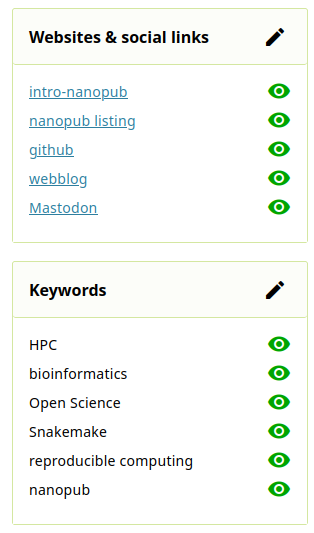
\includegraphics[width=\linewidth]{orcid_profile_links_keywords.png} \\
      Example screenshot with links and research interests.
    \end{column}
    \begin{column}{0.65\textwidth}
        \centering
        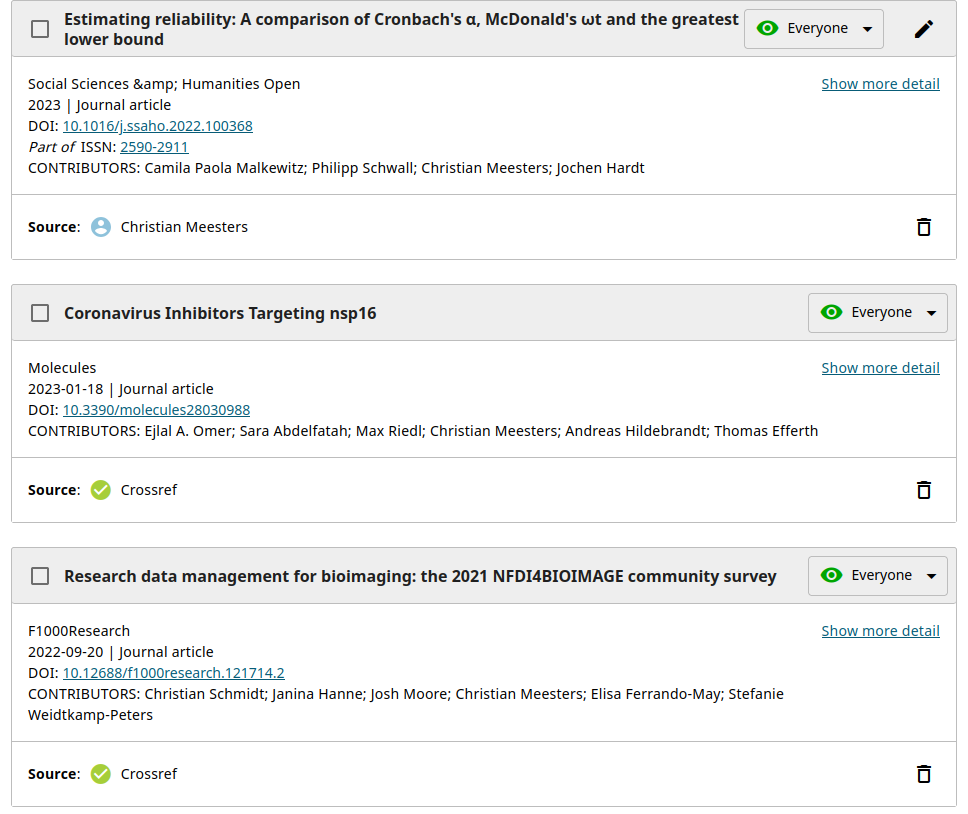
\includegraphics[width=\linewidth]{orcid_paper_examples.png} \\
        Example screenshot of papers linked in an ORCID profile.
    \end{column}
  \end{columns}
}

%%%%%%%%%%%%%%%%%%%%%%%%%%%%%%%%%%%%%%%%%%%%%%%%%%%%%%%%%%%%%%%%%%%%%%%%%%%%%%%%     
\frame{
  \frametitle{Authorise ORCID iD and enter your Nanodash account}
   \begin{columns}[T]
      \column{0.5\textwidth}
      \centering
      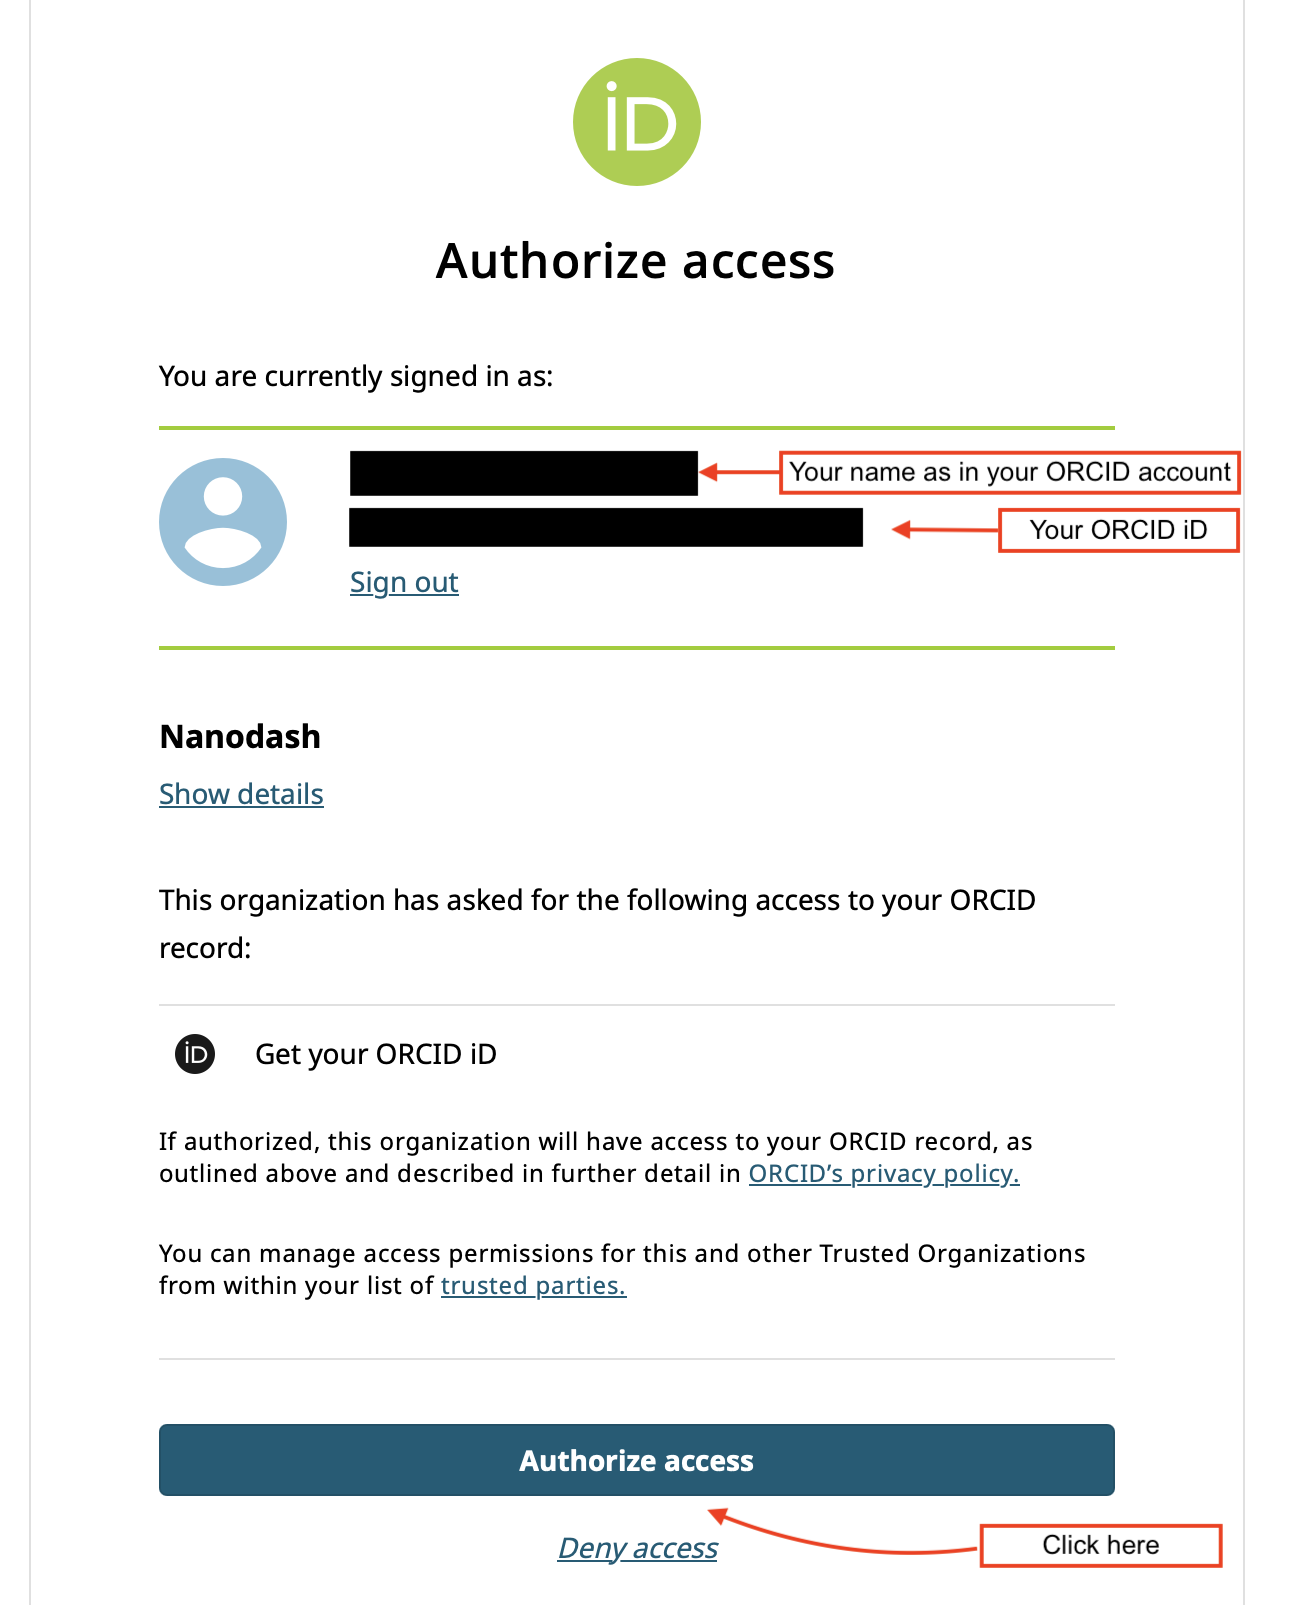
\includegraphics[width=0.9\linewidth]{authorise_orcid.png}
      \column{0.5\textwidth}
      \centering
      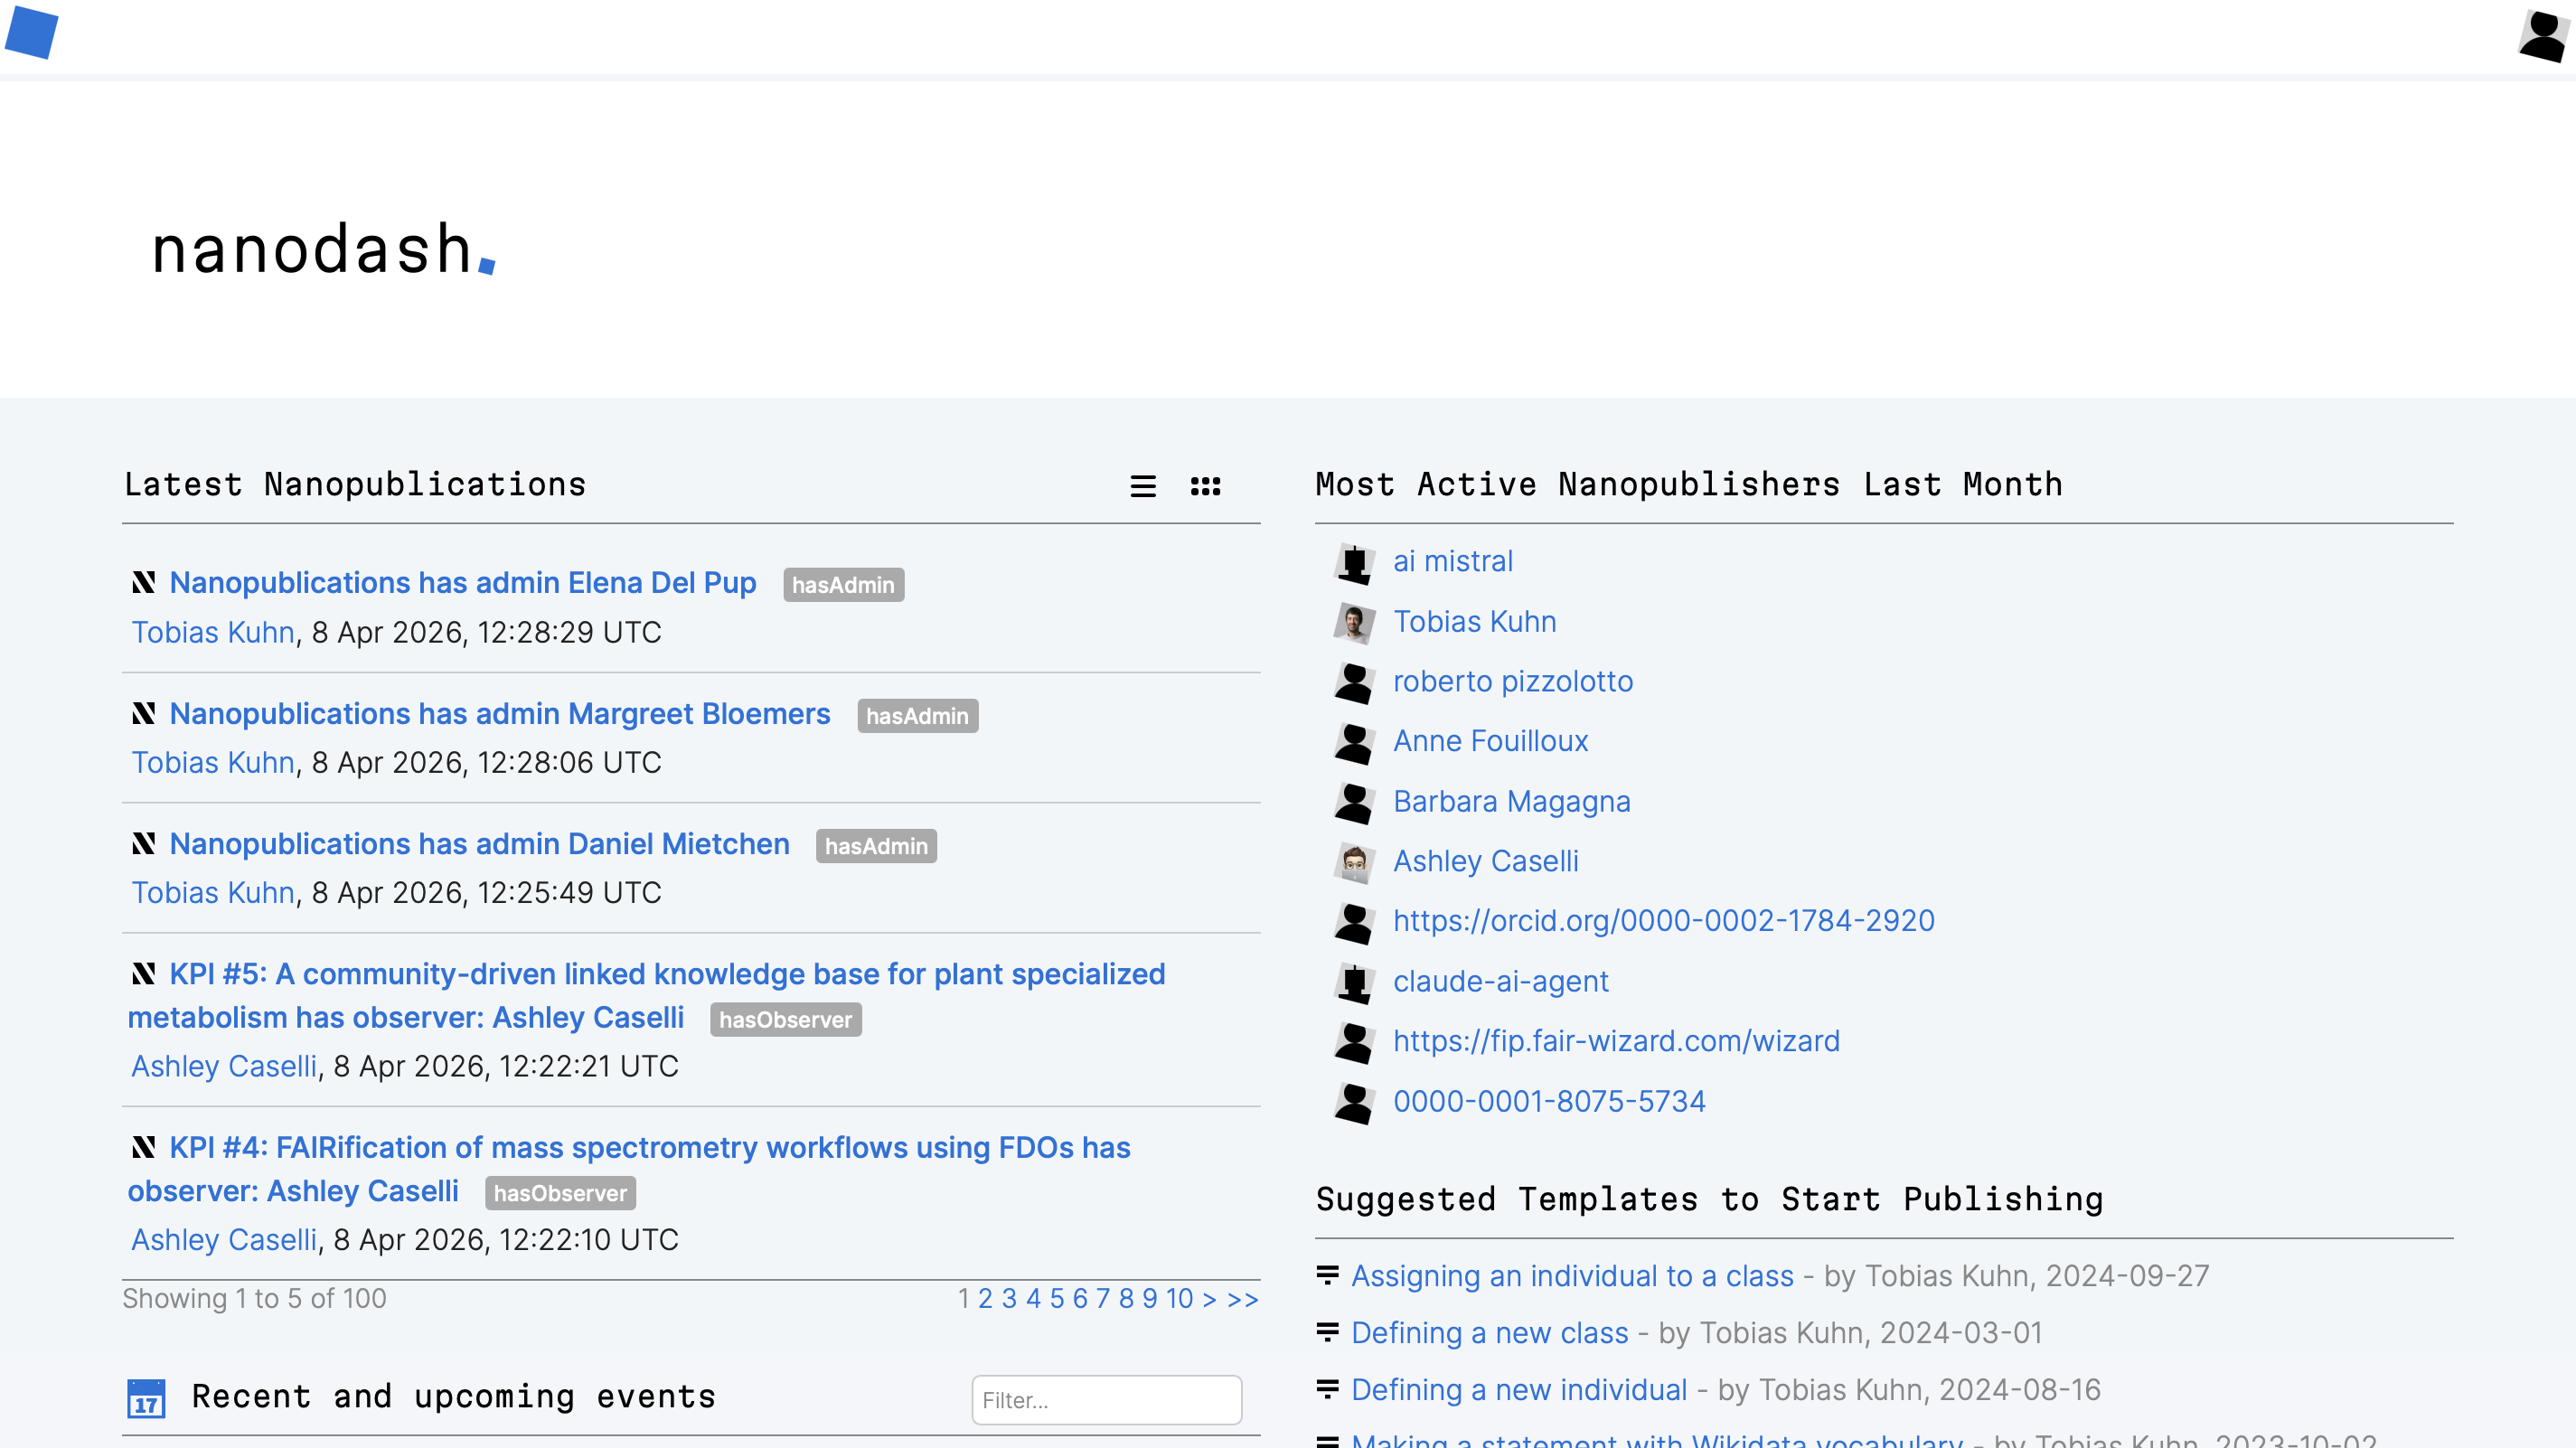
\includegraphics[width=0.9\linewidth]{enter_nanodash.png}
   \end{columns}
}

%%%%%%%%%%%%%%%%%%%%%%%%%%%%%%%%%%%%%%%%%%%%%%%%%%%%%%%%%%%%%%%%%%%%%%%%%%%%%%%%     
\frame{
  \frametitle{Introduction of an User}
  Click on the profile icon in the top right corner to access your profile page.\newline
  \vspace{1em}
  \centering
  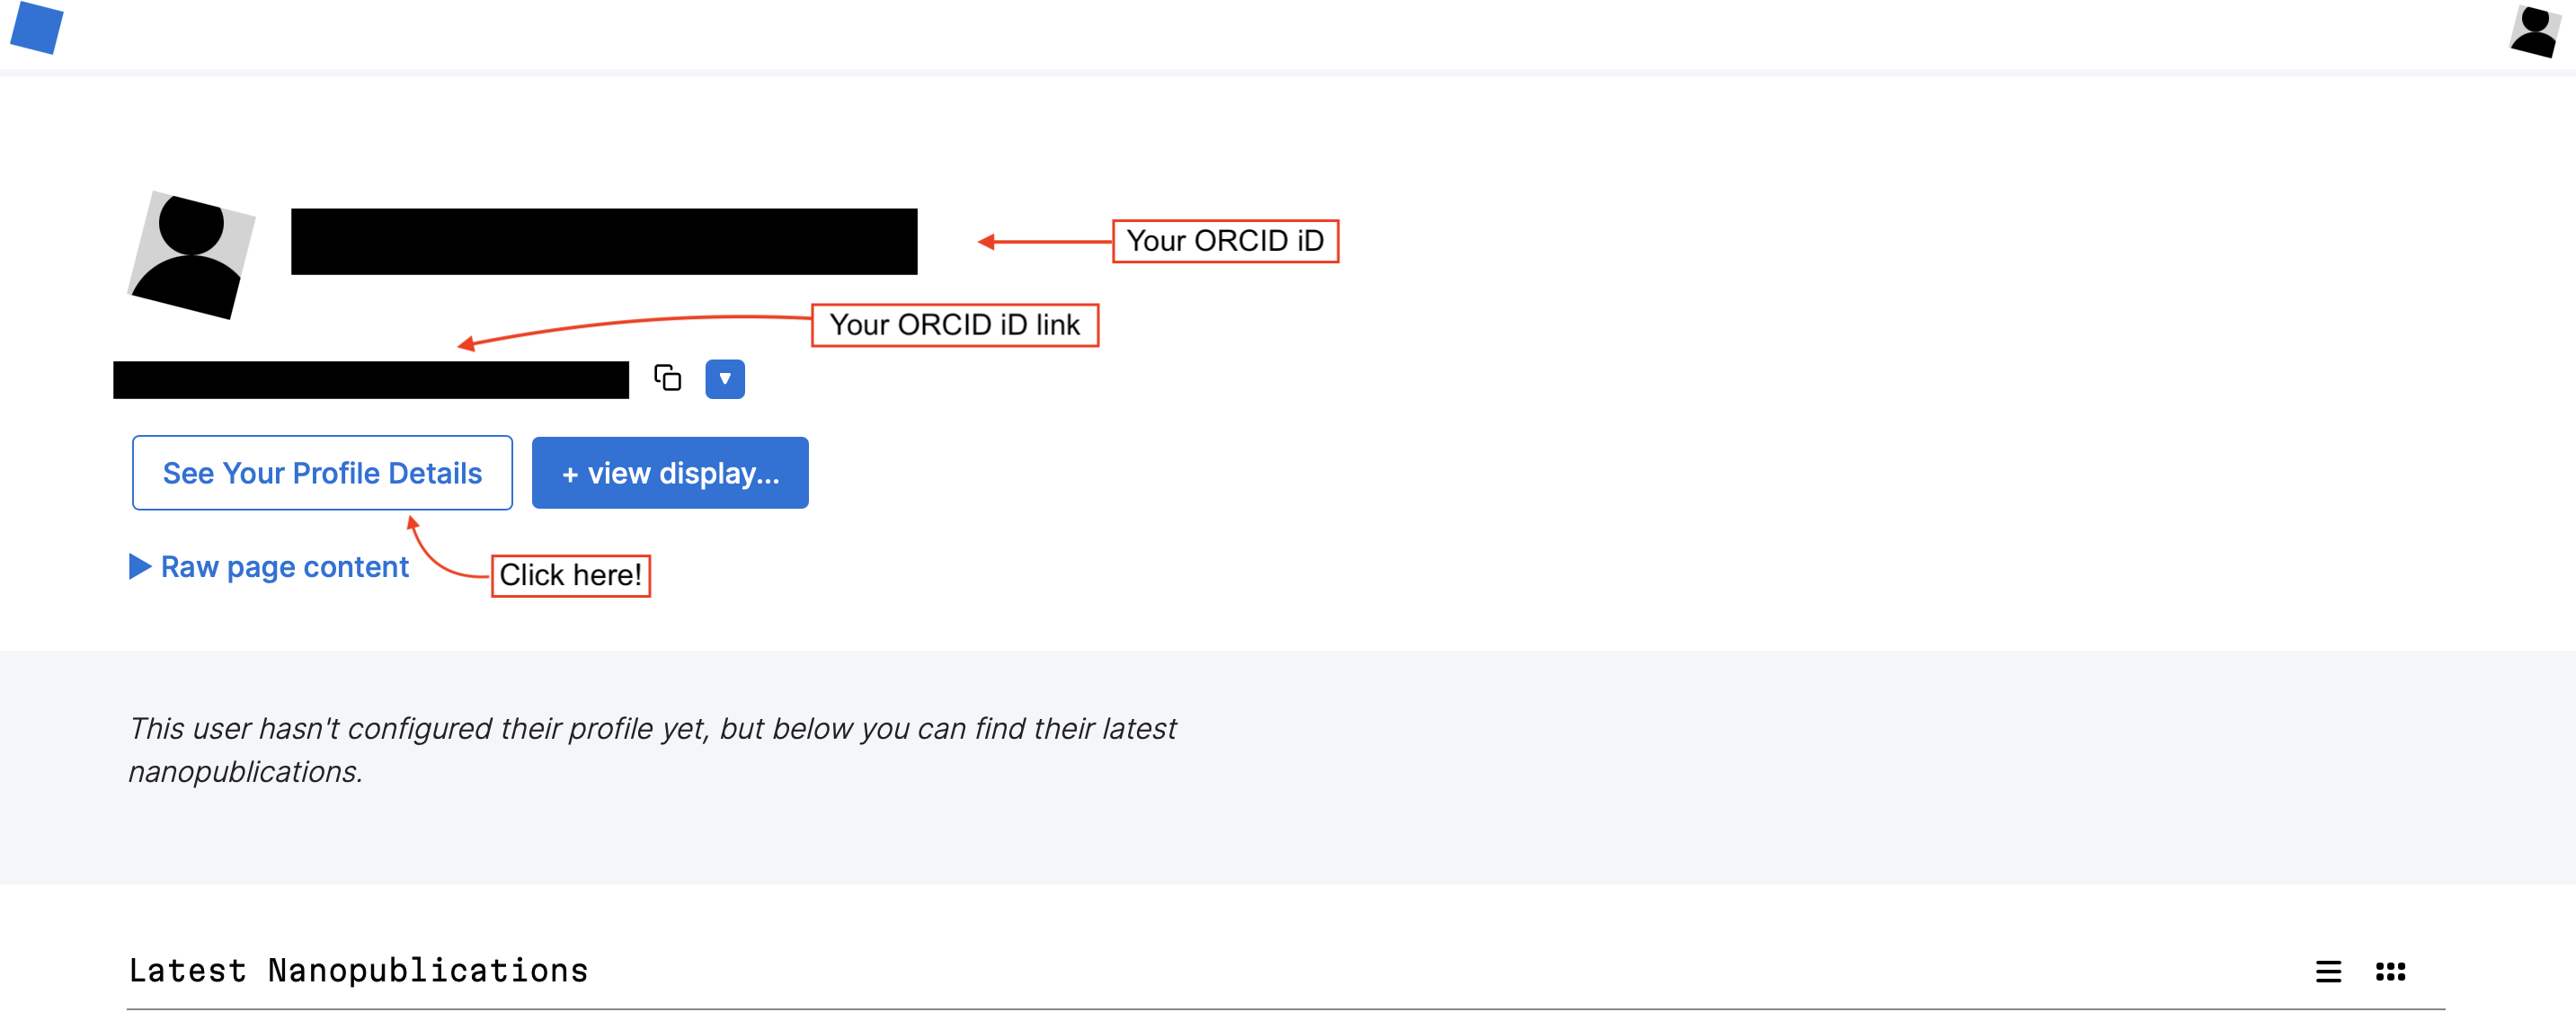
\includegraphics[width=0.8\linewidth]{profile.png} \\
  \vspace{1em}
  Then click on the \textbf{“See Your Profile Details”} button to access your profile details.
}

%%%%%%%%%%%%%%%%%%%%%%%%%%%%%%%%%%%%%%%%%%%%%%%%%%%%%%%%%%%%%%%%%%%%%%%%%%%%%%%%        
\frame{
  \frametitle{Create Introduction}
  Inside the Profile Details page, click on the \textbf{“Create Introduction”} button to create your introduction.
  \vspace{1em}
  \centering
  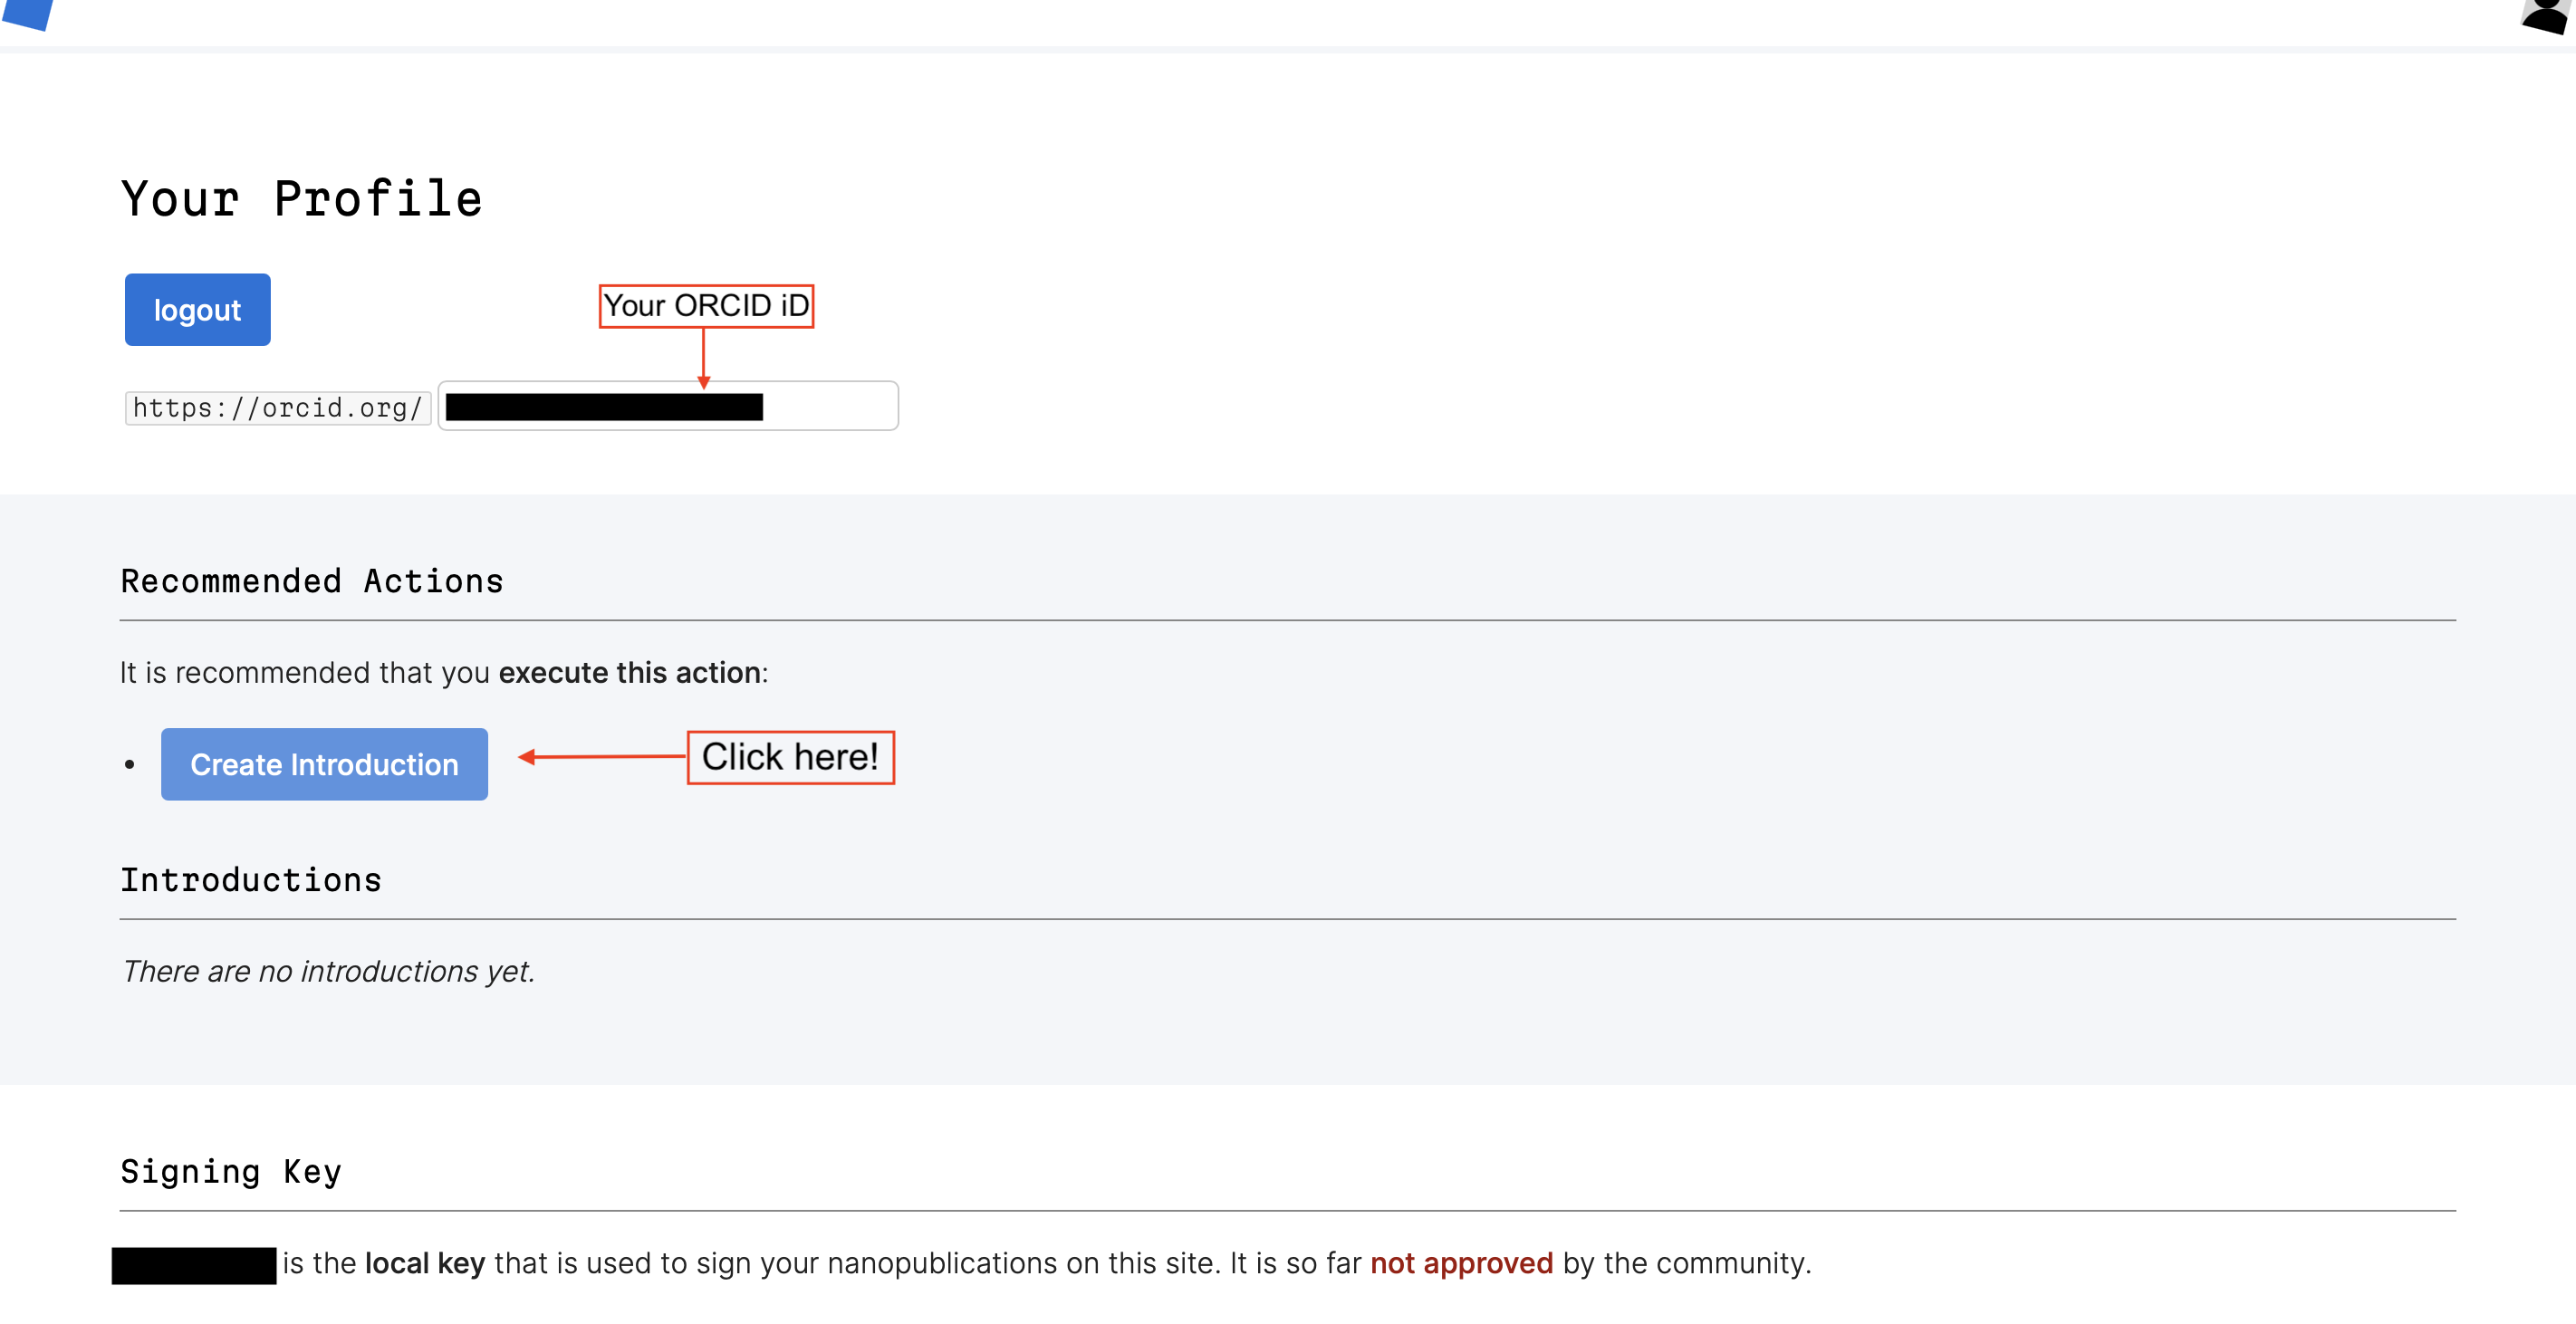
\includegraphics[width=0.8\linewidth]{intro.png}
}
    
%%%%%%%%%%%%%%%%%%%%%%%%%%%%%%%%%%%%%%%%%%%%%%%%%%%%%%%%%%%%%%%%%%%%%%%%%%%%%%%%        
\frame{
  \frametitle{And then ...}
  Once inside the introduction page, you will see a \textbf{“Create Nanopublication”} form.
  \vspace{1em}
  \centering
  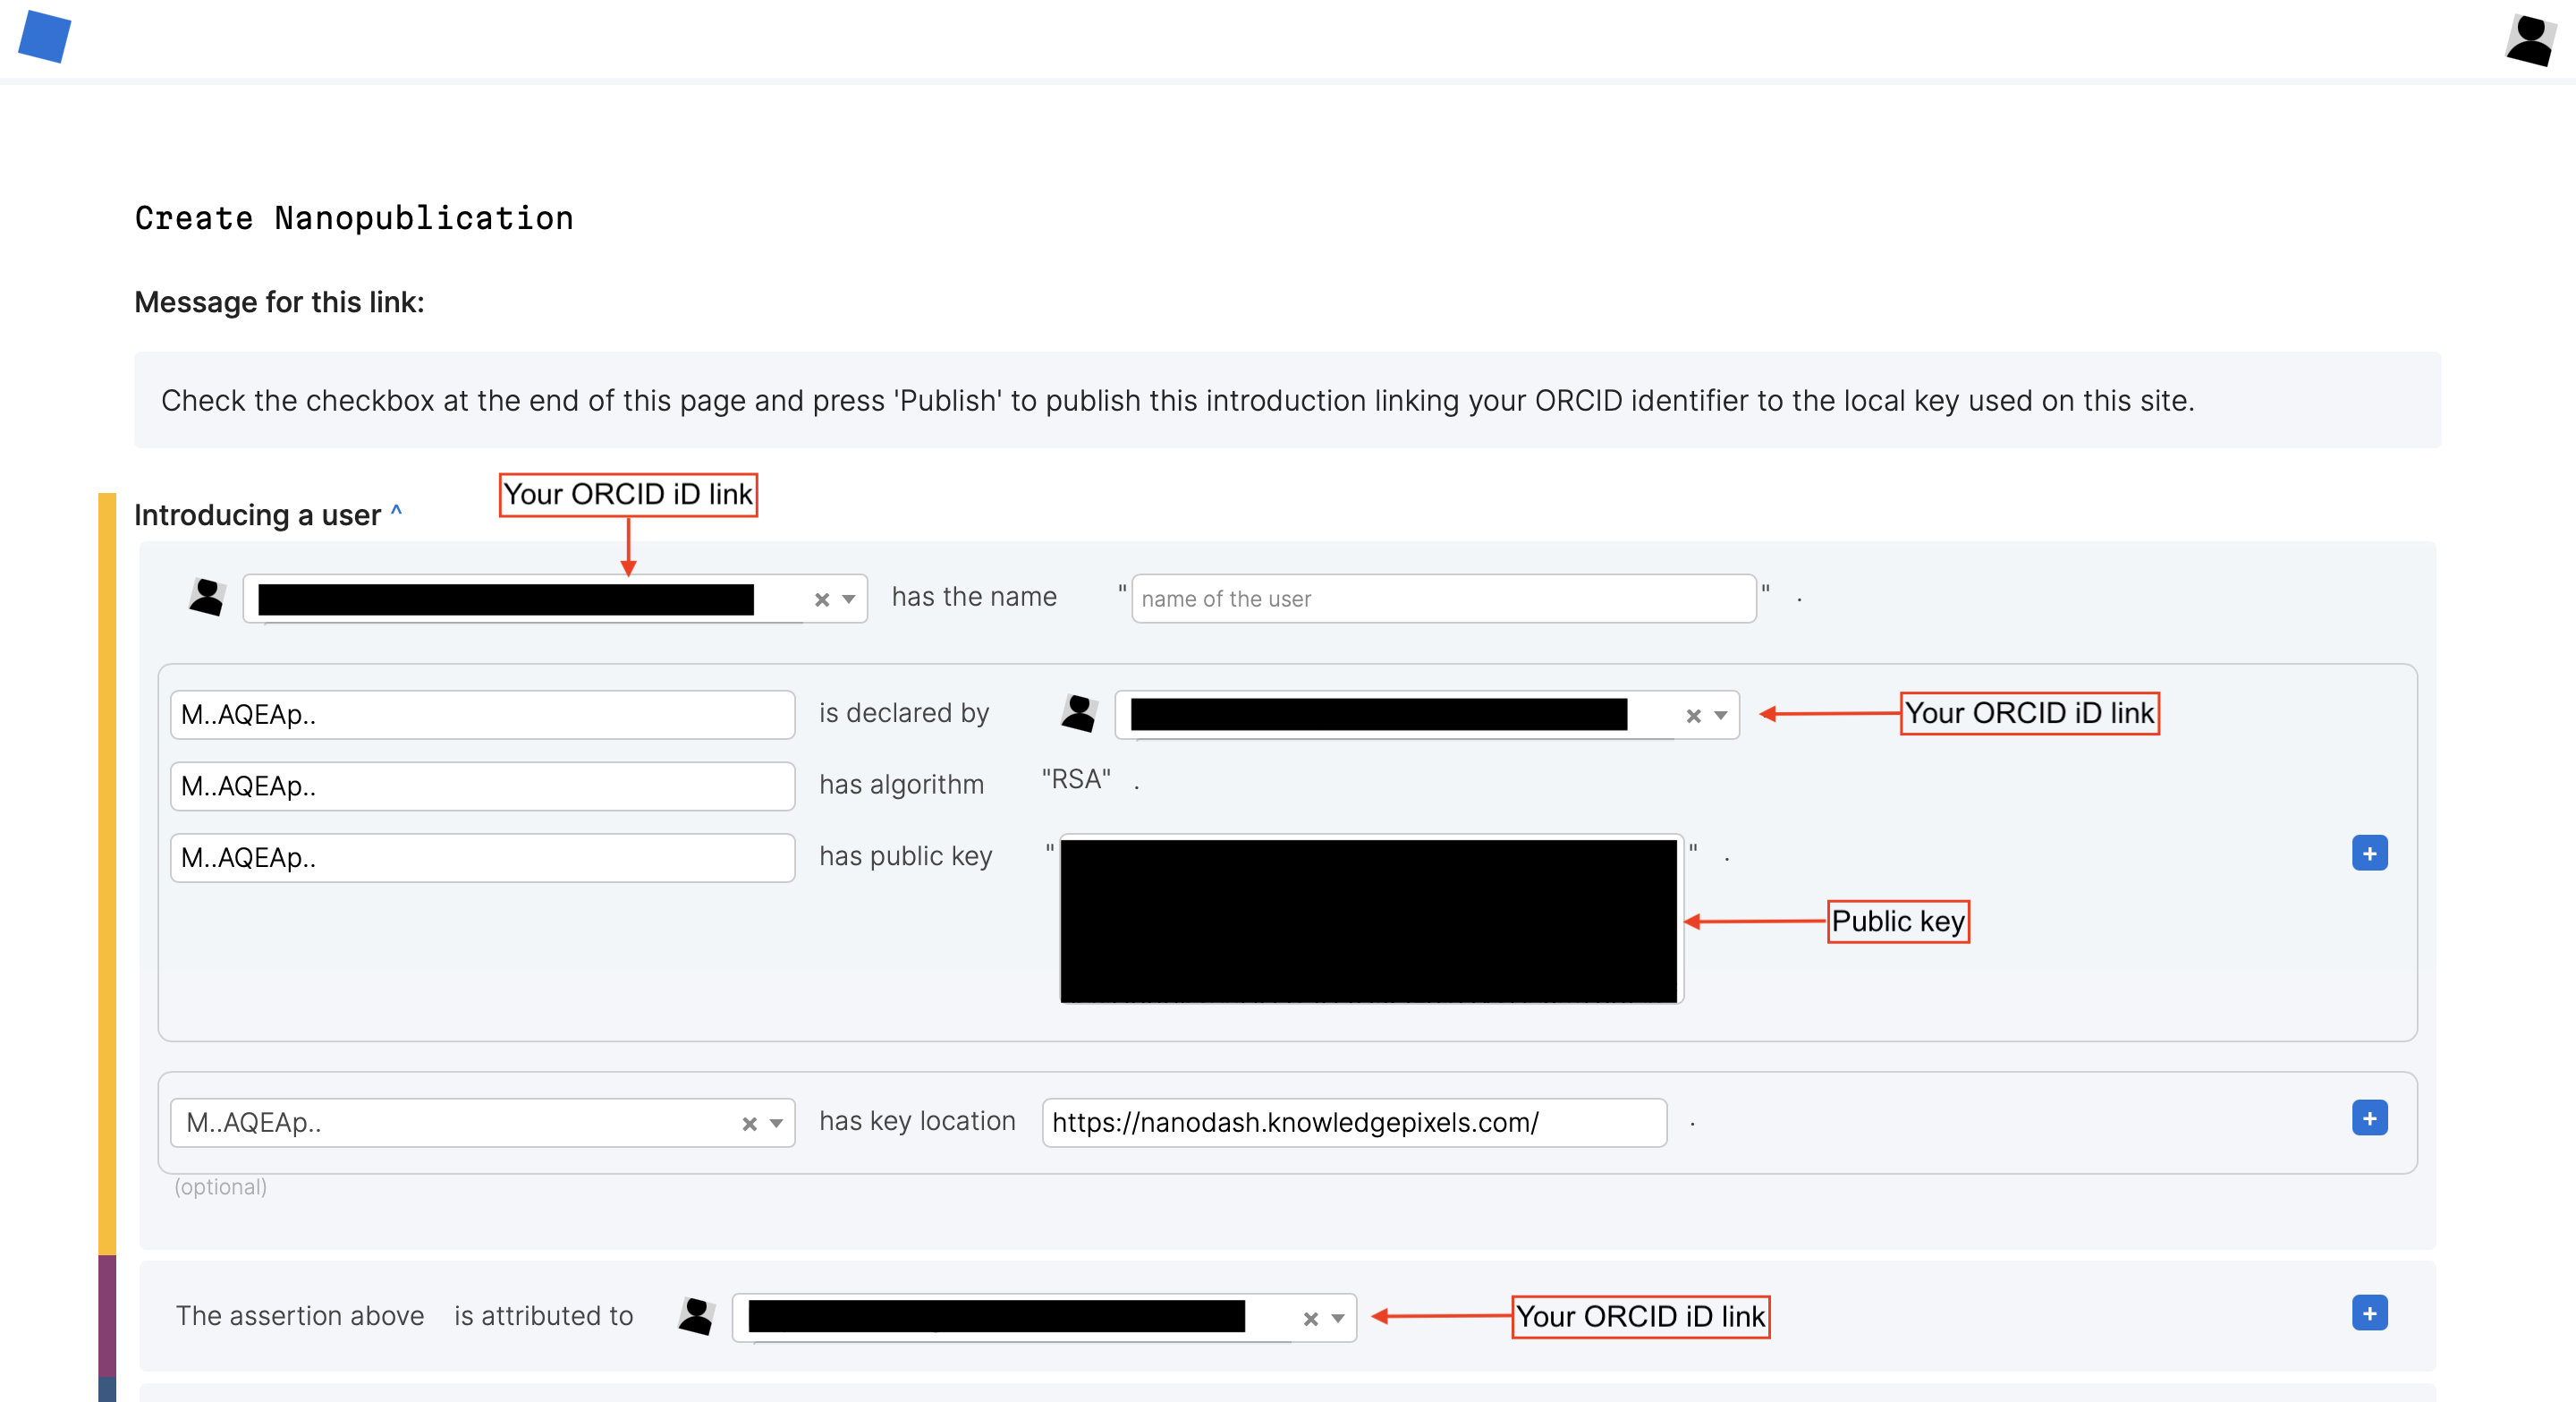
\includegraphics[width=0.8\linewidth]{intro_nanopub.png}
}
    
%%%%%%%%%%%%%%%%%%%%%%%%%%%%%%%%%%%%%%%%%%%%%%%%%%%%%%%%%%%%%%%%%%%%%%%%%%%%%%%%        
\frame{
  \frametitle{Complete your introduction}
  Under the \textbf{“Introducing a user”} section, add your name as you would like it to appear on your profile.
  \vspace{1em}
  \centering
  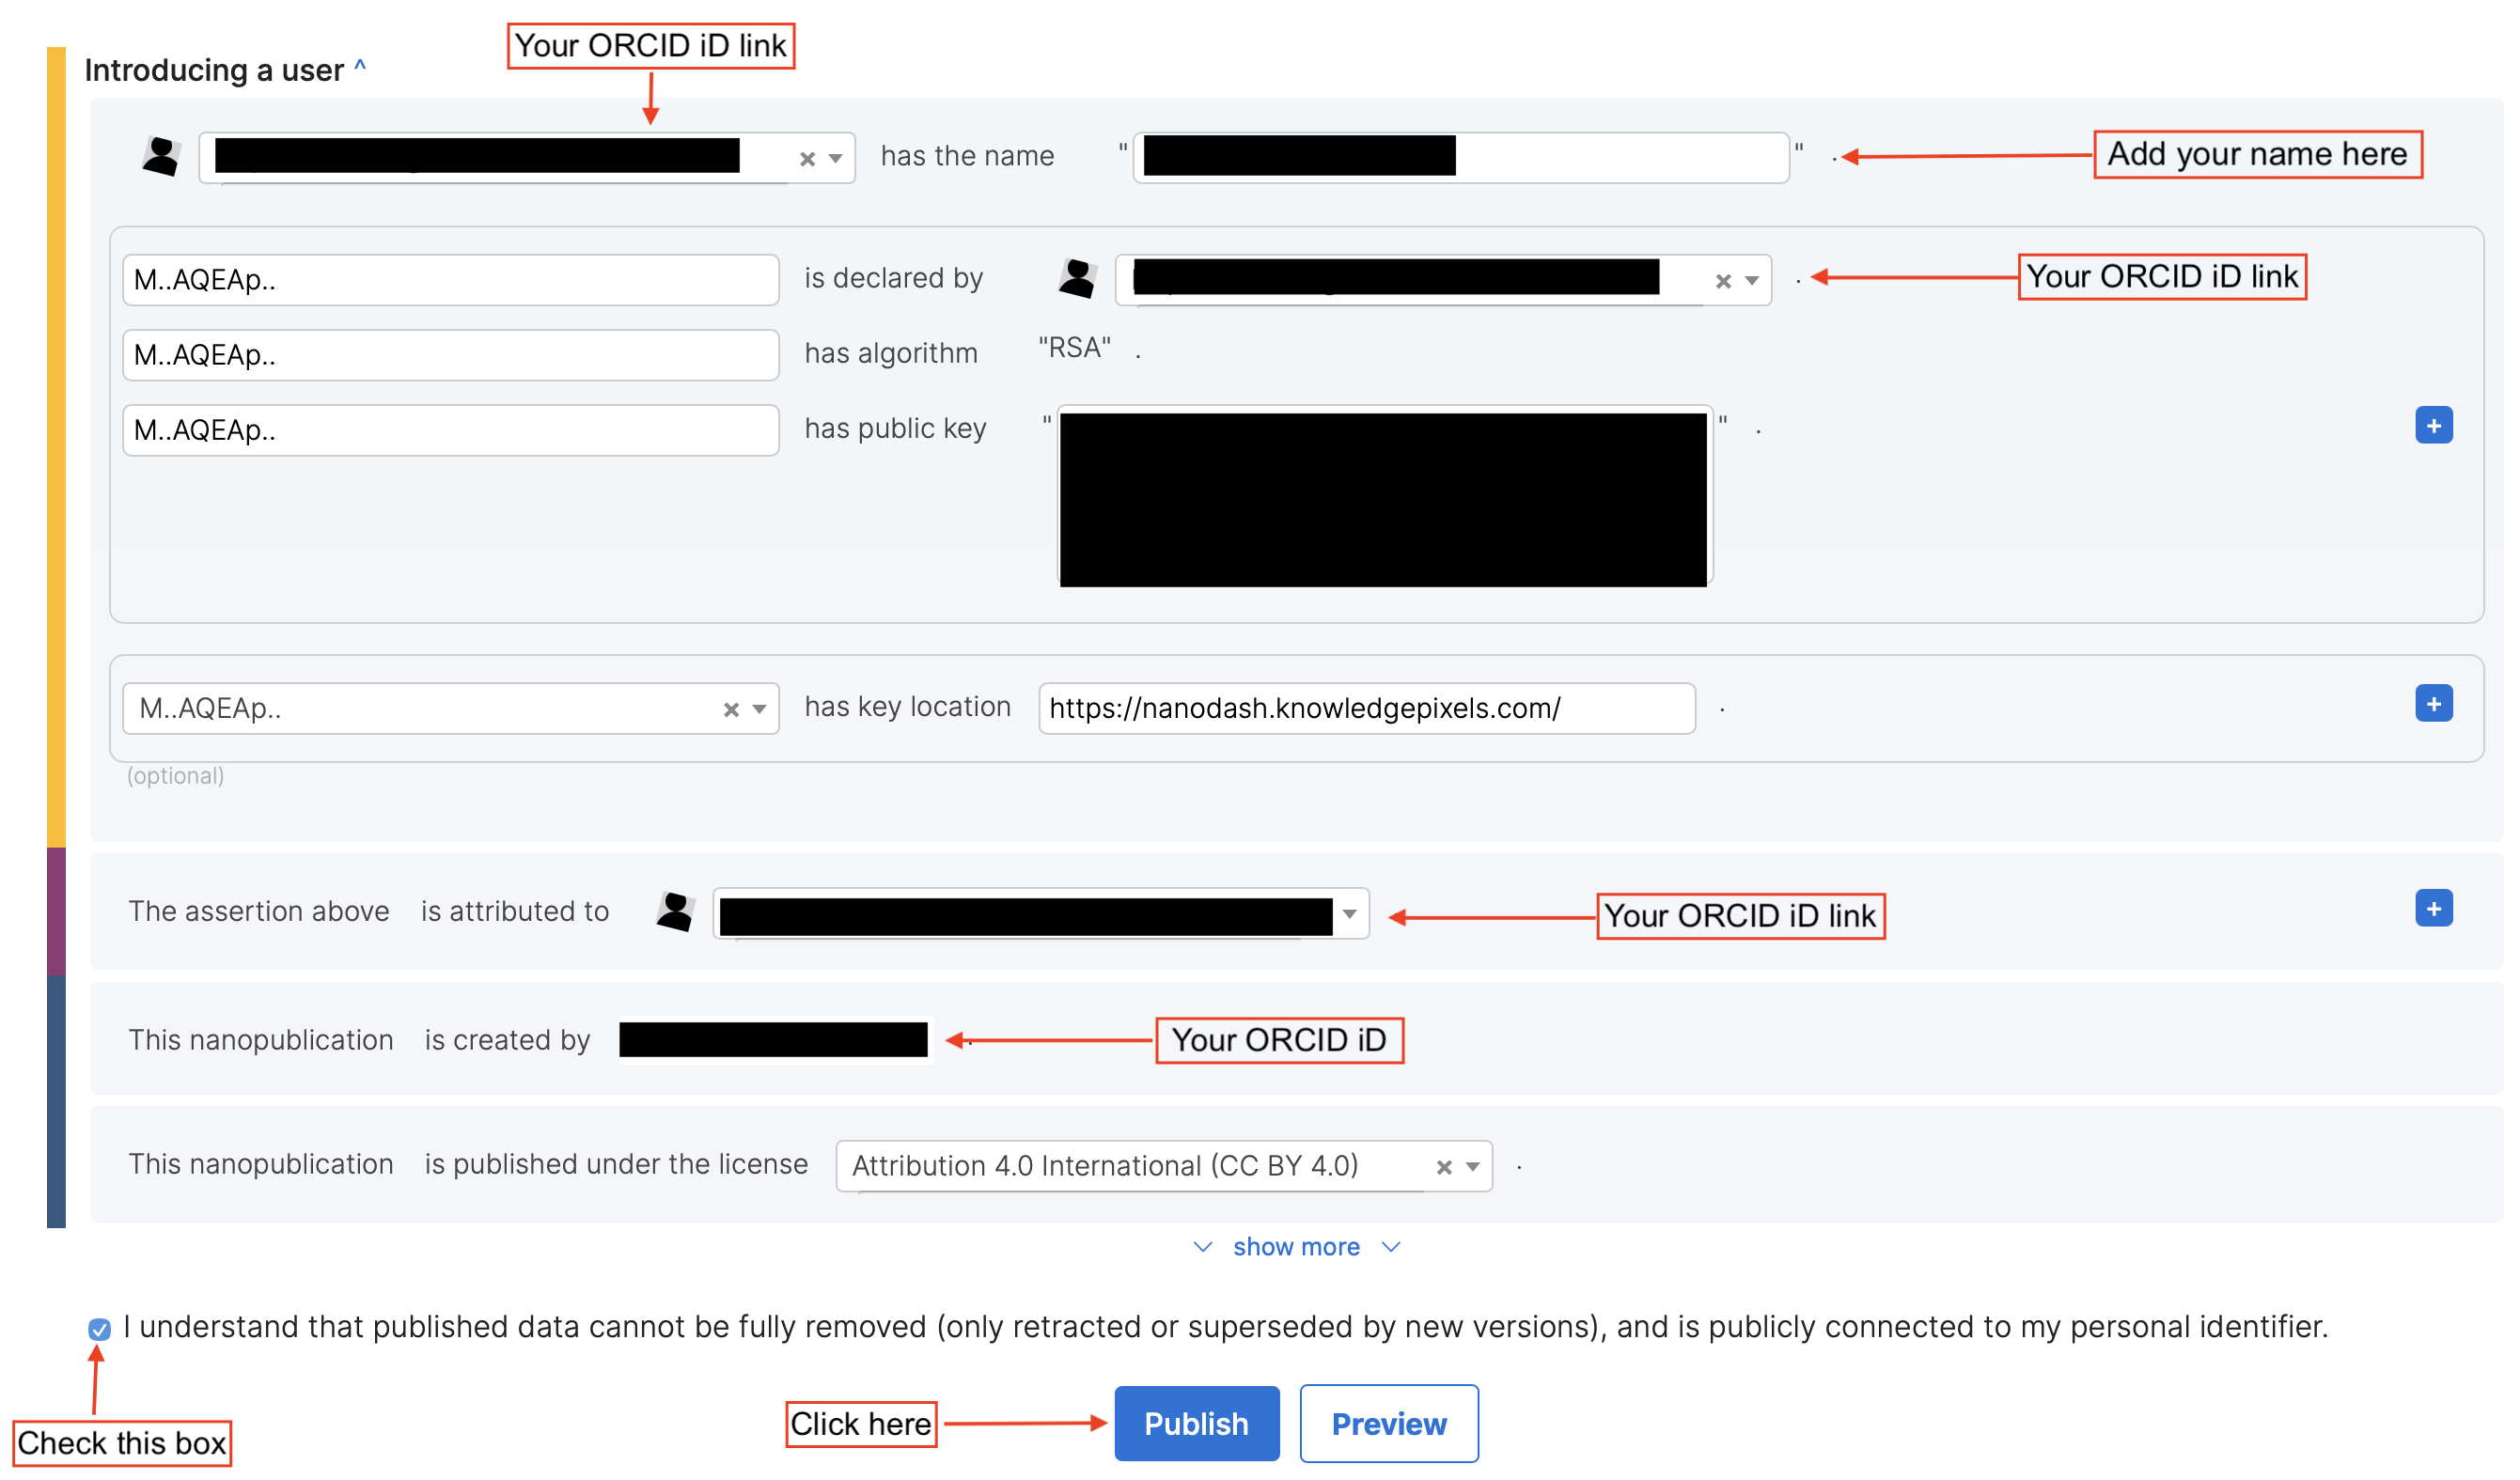
\includegraphics[width=0.8\linewidth]{complete_intro.png} \\
  \vspace{1em}
  Finally, after you are happy, click the \textbf{“Publish”} button to publish your introduction.
}

%%%%%%%%%%%%%%%%%%%%%%%%%%%%%%%%%%%%%%%%%%%%%%%%%%%%%%%%%%%%%%%%%%%%%%%%%%%%%%%%    
\frame{
  \frametitle{A published introduction ...}
  Once the introduction is published, you should now be able to view your name on it.
  \vspace{1em}
  \centering
  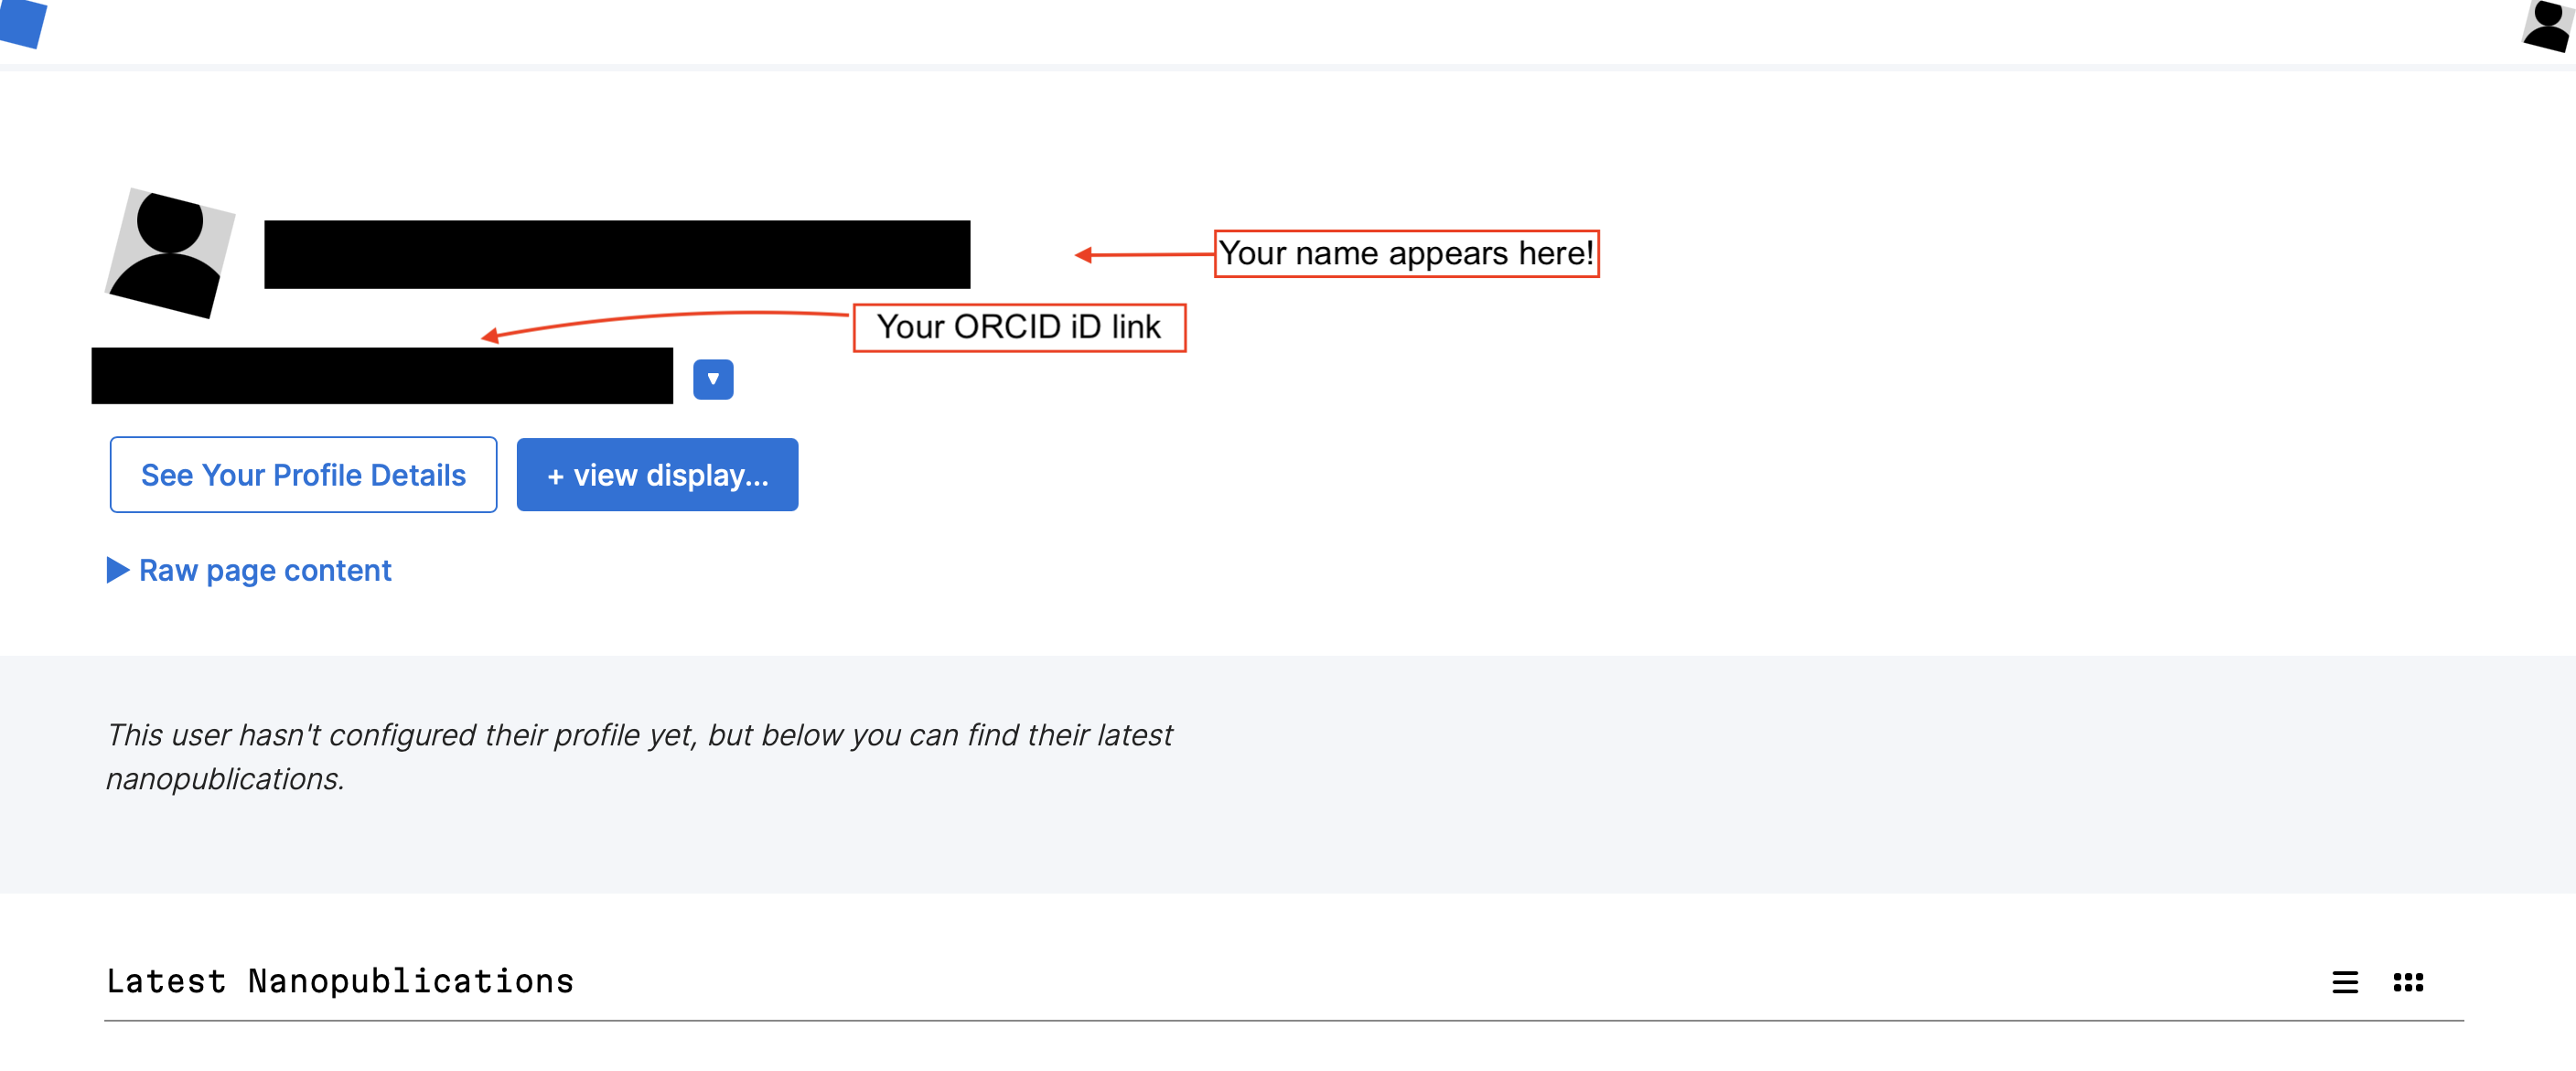
\includegraphics[width=0.8\linewidth]{name_profile.png}
}

%%%%%%%%%%%%%%%%%%%%%%%%%%%%%%%%%%%%%%%%%%%%%%%%%%%%%%%%%%%%%%%%%%%%%%%%%%%%%%%% 
\frame{
  \frametitle{View the latest Nanopubs}
  Your name will appear under the latest nanopublications on your profile page.
  \vspace{1em}
  \centering
  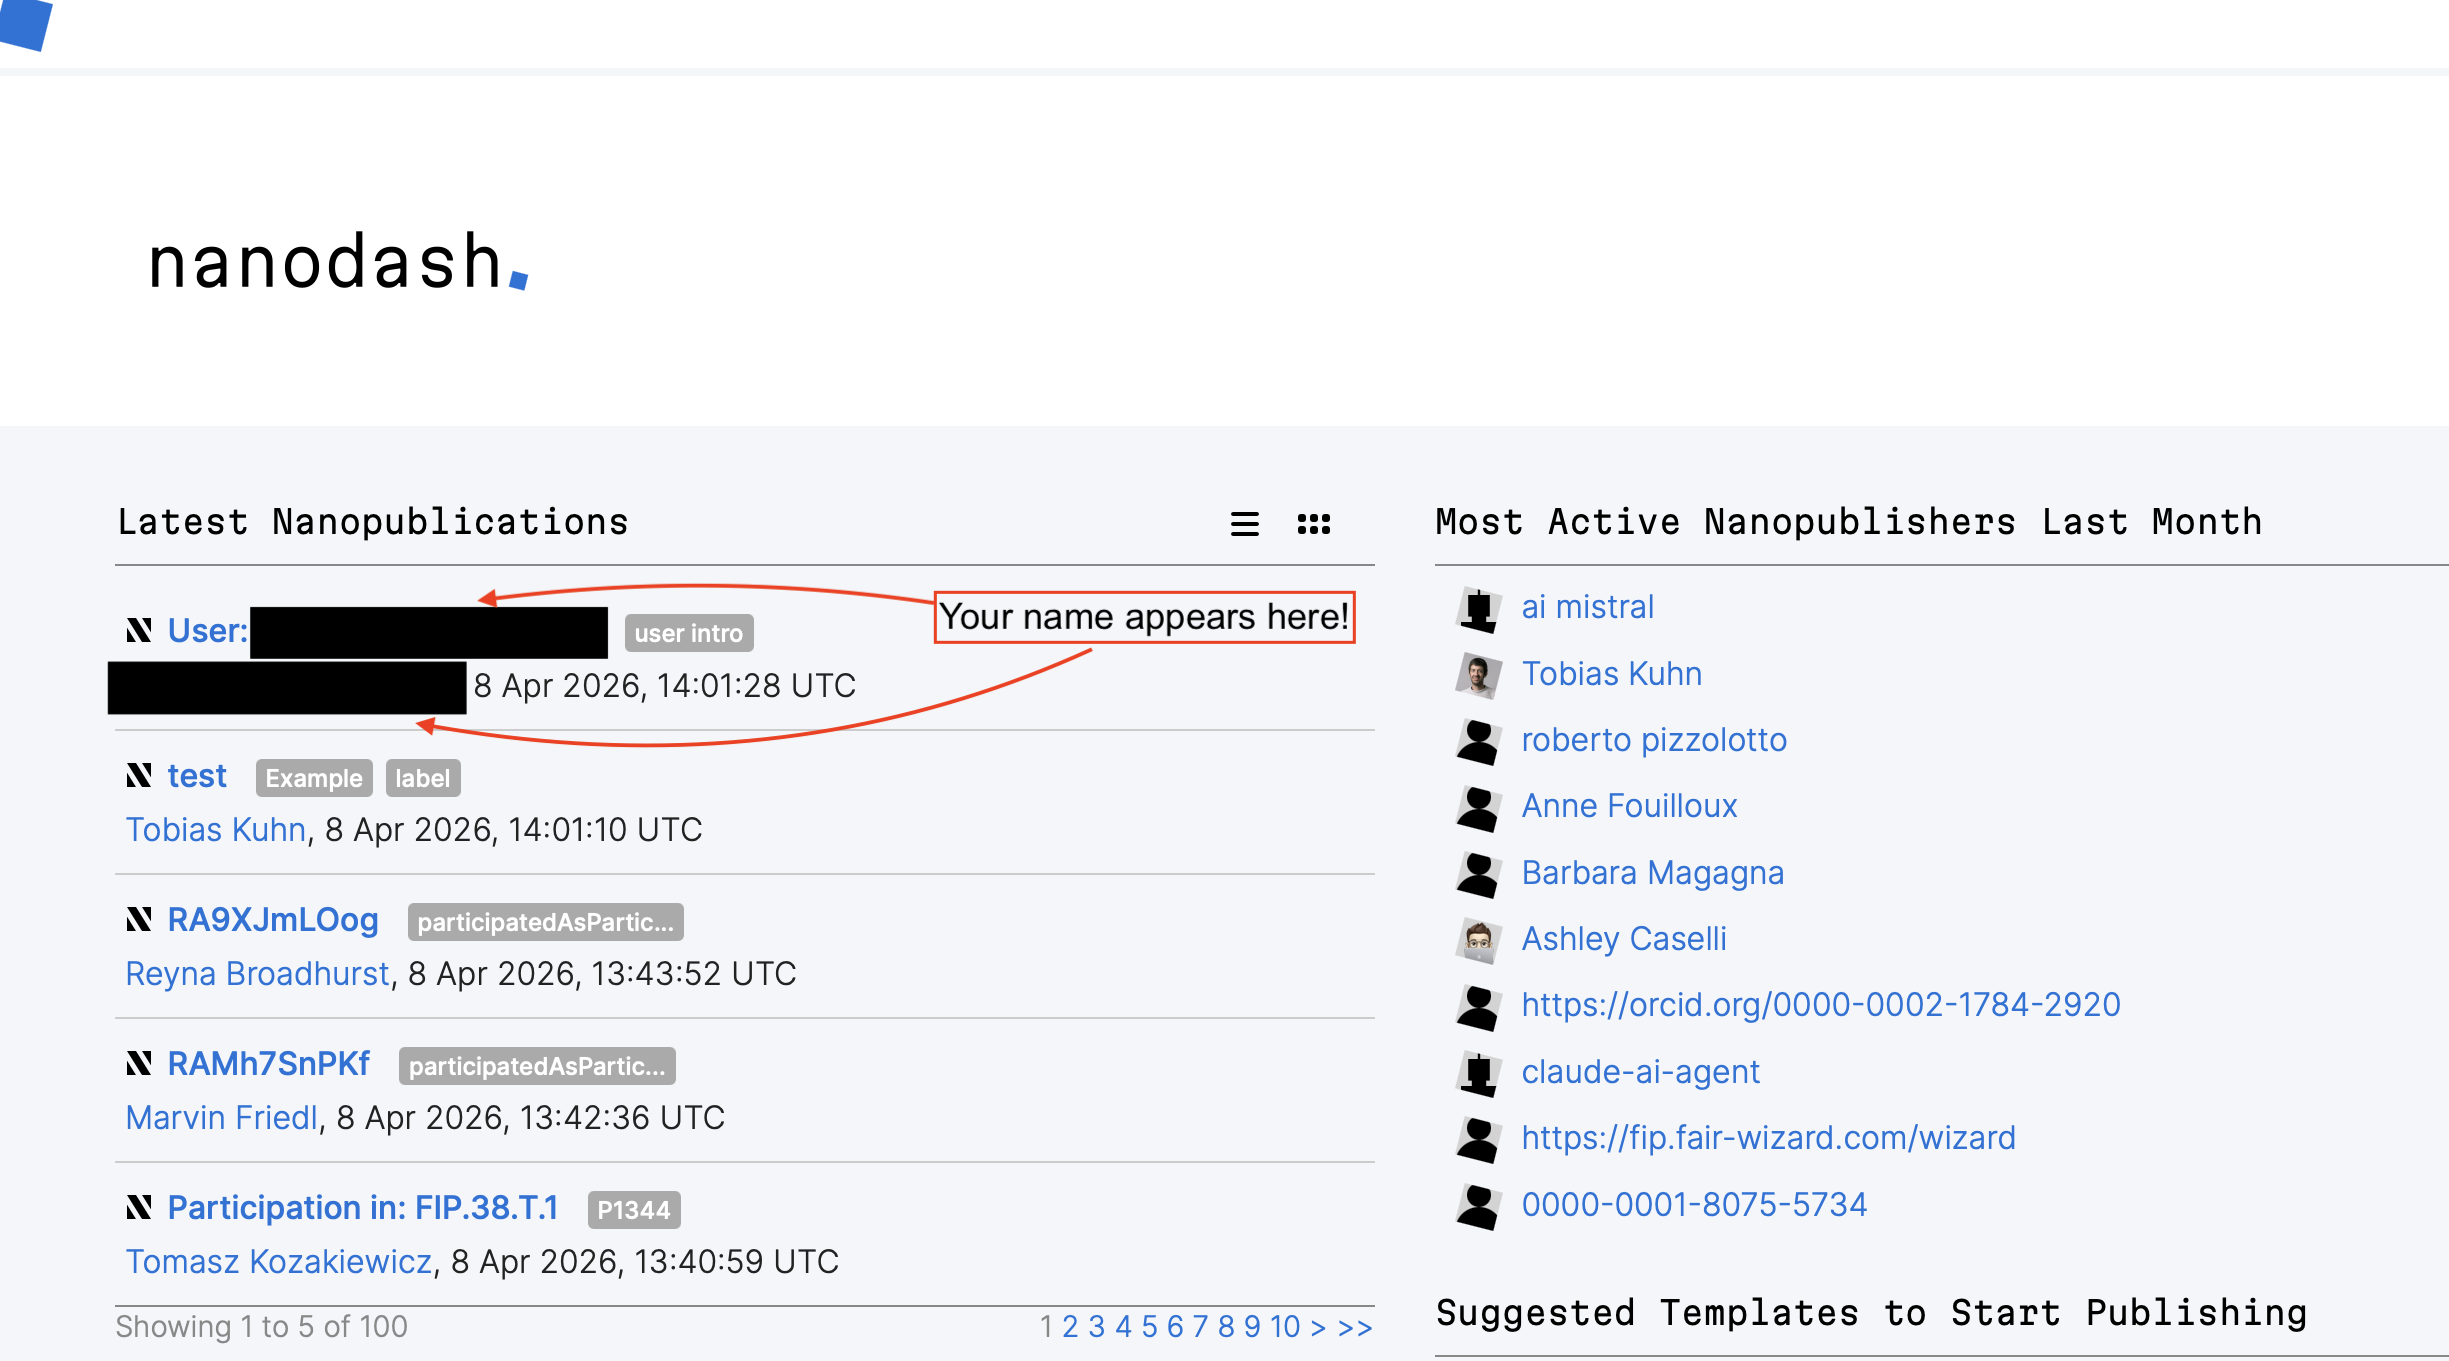
\includegraphics[width=0.8\linewidth]{latest_nano.png}
}

%%%%%%%%%%%%%%%%%%%%%%%%%%%%%%%%%%%%%%%%%%%%%%%%%%%%%%%%%%%%%%%%%%%%%%%%%%%%%%%%    
\frame{
  \frametitle{Add “view display” to your profile}
  To add display sections to your profile, click on the \textbf{“+ view display”} button; a new page for adding a display section will open.
  \begin{columns}[T]
     \column{0.5\textwidth}
     \centering
     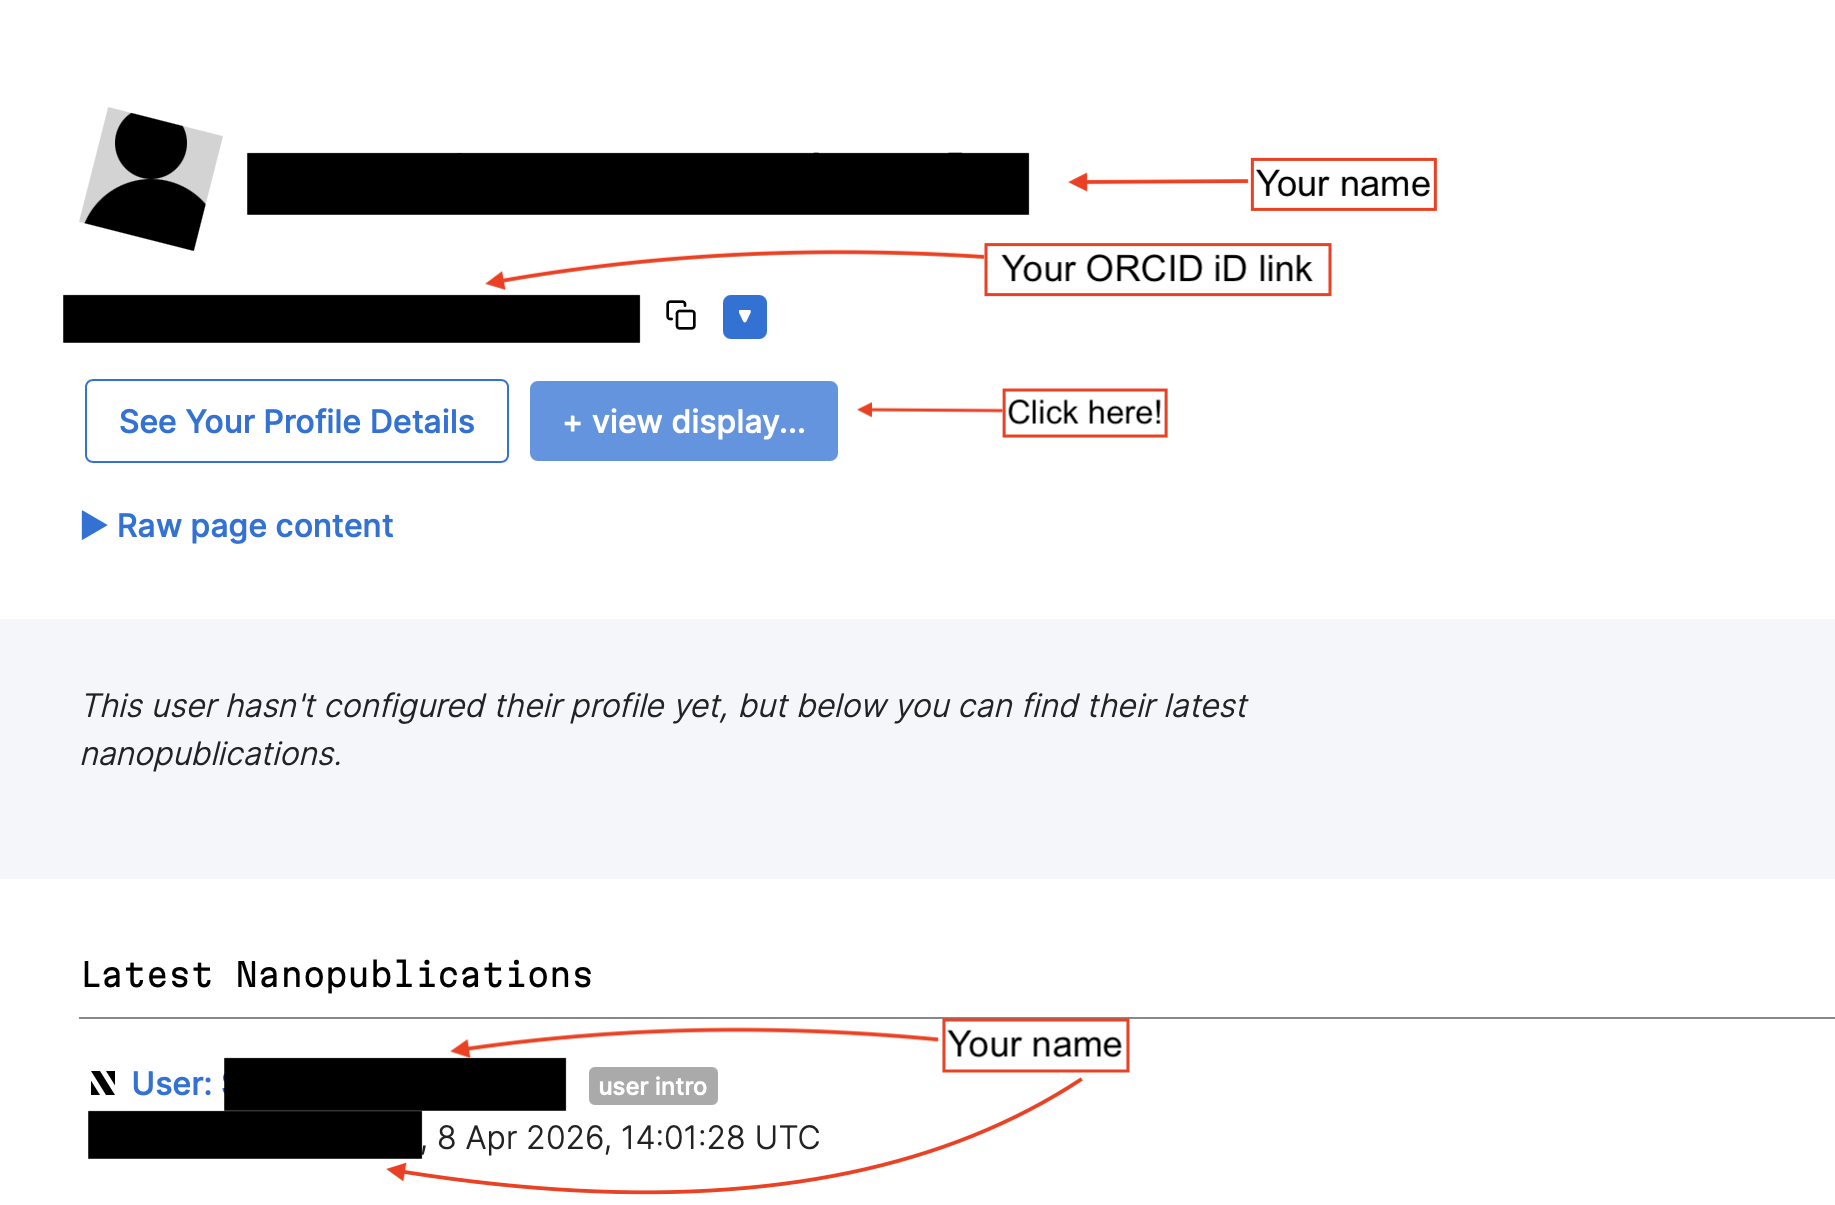
\includegraphics[width=0.9\linewidth]{view_display.png}
     \column{0.5\textwidth}
     \centering
     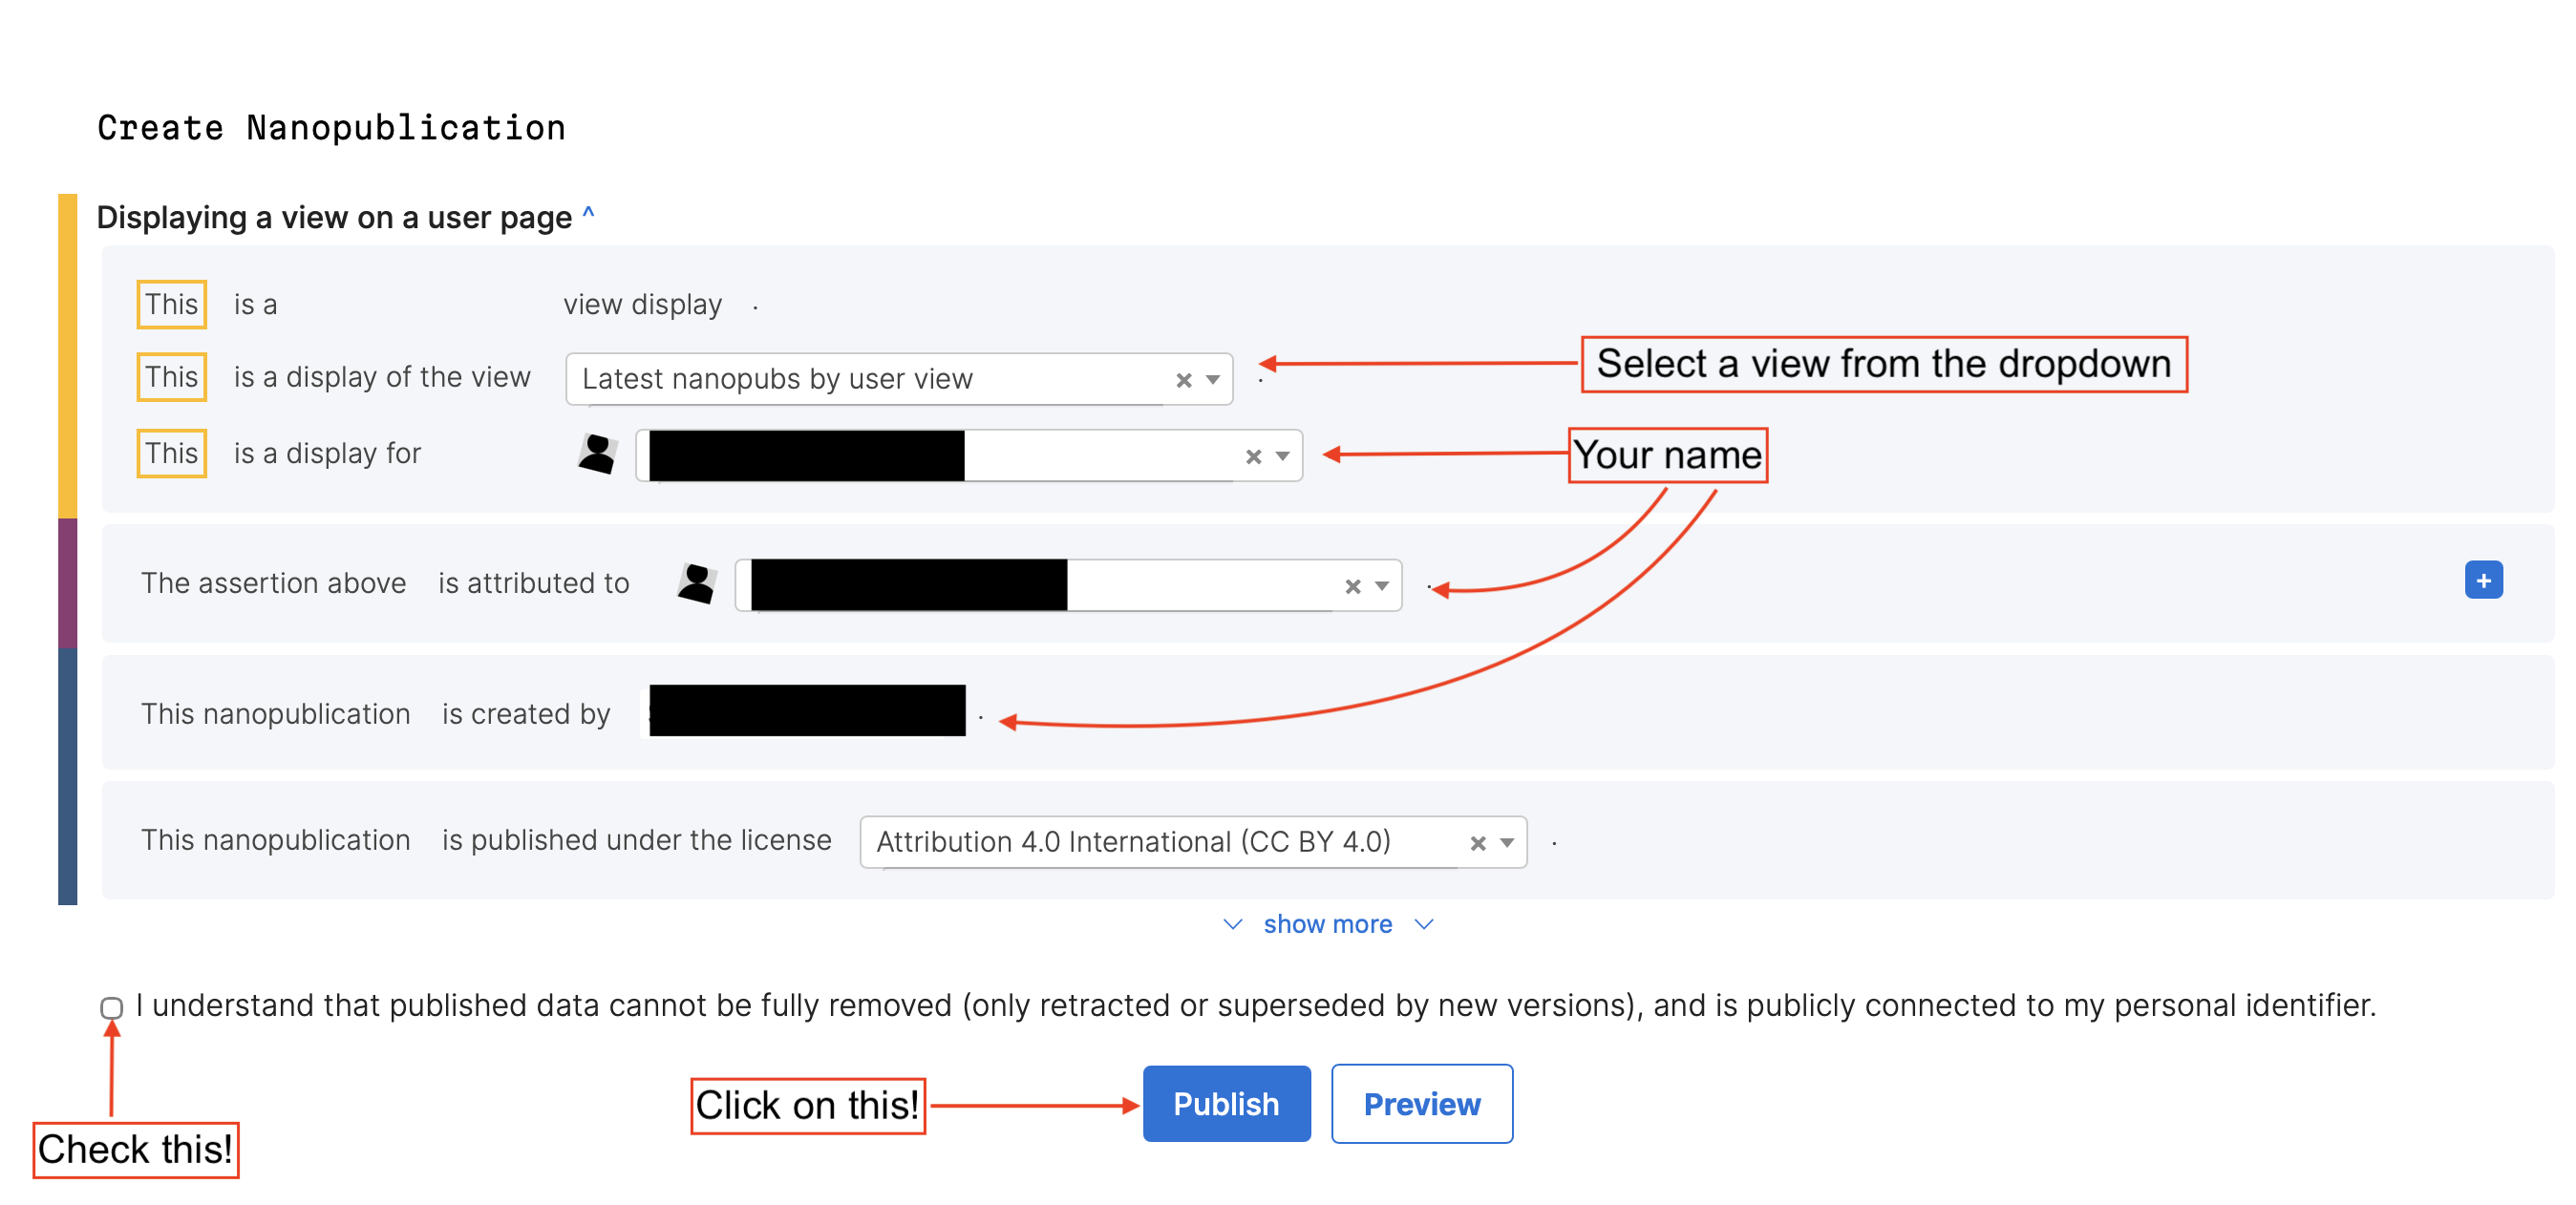
\includegraphics[width=0.9\linewidth]{create_view_display.png}
  \end{columns}
}
    
%%%%%%%%%%%%%%%%%%%%%%%%%%%%%%%%%%%%%%%%%%%%%%%%%%%%%%%%%%%%%%%%%%%%%%%%%%%%%%%%    
\frame{
  \frametitle{Approval of an User}
  Next on our list: approval of a user. Users can be approved by approved users.
  \vspace{1em}
  \centering
  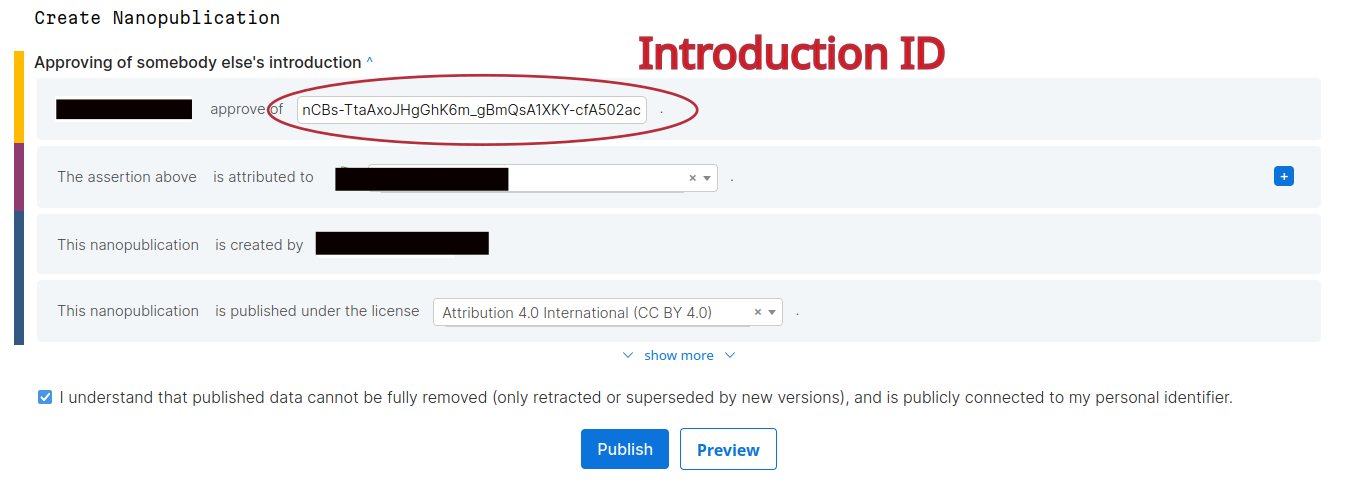
\includegraphics[width=0.8\linewidth]{approval_with_highlighting.png} \\
  \vspace{1em}
  \textbf{Task:} approve your neighbour(s)!
}
    
%%%%%%%%%%%%%%%%%%%%%%%%%%%%%%%%%%%%%%%%%%%%%%%%%%%%%%%%%%%%%%%%%%%%%%%%%%%%%%%%    
\frame{
  \frametitle{Publish from a Template}
  \begin{columns}[T]
            \column{0.3\textwidth}
            \centering
            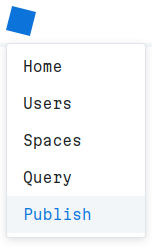
\includegraphics[width=\linewidth]{publish_menu.png} \\
            Select \textbf{“Publish”} from the menu.
            \column{0.7\textwidth}
            \centering
            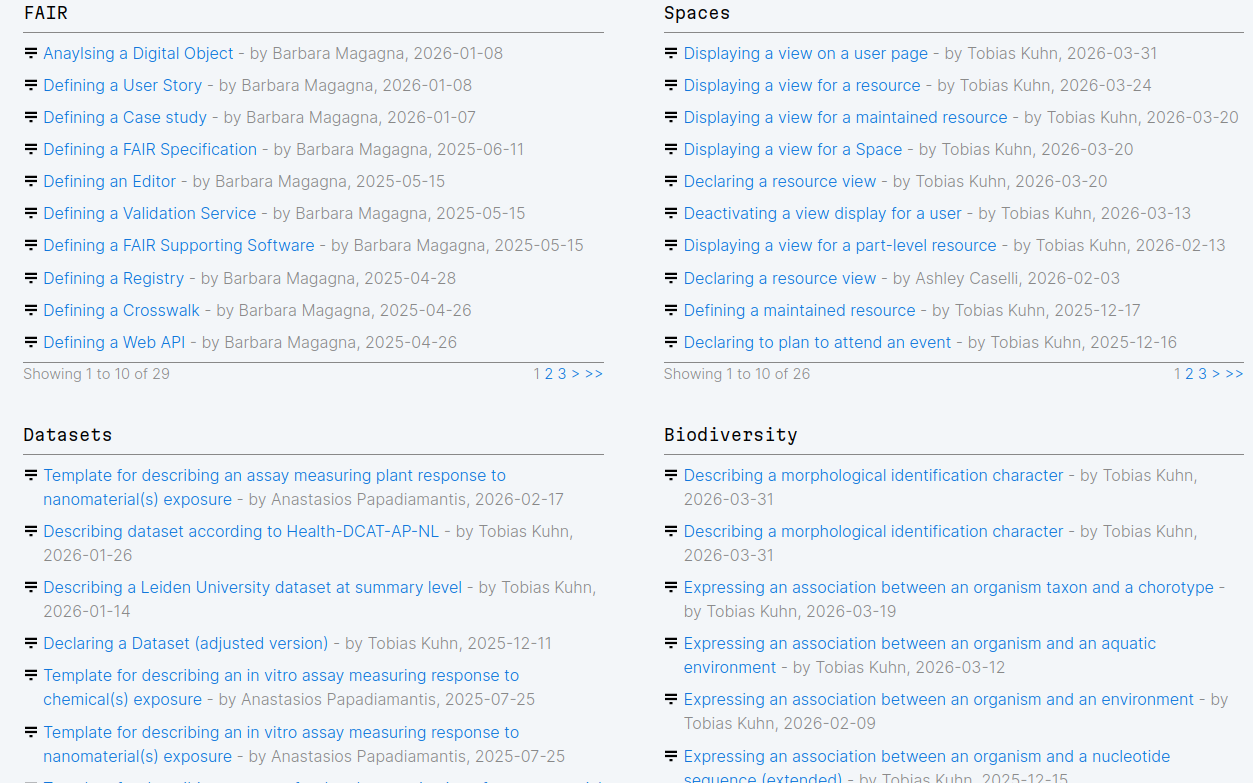
\includegraphics[width=\linewidth]{publish_templates.png} \\
            Then you \textbf{can} choose from the list of templates. (We are going to publish together. Please wait.)
        \end{columns}
}

%%%%%%%%%%%%%%%%%%%%%%%%%%%%%%%%%%%%%%%%%%%%%%%%%%%%%%%%%%%%%%%%%%%%%%%%%%%%%%%%    
    \frame{
        \frametitle{Your first Nanopub!}
        Let’s select an easy template: search for \textbf{“Announcing a paper I have read”}.
        \vspace{1em}
        \centering
        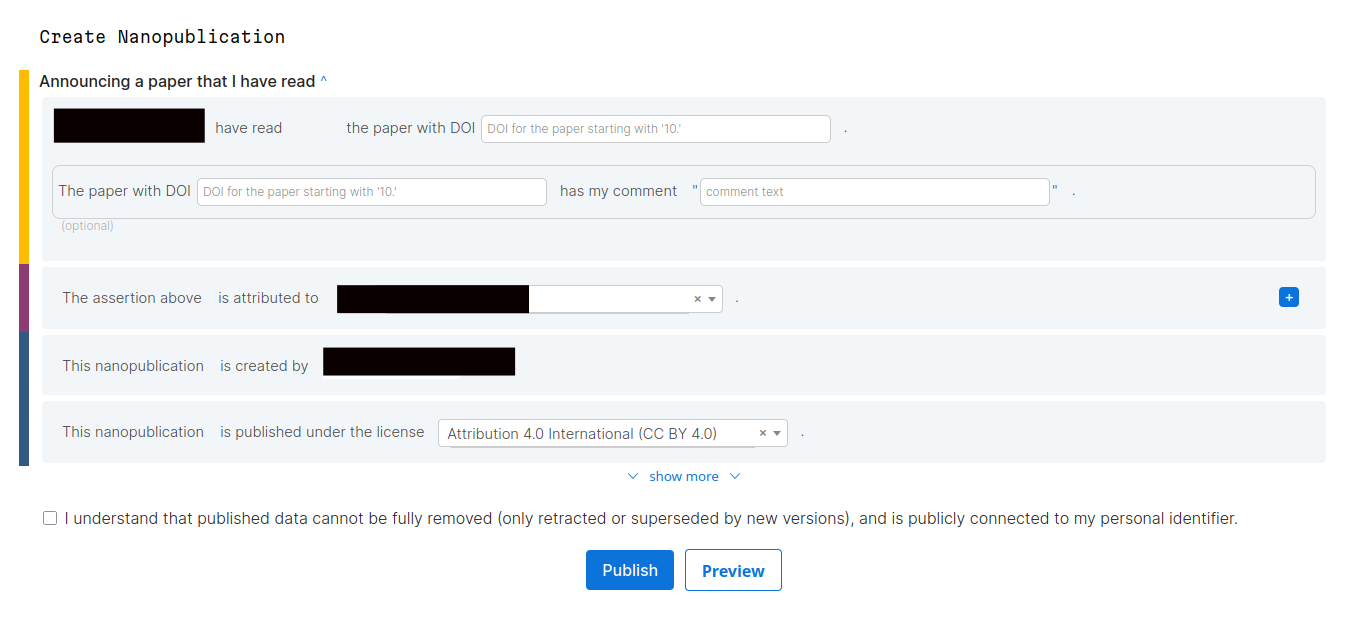
\includegraphics[width=0.8\linewidth]{publish_paper_read.png} \\
        \vspace{1em}
        Select the template and enter the DOI of a recently read paper.
    }

%%%%%%%%%%%%%%%%%%%%%%%%%%%%%%%%%%%%%%%%%%%%%%%%%%%%%%%%%%%%%%%%%%%%%%%%%%%%%%%%    
    \frame{
        \frametitle{Modifying a Template}
        There are many templates for different purposes and disciplines. \textit{But}, sometimes you need a new template \dots
        \vspace{1em}
        \begin{callouttip}
            \textbf{First look, then leap} \\
            It is better not to “pollute” the nanopub template space. First look or ask for existing templates.
        \end{callouttip}
        \vspace{1em}
        \begin{calloutnote}
            We are \textbf{not} going to create a new template in this workshop, but we will briefly show you how it’s done.
        \end{calloutnote}
    }
    
%%%%%%%%%%%%%%%%%%%%%%%%%%%%%%%%%%%%%%%%%%%%%%%%%%%%%%%%%%%%%%%%%%%%%%%%%%%%%%%%  
    \frame{
        \frametitle{Modifying a Template II}
        \begin{itemize}
            \item<+-> Start by selecting a suitable (similar) template and click the little blue caret \\
            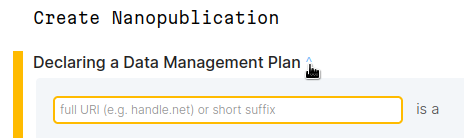
\includegraphics[width=0.4\linewidth]{new_template_01.png}
            \item<+-> Then select \textbf{“edit as derived nanopublication”} \\
            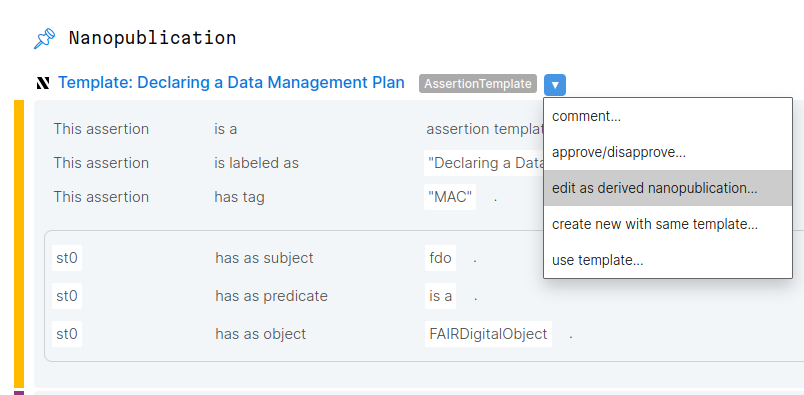
\includegraphics[width=0.6\linewidth]{new_template_02.png}
        \end{itemize}
    }

%%%%%%%%%%%%%%%%%%%%%%%%%%%%%%%%%%%%%%%%%%%%%%%%%%%%%%%%%%%%%%%%%%%%%%%%%%%%%%%%    
    \frame{
        \frametitle{Modifying a Template III}
        \begin{callouttip}
            \textbf{Start small} \\
            Creating a new assertion template can be difficult. Start with an easy (or small) one.
        \end{callouttip}
        \vspace{1em}
        \begin{callouttip}
            \textbf{Ask for input!} \\
            If you need substantial changes, ask for help. (In the end we will show some resources.)
        \end{callouttip}
    }

%%%%%%%%%%%%%%%%%%%%%%%%%%%%%%%%%%%%%%%%%%%%%%%%%%%%%%%%%%%%%%%%%%%%%%%%%%%%%%%%
    \frame{
        \frametitle{What can you do with Nanopubs?}
        Construct knowledge-graphs for your paper!
        \vspace{1em}
        \centering
        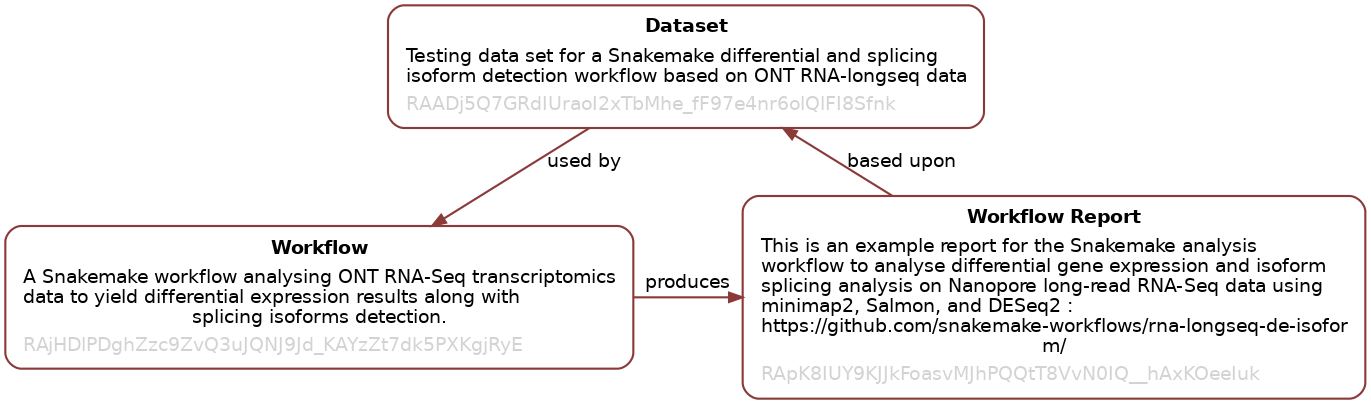
\includegraphics[width=0.8\linewidth]{Snakemake_Metadata.png} \\
        \vspace{0.5em}
        \footnotesize Created with \href{https://github.com/snakemake/snakemake-report-plugin-nanopub/}{the Snakemake reporter plugin for posting workflow metadata}.
        \vspace{1em}
        \begin{callouttip}
            \textbf{Citing Nanopubs} \\
            Remember: nanopubs are unique persistent identifiers, worldwide accessible.
        \end{callouttip}
    }

%%%%%%%%%%%%%%%%%%%%%%%%%%%%%%%%%%%%%%%%%%%%%%%%%%%%%%%%%%%%%%%%%%%%%%%%%%%%%%%%    
    \frame{
        \frametitle{What can you do with Nanopubs? II}
        More \& more Citation Ontologies become available in Scholia:
        \vspace{1em}
        \centering
        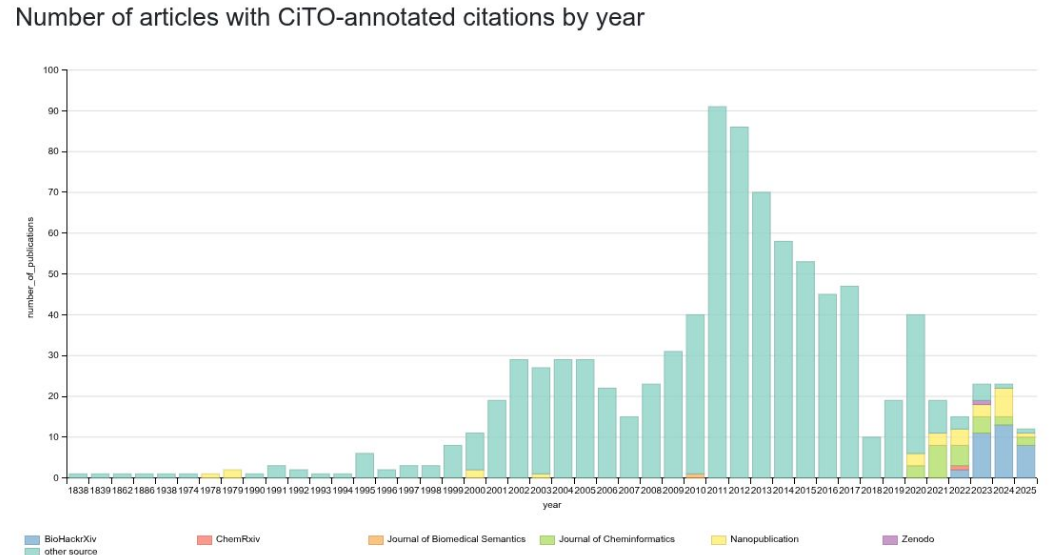
\includegraphics[width=0.8\linewidth]{CiTO_Scholia.png} \\
        \vspace{1em}
        \begin{callouttip}
            \textbf{Nanopub has a Template for your CiTOs} \\
            \href{https://w3id.org/np/RAX_4tWTyjFpO6nz63s14ucuejd64t2mK3IBlkwZ7jjLo}{Declare CiTOs with this template}
        \end{callouttip}
    }

%%%%%%%%%%%%%%%%%%%%%%%%%%%%%%%%%%%%%%%%%%%%%%%%%%%%%%%%%%%%%%%%%%%%%%%%%%%%%%%%    
    \frame{
        \frametitle{And now? Where to go from here?}
        This workshop \textit{merely} gave an overview. There is so much more:
        \begin{itemize}
            \item<+-> \textbf{Community}
            \begin{itemize}
                \item<+-> \href{https://nanopub.net/sessions/}{Nano Sessions} – every last Tuesday of a month; reports from practitioners; ask questions; \\
                \href{https://nanodash.knowledgepixels.com/space?id=https://w3id.org/spaces/nanopub/nanosessions}{register here with a nanopub}
                \item<+-> \href{https://nanodash.knowledgepixels.com/space?id=https://w3id.org/spaces/fenac}{FENAC} – the “Fearless Early Nanopub Adopters Club”; sign-up per nanopub; members get prioritized feature requests and a free one-on-one call with a core developer.
            \end{itemize}
            \item<+-> \textbf{Resources}
            \begin{itemize}
                \item<+-> \href{https://nanopub.net/docs/tutorials/}{Official tutorial selection}
                \item<+-> \href{https://nanopub.net/docs/}{Documentation}
            \end{itemize}
            \item<+-> \textbf{Software with an API for automated publication}
            \begin{itemize}
                \item<+-> \href{https://github.com/Nanopublication/nanopub-java}{Java library}
                \item<+-> \href{https://github.com/Nanopublication/nanopub-py/}{Python library}
            \end{itemize}
            \item<+-> \textbf{Software that uses the API}
            \begin{itemize}
                \item<+-> \href{https://github.com/snakemake/snakemake-report-plugin-nanopub/}{Snakemake reporter plugin for posting workflow metadata}
            \end{itemize}
        \end{itemize}
    }
    


%%%%%%%%%%%%%%%%%%%%%%%%%%%%%%%%%%%%%%%%%%%%%%%%%%%%%%%%%%%%%%%%%%%%%%%%%%%%%%%%
%%%%%%%%%%%%%%%%%%%%%%%%%%%%%%%%%%%%%%%%%%%%%%%%%%%%%%%%%%%%%%%%%%%%%%%%%%%%%%%%%
\section{Snakemake Nanopub Reports}
{   
    \usebackgroundtemplate{
        \vbox to \paperheight{\vfil\hbox to \paperwidth{\hfil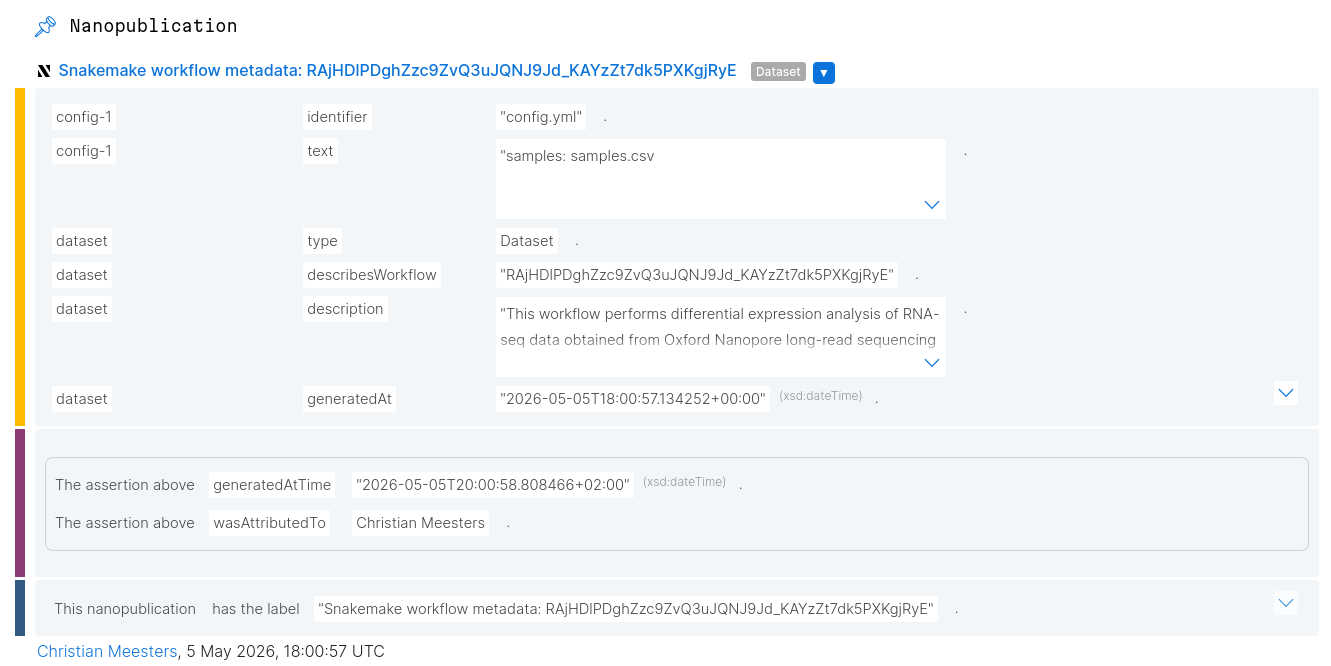
\includegraphics[width=\paperwidth]{reports/nanopub_workflow_report.png}\hfil}\vfil}
    }
    \frame{
        \frametitle{\Snakemake Reports with Nanopubs}
        \begin{mdframed}[tikzsetting={draw=white,fill=white,fill opacity=0.8,
                line width=0pt},backgroundcolor=none,leftmargin=0,
            rightmargin=150,innertopmargin=4pt,roundcorner=10pt]
            \tableofcontents[currentsection,sections={1-4},hideothersubsections]
        \end{mdframed}
        \vfill\vspace{16mm}\hfil \hfill{\tiny Screenshot -- upper section of a registered workflow nanopub}
    }
}

%%%%%%%%%%%%%%%%%%%%%%%%%%%%%%%%%%%%%%%%%%%%%%%%%%%%%%%%%%%%%%%%%%%%%%%%%%%%%%%%
\begin{frame}
    \frametitle{\HandsOn{How to register your Workflow}}
    We created a \lhref{https://w3id.org/np/RAOT7z3RA0XYlHIikne8rfUUYZrtHyrzXBD1HpI_GvcRk}{registration template}: \altverb{RAOT7z3RA0XYlHIikne8rfUUYZrtHyrzXBD1HpI_GvcRk}
    \begin{task}
       Use this template to register a workflow. Possibly \emph{your} workflow? Else the tutorial workflow.\\
       To register a workflow, it needs to be registered with a DOI (or a nanopub itself):
       \begin{itemize}
           \item On Zenodo you can create a DOI via GitHub, e.g. \lhref{https://doi.org/10.5281/zenodo.17087101}{this one}.
           \item Alternatively, \lhref{https://workflowhub.eu/search?q=Snakemake\#workflows}{WorkflowHub} has a few registered workflows -- we will work to extend this.
           \item Or you use \lhref{https://doi.org/10.14279/eceasst.v83.2600}{the DOI for a tutorial workflow}  registered with the HPC teaching alliance for \Snakemake.
       \end{itemize}
    \end{task}
\end{frame}

%%%%%%%%%%%%%%%%%%%%%%%%%%%%%%%%%%%%%%%%%%%%%%%%%%%%%%%%%%%%%%%%%%%%%%%%%%%%%%%%
\begin{frame}
    \frametitle{What if a workflow is registered multiple times?}
    \begin{docs}
        The Nanopublications framework does not prevent this. It is not desirable, but cannot be avoided.
        \begin{itemize}[<+->]
            \item You can retract accidentally created nanopubs (or those with a glitch).
            \item Search before registering \lhref{https://nanodash.knowledgepixels.com/query?id=RApMWbZ0ixGj88tPB4cEamKJQuQTZ5Dxpjh1a5BWteTdE/SnakemakeWorkflowRegistrations}{using this query}. 
        \end{itemize}
    \end{docs}
    \pause
    \begin{hint}
        We will retract unnecessarily created nanopubs, e.g. from the example DOIs.
    \end{hint}
\end{frame}

%%%%%%%%%%%%%%%%%%%%%%%%%%%%%%%%%%%%%%%%%%%%%%%%%%%%%%%%%%%%%%%%%%%%%%%%%%%%%%%%
\begin{frame}[fragile]
    \frametitle{\HandsOn{Using the plugin to create your Nanopub report}}
    First we need to install it into a working \Snakemake environment:
    \begin{lstlisting}[language=Bash, style=Shell]
$ # pip or mamba
$ pip install snakemake-report-plugin-nanopub
    \end{lstlisting}
    Then take your just created nanopub to register your workflow:
    \begin{lstlisting}[language=Bash, style=Shell]
$ snakemake ... --reporter nanopub \
> --report-nanopub-workflow-id <nanopub workflow id>
    \end{lstlisting}
    \begin{warning}
        This may trigger a workflow to run!
    \end{warning}
\end{frame}

%%%%%%%%%%%%%%%%%%%%%%%%%%%%%%%%%%%%%%%%%%%%%%%%%%%%%%%%%%%%%%%%%%%%%%%%%%%%%%%%
\begin{frame}[fragile]
    \frametitle{\HandsOn{Browsing the report}}
    Browse your own nanopub report or \lhref{https://w3id.org/np/RAK9xz_ccnu0Xhs4vX2KtqCxX44mmSt6nq-ePLeewMrFE}{this one}
    \begin{hint}
        Basically you can use this to simplify a materials \& methods section of a paper like this:\\
        
        
    \end{hint}
\end{frame}

%%%%%%%%%%%%%%%%%%%%%%%%%%%%%%%%%%%%%%%%%%%%%%%%%%%%%%%%%%%%%%%%%%%%%%%%%%%%%%%%
\begin{frame}
    \frametitle{An example knowledge graph}
    To visualize the result we can use the plugin to create a graph like this:
    \begin{centering}
    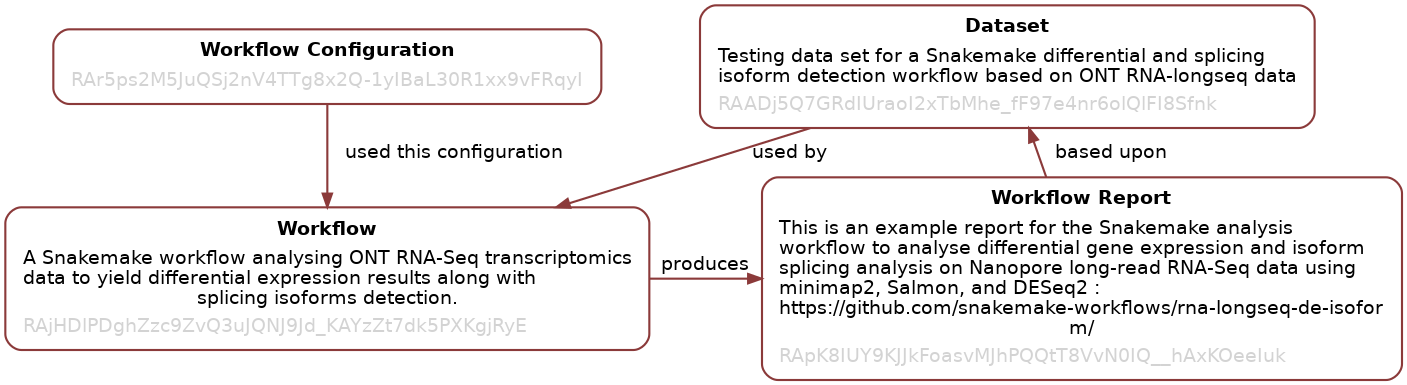
\includegraphics[width=0.9\textwidth]{reports/example_knowledgegraph.png}
    \end{centering}
    \begin{hint}
        It will contain the descriptions the workflow designer (you?) entered into the workflow, the dataset, etc..
    \end{hint}
\end{frame}

%%%%%%%%%%%%%%%%%%%%%%%%%%%%%%%%%%%%%%%%%%%%%%%%%%%%%%%%%%%%%%%%%%%%%%%%%%%%%%%%
\begin{frame}[fragile]
    \frametitle{Creating this knowledge graph}
    The nanopub reporter plugin for \Snakemake has a script on board:
    \begin{lstlisting}[language=Bash, style=Shell]
$ plot-nanopub-knowledge-graph \
> --dataset-nanopub-id <dataset_id> \
> --workflow-nanopub-id <id of registered workflow> \
> --workflow-configuration-id <id of registered conf> \
> --report-nanopub-id <id of registered report> \ 
> -o example_knowledgegraph.png
    \end{lstlisting}
    \begin{hint}
        \begin{itemize}
            \item file type determined by suffix (\altverb{png}, \altverb{pdf}, \altverb{svg})
            \item all flags are mandatory
        \end{itemize}
    \end{hint}
\end{frame}


%%%%%%%%%%%%%%%%%%%%%%%%%%%%%%%%%%%%%%%%%%%%%%%%%%%%%%%%%%%%%%%%%%%%%%%%%%%%%%%% 
\begin{frame}<handout:0> 
	\frametitle{The End}
	\begin{center}
		\begin{figure}
			\centering
			
			
\includegraphics[width=0.7\textwidth]{logos/the_end.jpg}
		\end{figure}
		Thank you for your attention!
	\end{center}
\end{frame}

\begin{frame}<beamer:0> 
	\frametitle{End of the Talk}

\end{frame}

\end{document}

